
\section{Identificación de propuestas regioquímicas y funcionalización secuencial de C\textsubscript{60} con glicina}

Para estudiar la funcionalización de la jaula de C\textsubscript{60} con glicina, se realizaron cálculos de optimización geométrica y análisis de frecuencias vibracionales mediante la teoría del funcional de la densidad (DFT), empleando el funcional híbrido B3LYP y el conjunto de bases 6-311G(d,p). La ausencia de frecuencias imaginarias permitió confirmar que las estructuras optimizadas corresponden a mínimos locales en la superficie de energía potencial, dentro del nivel de teoría utilizado. Adicionalmente, se calcularon las funciones de Fukui con el propósito de identificar regiones de la jaula susceptibles a la adición de nuevas moléculas de glicina.

Debido a la simetría icosaédrica del C\textsubscript{60} prístino, sus 60 átomos de carbono son equivalentes por simetría. Por esta razón, para estudiar la primera adición se mantuvo el carbono C59 como sitio de unión del grupo derivado de la glicina y se modificó la posición del átomo de hidrógeno incorporado a la jaula. De esta manera se obtuvieron seis propuestas regioquímicas, correspondientes a diferentes posiciones de adición sobre la superficie del fullereno.

En la Figura~\ref{fig:isomeros-gly1-2} se muestran las seis estructuras propuestas. Los isómeros a y b corresponden a las posiciones C59--C43 y C59--C58, respectivamente, mientras que los isómeros c y d representan adiciones sobre los pares C59--C11 y C59--C10. Estos últimos permiten comparar configuraciones vicinales asociadas con enlaces de tipo [6,6] y [5,6], respectivamente. Por su parte, los isómeros e y f corresponden a las posiciones C59--C50 y C59--C51, consideradas para ampliar la comparación a otras regiones de la jaula.

\begin{figure}[H]
      \centering
      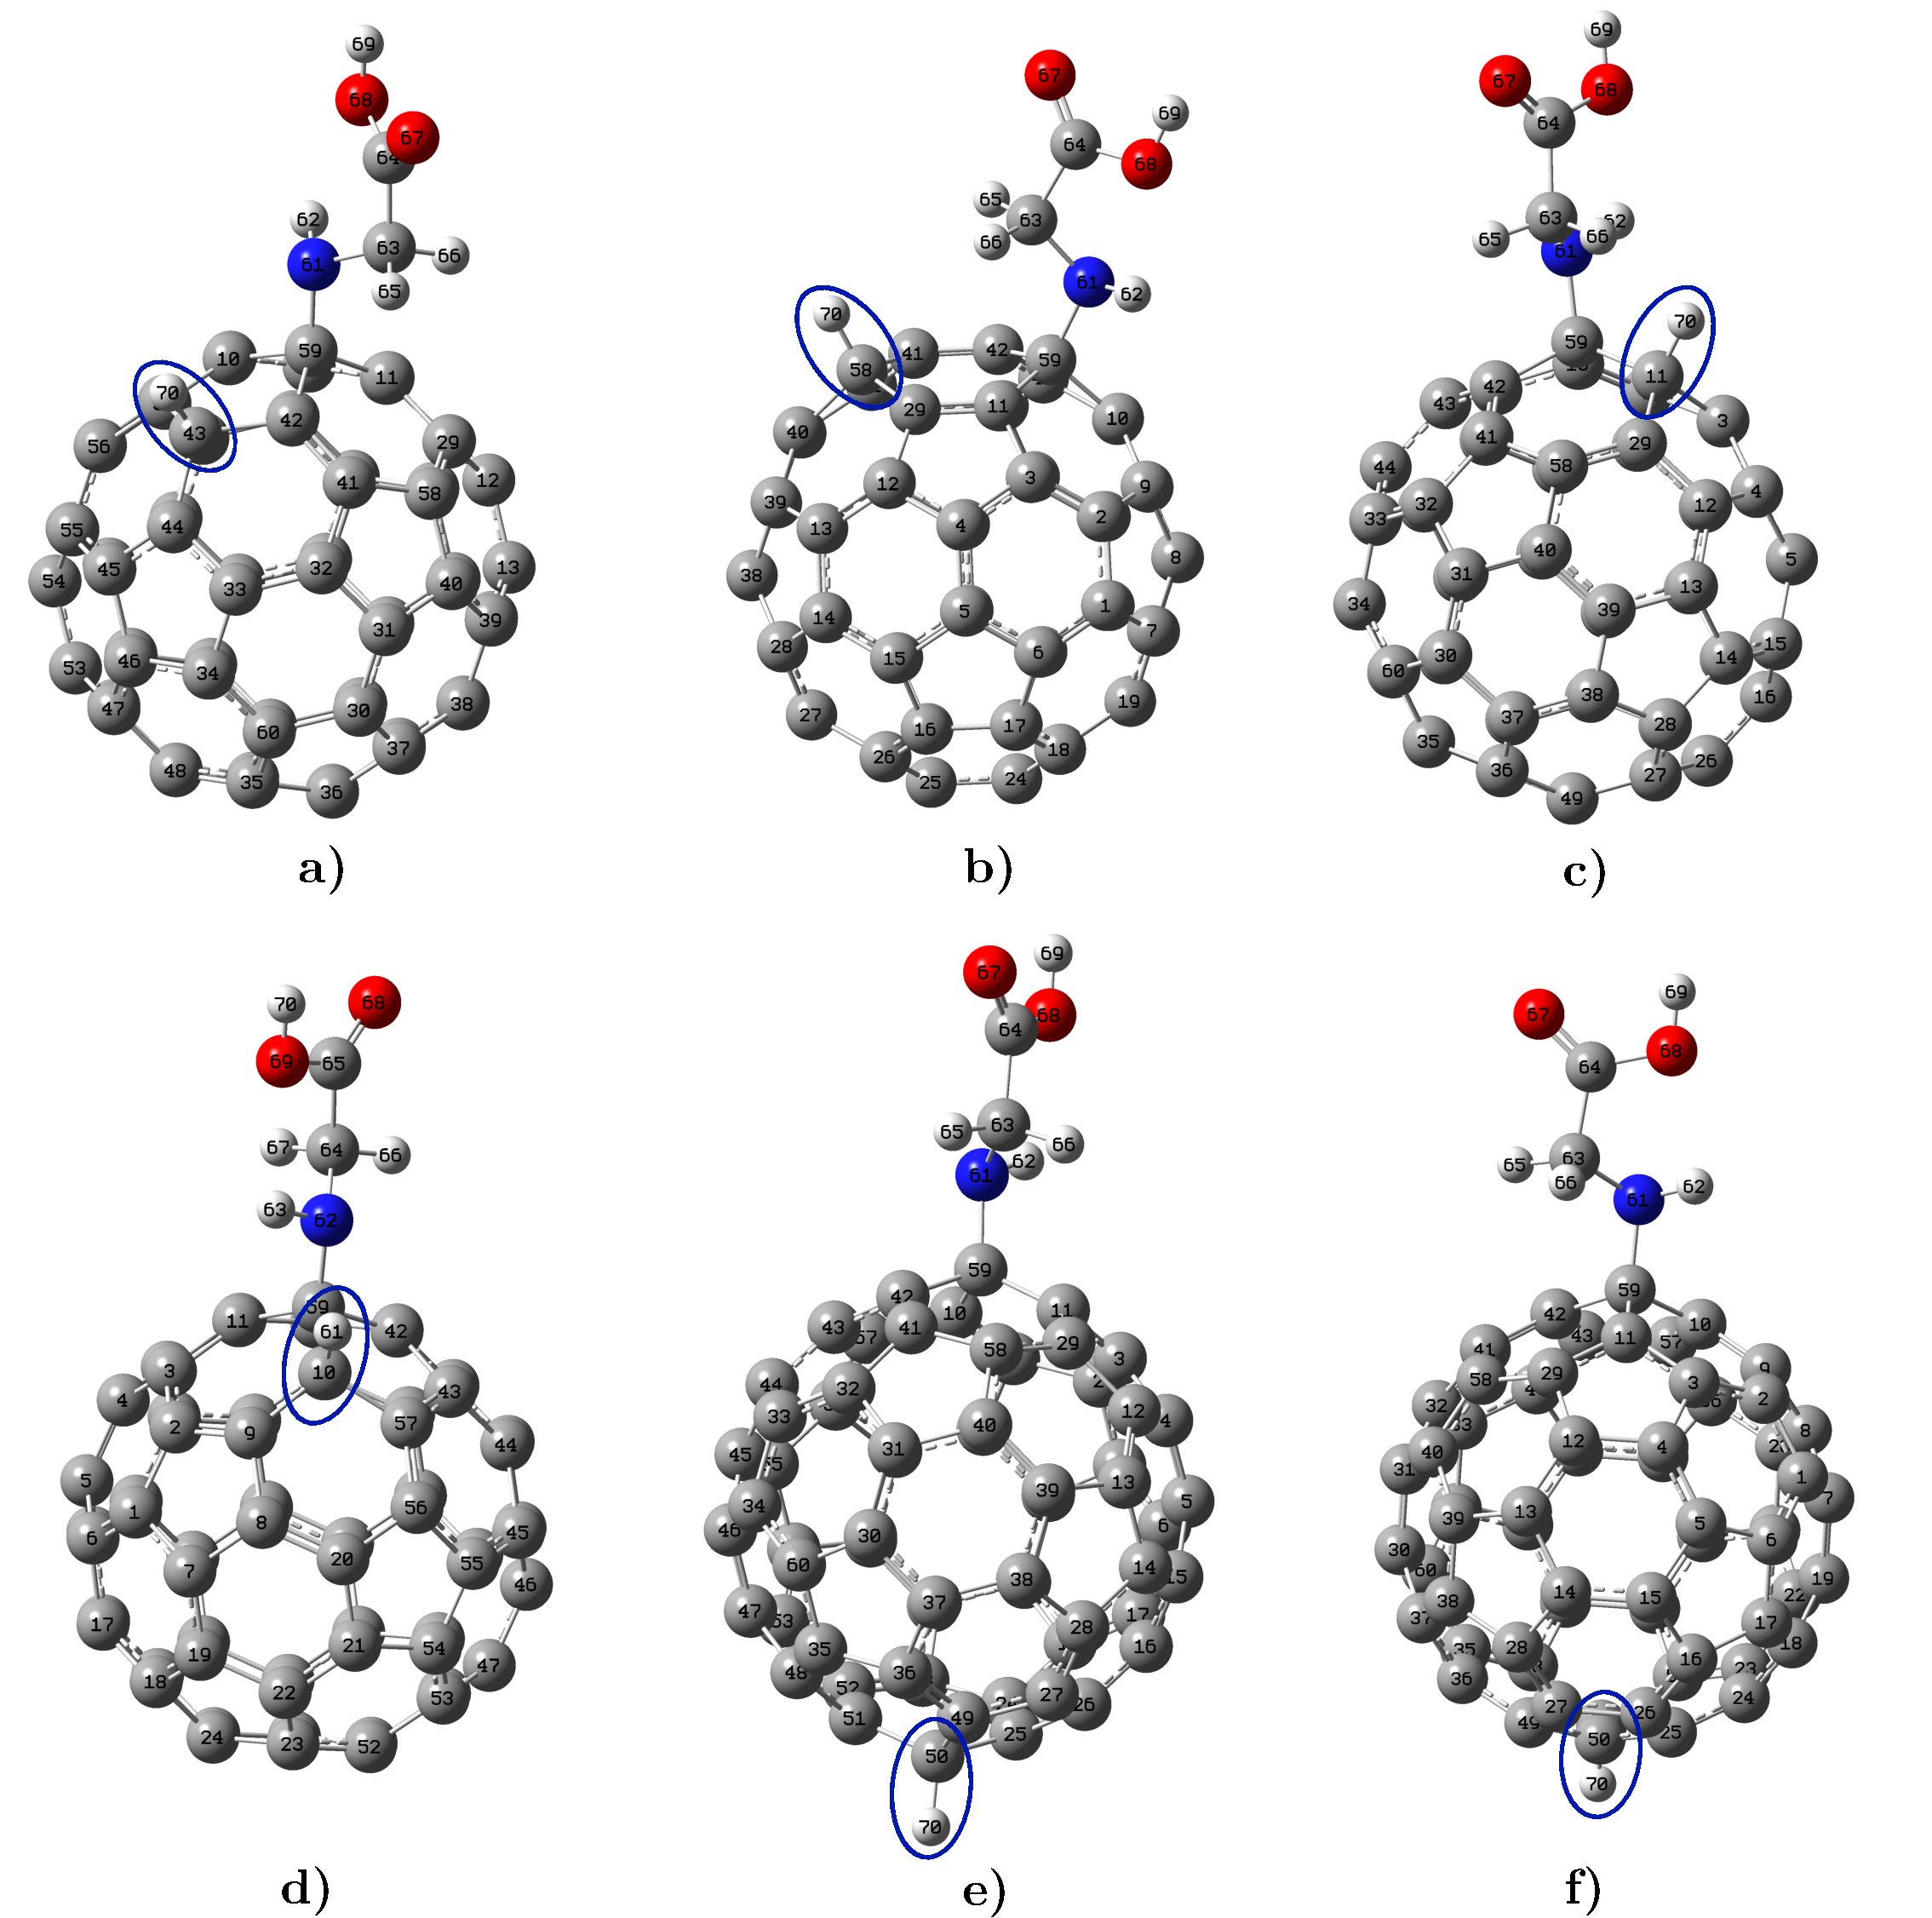
\includegraphics[width=1.0\textwidth]{imagenes/Resu/resu-1-opt.pdf}
      \caption{Isómeros propuestos para la primera adición de glicina al C\textsubscript{60}. La glicina se une al carbono C59; los círculos azules señalan el segundo carbono del enlace evaluado: (a) C43, (b) C58, (c) C11, (d) C10, (e) C50 y (f) C51.}
      \label{fig:isomeros-gly1-2}
        \end{figure}
        
Las energías relativas obtenidas para estas estructuras se presentan en la Tabla~\ref{tab:isomeros-gly1}. El isómero C\textsubscript{60}(Gly)-c, correspondiente a los carbonos C59 y C11, presentó la menor energía y se estableció como estructura de referencia con un valor de 0.000 kcal mol$^{-1}$. Los demás isómeros mostraron diferencias energéticas comprendidas entre 0.010 y 0.074 kcal mol$^{-1}$, siendo C\textsubscript{60}(Gly)-e el de mayor energía relativa.
        
  \begin{itemize}
    \item \textbf{Isómero C\textsubscript{60}(Gly)-a (C59, C43):} El átomo de hidrógeno se localiza en una posición frontal sobre la cara del pentágono con respecto al grupo glicina.
    \item \textbf{Isómero C\textsubscript{60}(Gly)-b (C59, C58):} Representa una disposición de adición en posición \textit{para} en la red hexagonal contigua con respecto a la glicina.
    \item \textbf{Isómero C\textsubscript{60}(Gly)-c (C59, C11):} Corresponde a una adición vicinal (1,2) en posición \textit{orto} a través de un enlace de tipo [6,6] (fusión hexágono-hexágono).
    \item \textbf{Isómero C\textsubscript{60}(Gly)-d (C59, C10):} Constituye una adición vicinal (1,2) a través de un enlace de tipo [5,6] (fusión pentágono-hexágono) entre los carbonos C59 y C10.
    \item \textbf{Isómero C\textsubscript{60}(Gly)-e (C59, C50):} Propuesta diseñada en una región opuesta (antípoda) de la jaula con el fin de evaluar y descartar si las interacciones a larga distancia o la polarización de la red generan una mayor estabilidad termodinámica.
    \item \textbf{Isómero C\textsubscript{60}(Gly)-f (C59, C51):} Corresponde a la funcionalización en un carbono adyacente a la posición opuesta evaluada en el inciso (e).
\end{itemize}

\begin{table}[H]
    \centering
    \caption{Energías de formación de los isómeros del complejo C\textsubscript{60}(Gly).Energías relativas de los seis isómeros propuestos para la primera adición de glicina a C\textsubscript{60}(Gly) }
    \label{tab:isomeros-gly1}
    \renewcommand{\arraystretch}{1.15}
    \begin{tabular}{lcc}
        \toprule
        \textbf{Isómero} & \textbf{Carbonos de enlace} & \textbf{Energía relativa (kcal mol$^{-1}$)} \\
        \midrule
      C\textsubscript{60}(Gly)-a & C59, C43 & 0.059 \\
      C\textsubscript{60}(Gly)-b & C59, C58 & 0.010 \\
       \textbf{  C\textsubscript{60}(Gly)-c} &\textbf{ C59, C11} & \textbf{0.000} \\
         C\textsubscript{60}(Gly)-d & C59, C10 & 0.027 \\
        C\textsubscript{60}(Gly)-e & C59, C50 & 0.074 \\
         C\textsubscript{60}(Gly)-f & C59, C51 & 0.045 \\
        \bottomrule
    \end{tabular}
\end{table}      
        
  Como puede observarse, las diferencias energéticas entre los seis isómeros son pequeñas, lo que indica que presentan energías muy similares al nivel de teoría empleado. Aunque el isómero C\textsubscript{60}(Gly)-c corresponde a la estructura de menor energía entre las evaluadas, no se observa una preferencia energética marcada respecto a las demás configuraciones. Asimismo, estas diferencias no permiten establecer cuál de los isómeros se formaría preferentemente durante una reacción, ya que para ello sería necesario conocer las barreras de activación de las distintas rutas de adición.

Considerando los resultados obtenidos, se seleccionó el isómero C\textsubscript{60}(Gly)-c como estructura de partida para continuar con la funcionalización de la jaula. A partir de esta geometría optimizada se calcularon las funciones de Fukui para ataque nucleofílico ($f^{+}$), con el propósito de identificar regiones susceptibles a recibir densidad electrónica. La distribución espacial de estas funciones se visualizó utilizando un isovalor de 0.003 a.u., lo que permitió proponer diferentes posiciones para la incorporación de las siguientes moléculas de glicina.

Para la segunda adición se consideraron cuatro sitios candidatos sobre el sistema C\textsubscript{60}(Gly)-c. Las estructuras optimizadas correspondientes se muestran en la Figura~\ref{fig:secuencia-gly}. Los pares de carbonos evaluados fueron C31--C30, C07--C19, C28--C27 y C54--C53, correspondientes a los candidatos a, b, c y d, respectivamente. Estas posiciones se seleccionaron a partir del análisis de reactividad local y posteriormente se compararon sus energías relativas.   

           
    \begin{figure}[H]
      \centering
      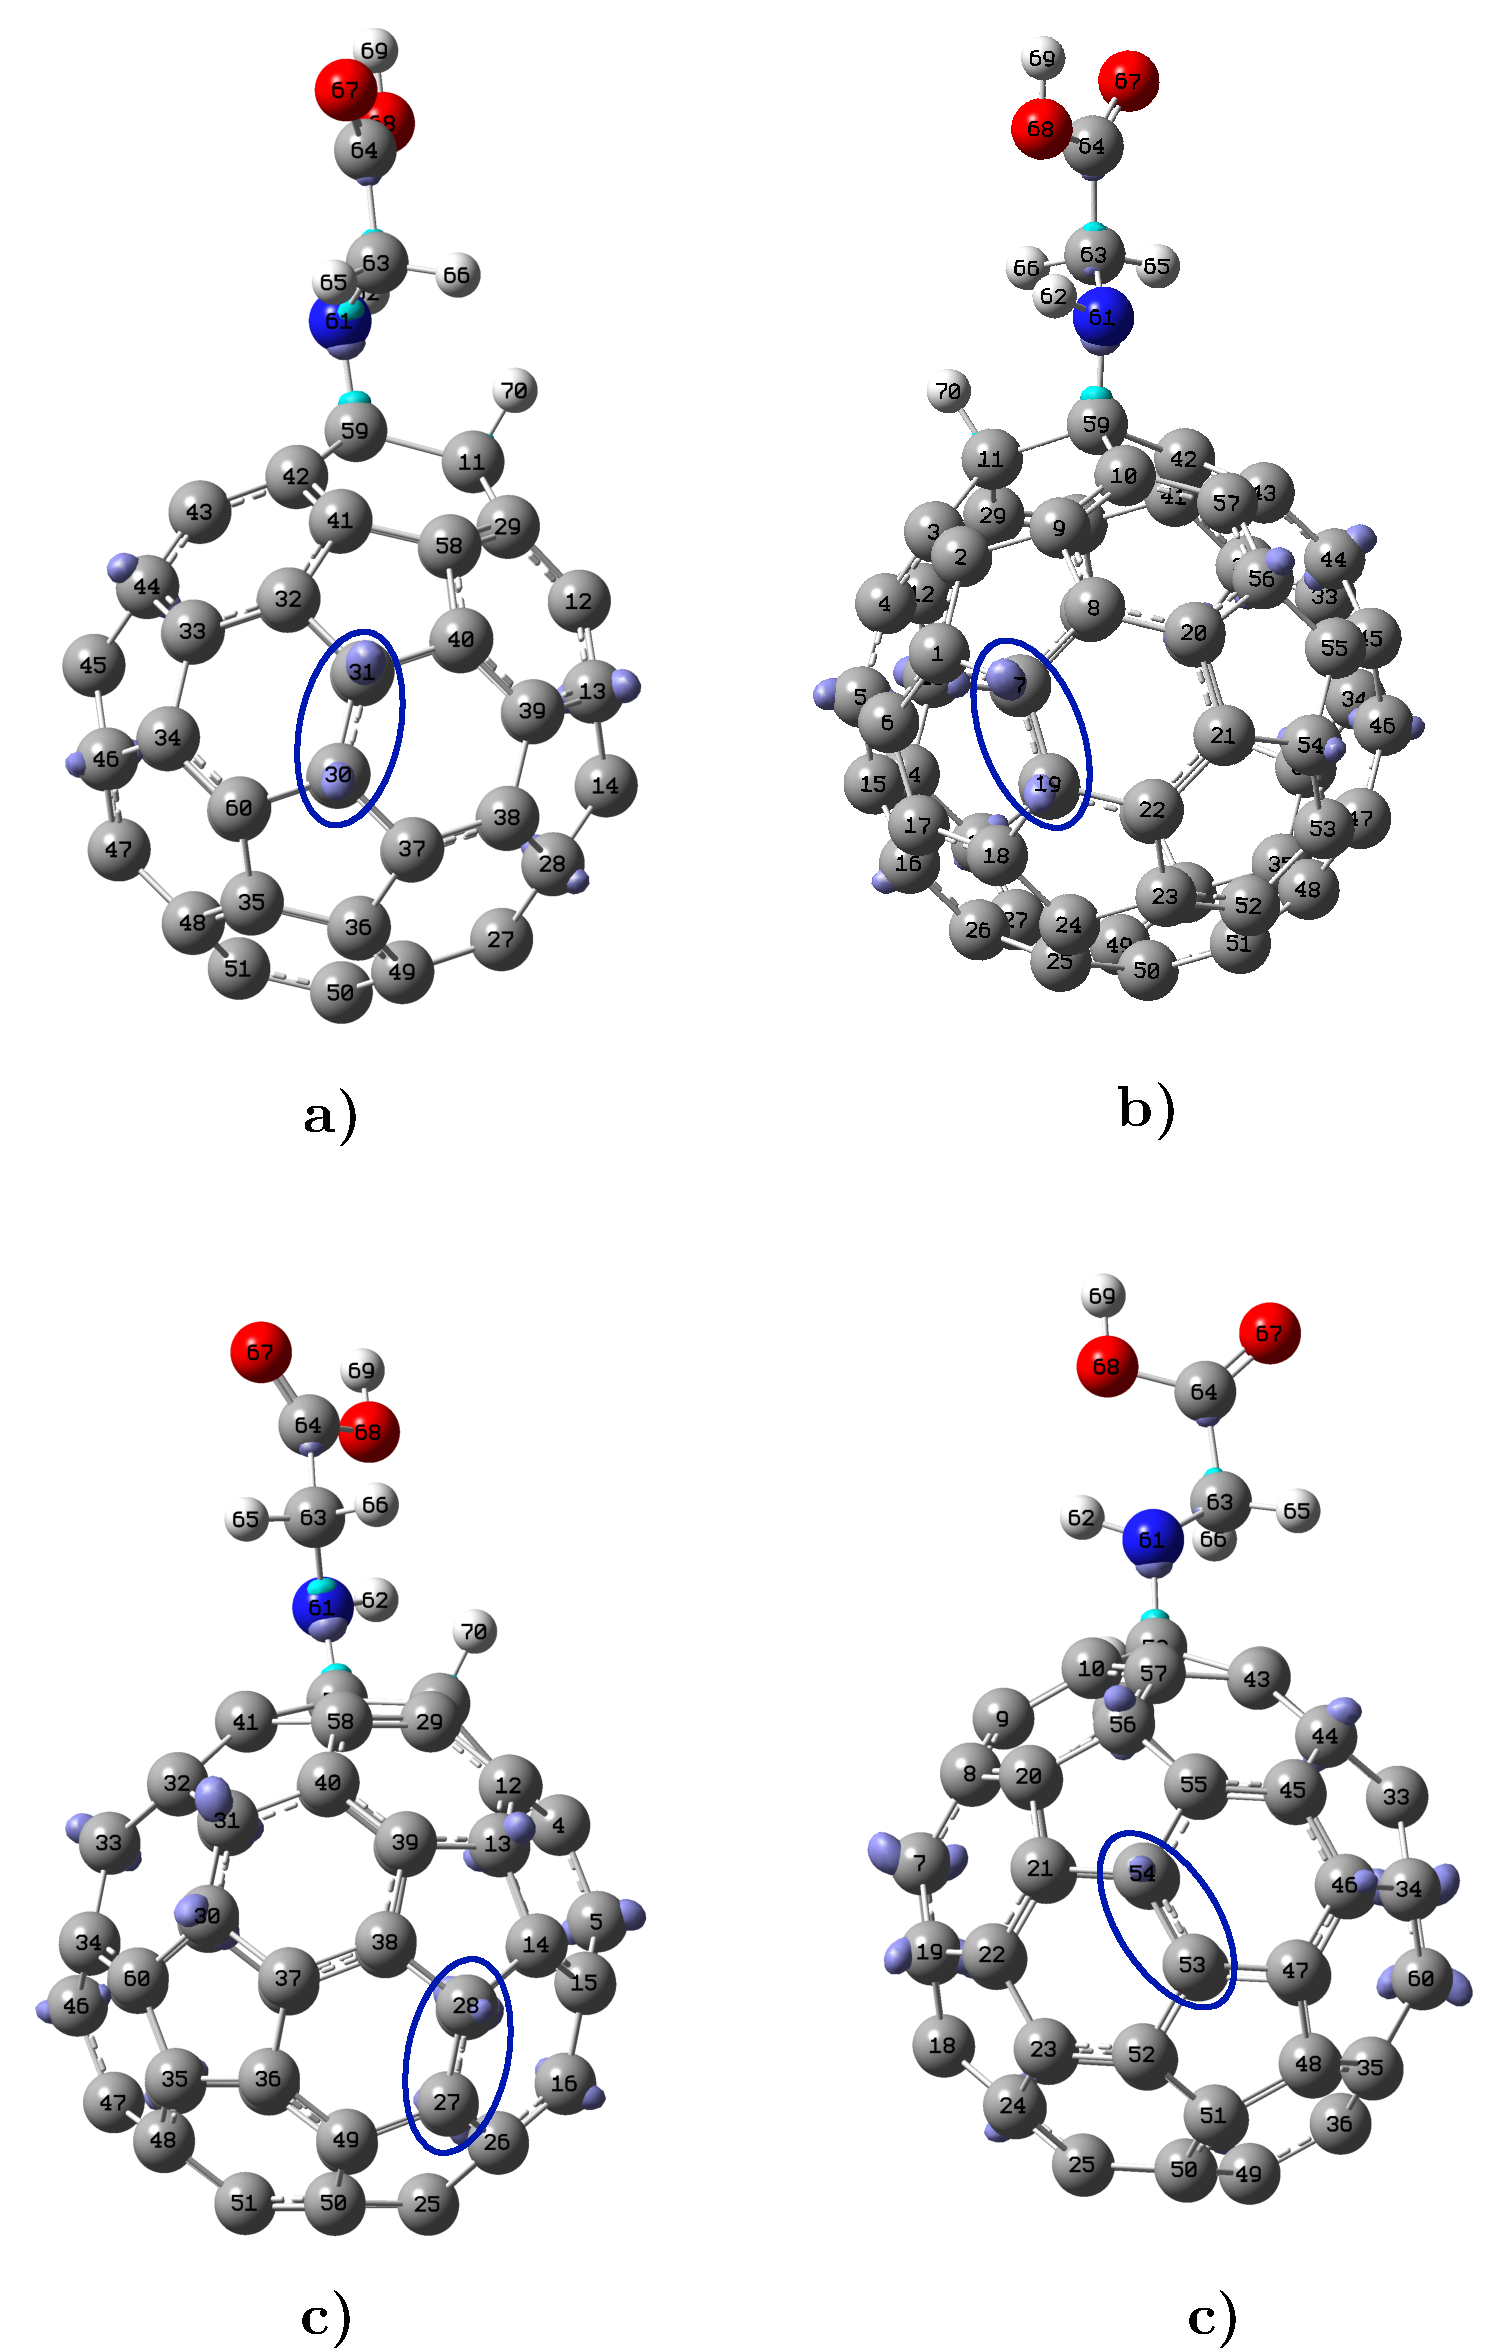
\includegraphics[width=0.7\textwidth]{imagenes/Resu/fukui-gly-resul-1.pdf}
      \caption{Estructuras seleccionadas durante la funcionalización secuencial de la jaula de C\textsubscript{60} con glicina. Los paneles muestran los sistemas con uno, dos, tres y cuatro grupos de glicina, respectivamente.}
      \label{fig:secuencia-gly}
        \end{figure}    
             
Una vez obtenidas las estructuras correspondientes a la segunda adición, se tomó la configuración de menor energía entre las evaluadas para continuar con la incorporación de una tercera molécula de glicina. Para ello se analizaron nuevamente las funciones de Fukui del sistema C\textsubscript{60}(Gly)\textsubscript{2}, identificando cuatro posibles posiciones de adición. Las alternativas consideradas se muestran en la Figura~\ref{fig:isomeros-gly3}, donde los círculos azules indican los pares de carbonos evaluados.

 \begin{figure}[H]
      \centering
      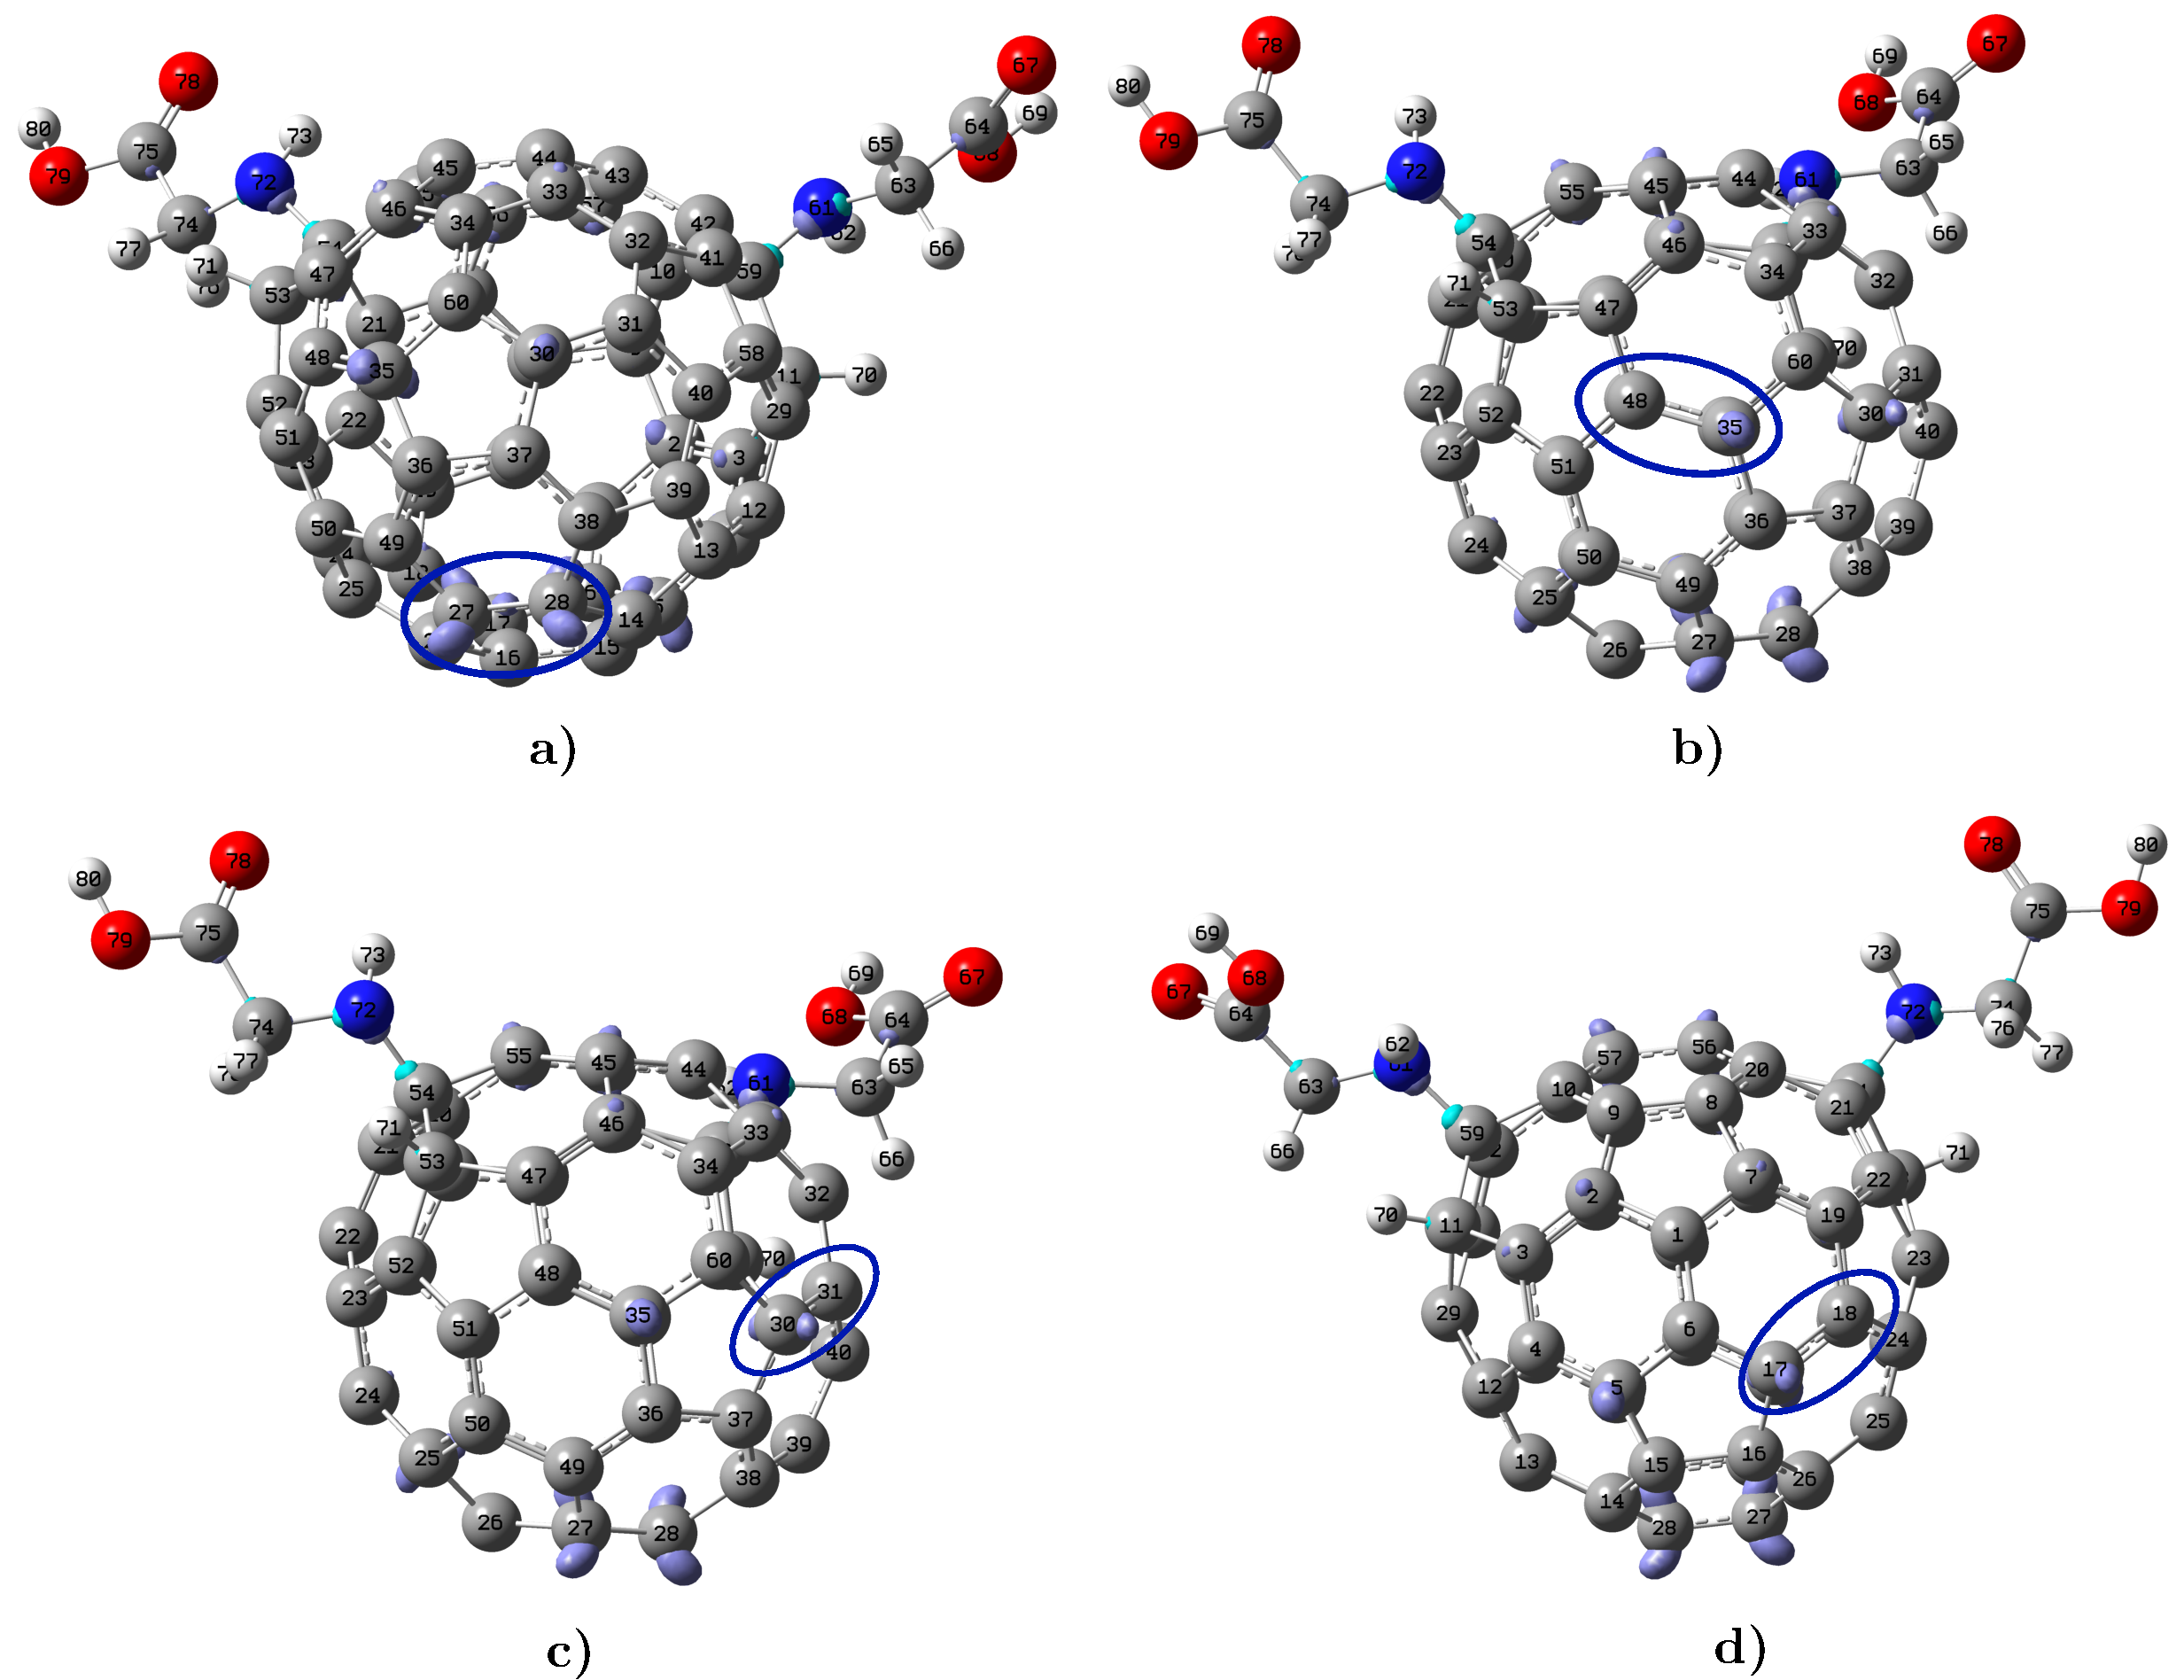
\includegraphics[width=1.0\textwidth]{imagenes/Resu/resu-2-fukui.pdf}
      \caption{Alternativas estructurales consideradas para continuar la funcionalización de C\textsubscript{60} con un tercer grupo de glicina. Los círculos azules indican los pares de carbonos evaluados como sitios de adición.}
      \label{fig:isomeros-gly3}
        \end{figure} 
        
 De manera similar, para la incorporación de una cuarta molécula de glicina se analizaron nuevas posiciones sobre el sistema C\textsubscript{60}(Gly)\textsubscript{3}. Las cuatro alternativas propuestas se muestran en la Figura~\ref{fig:isomeros-gly2}. En esta etapa se consideraron los pares de carbonos C52--C23, C29--C58, C49--C36 y C14--C15, correspondientes a los candidatos a, b, c y d, respectivamente.
\begin{figure}[H]
      \centering
      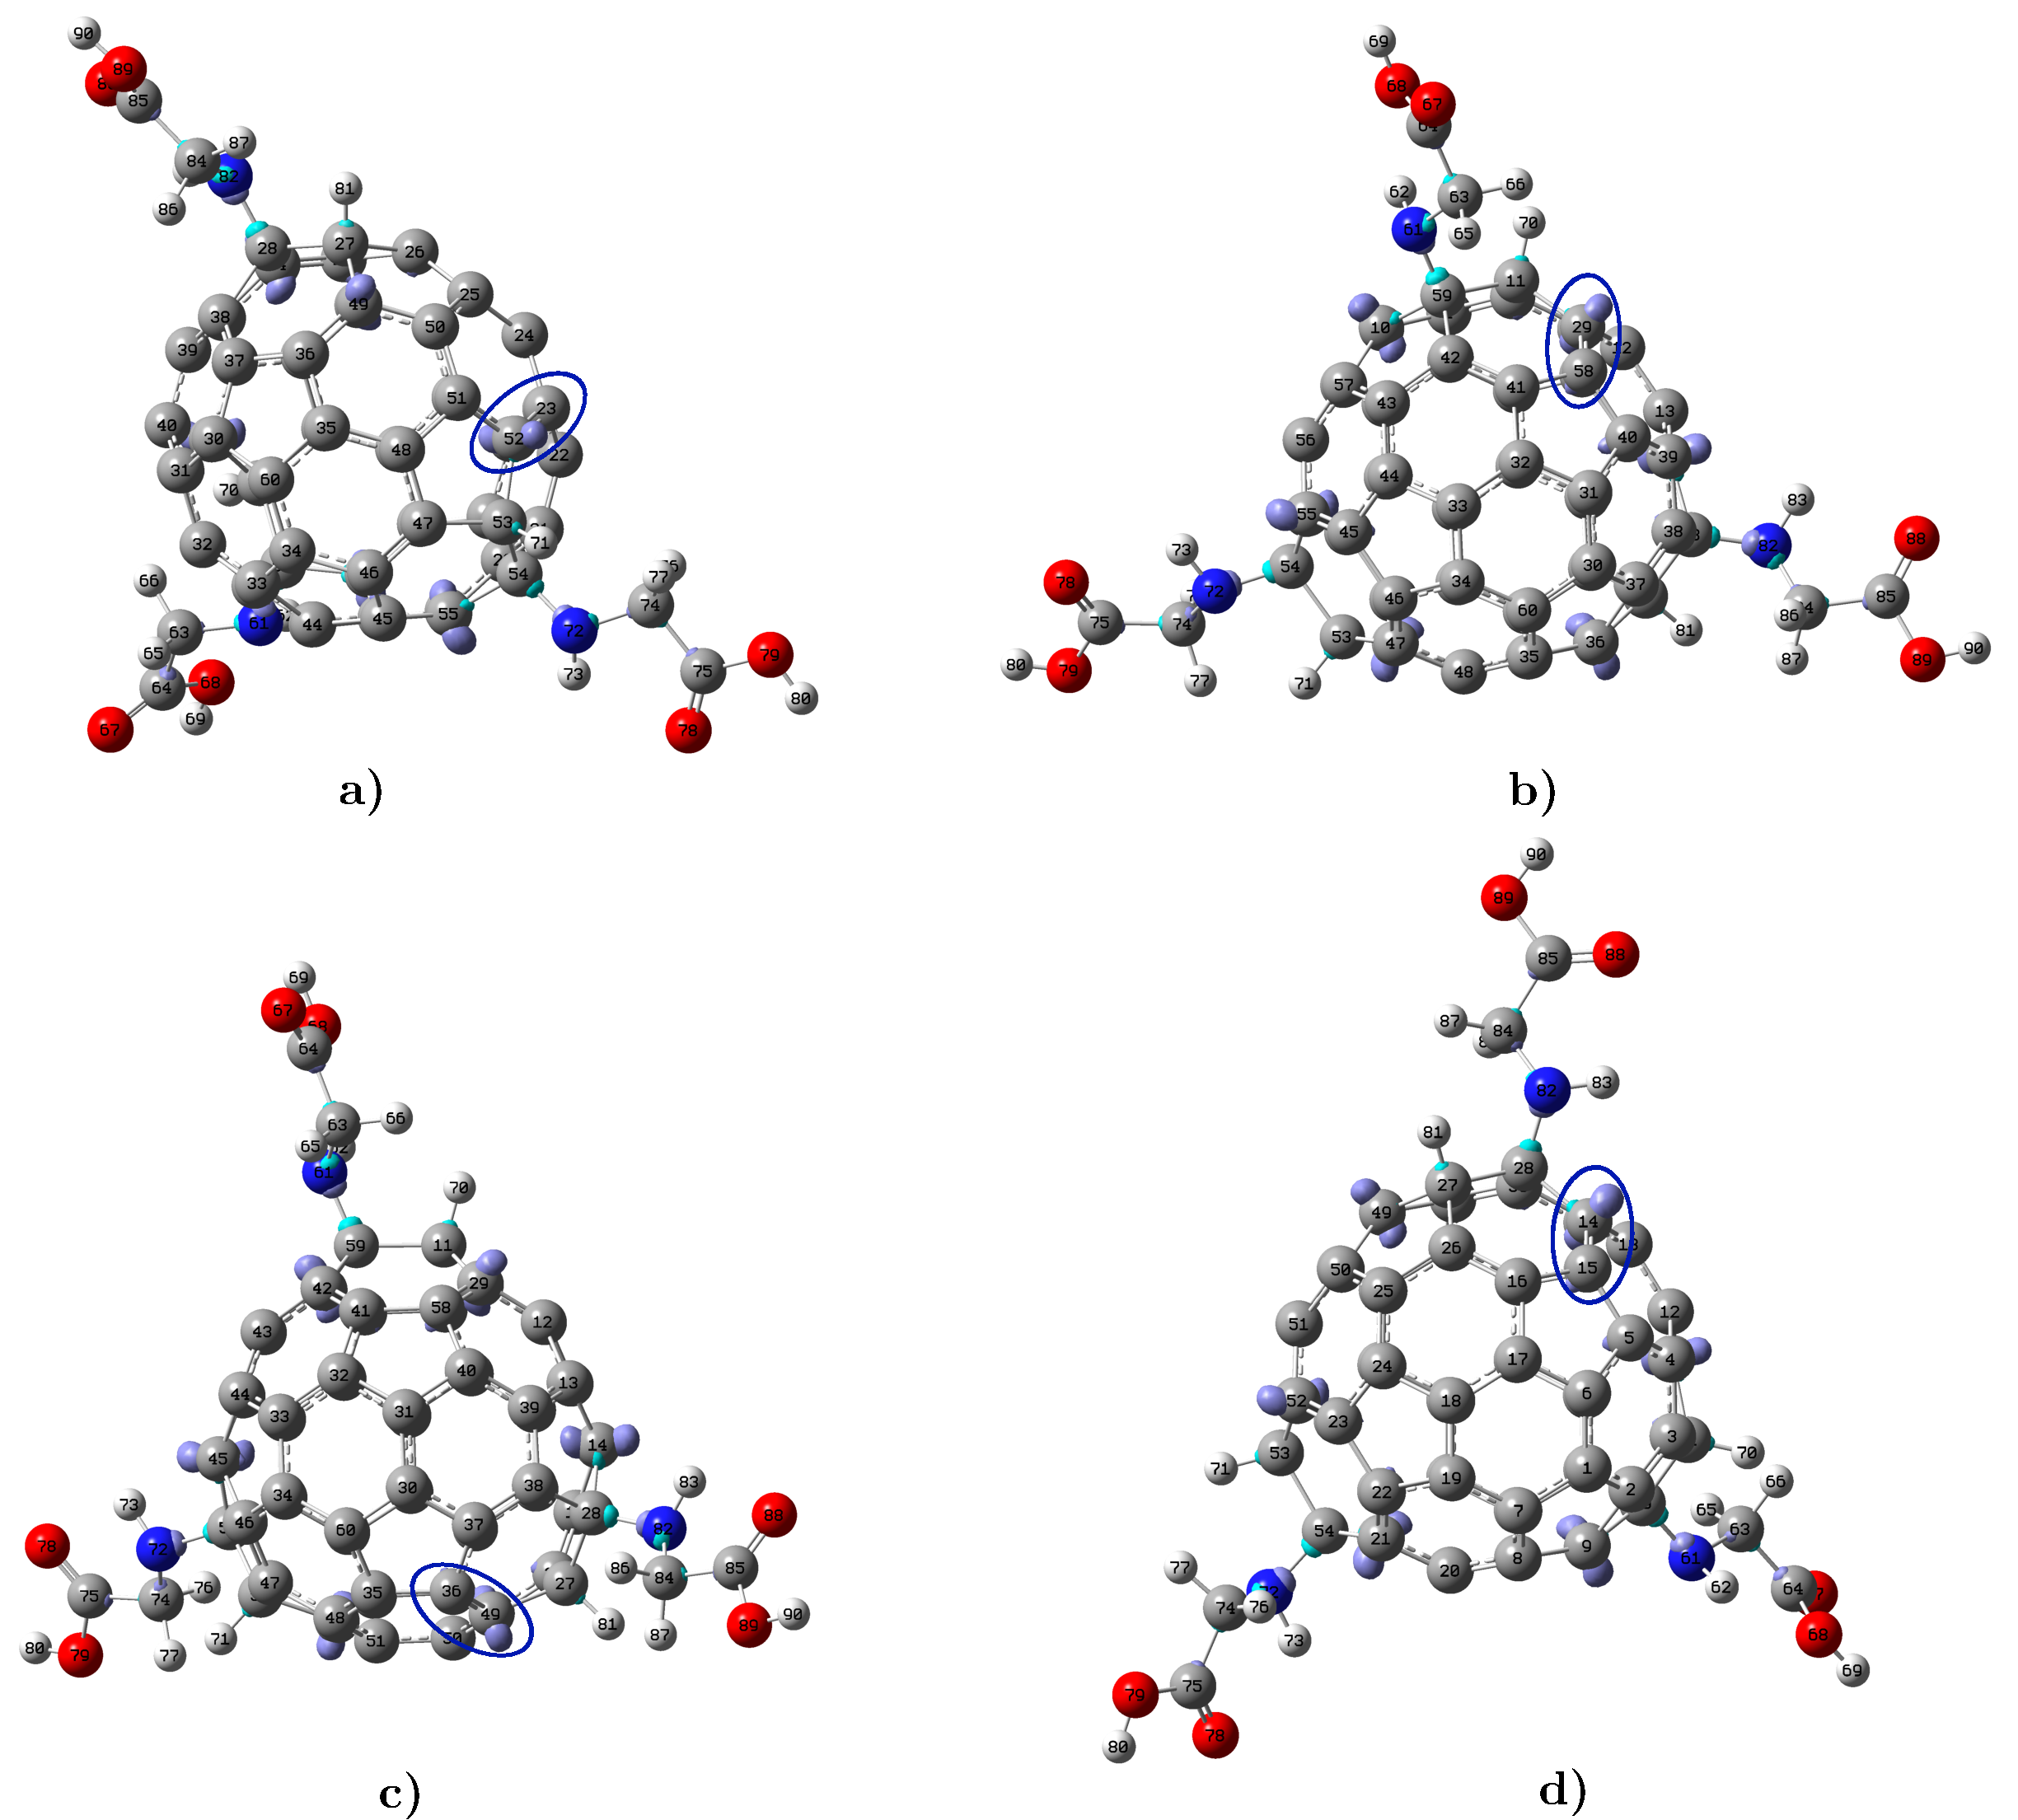
\includegraphics[width=1.0\textwidth]{imagenes/Resu/resu-3-fukui.pdf}
      \caption{Alternativas estructurales consideradas para la cuarta adición de glicina al sistema C\textsubscript{60}(Gly)\textsubscript{3}. Los círculos azules señalan los pares de carbonos analizados para formar el complejo C\textsubscript{60}(Gly)\textsubscript{4}.}
      \label{fig:isomeros-gly4}
        \end{figure}            

 Las energías relativas obtenidas para la segunda, tercera y cuarta adición se presentan en la Tabla~\ref{tab:adicion-secuencial-gly}. Para cada etapa se tomó como referencia la estructura de menor energía entre las alternativas evaluadas, lo que permitió comparar las diferentes posiciones propuestas dentro de cada sistema.
 
 \begin{table}[H]
    \centering
    \caption{Sitios candidatos para la adición secuencial de glicina en C\textsubscript{60}, propuestos a partir de los índices de reactividad de Fukui. La selección identifica el sitio empleado para continuar la funcionalización.}
    \label{tab:adicion-secuencial-gly}
    \renewcommand{\arraystretch}{1.15}
    \begin{threeparttable}
        \begin{tabular}{clcc}
            \toprule
            \textbf{Sistema} & \textbf{Candidato} & \textbf{Carbonos de adición} & \textbf{Energía relativa (kcal mol$^{-1}$)} \\
            \midrule
            \multirow{4}{*}{C\textsubscript{60}(Gly)\textsubscript{2}}
              & a) & C31, C30 & 0.696 \\
              & b) & C07, C19 & 0.789 \\
              & c) & C28, C27 & 0.850 \\
              & \textbf{d)} & \textbf{C54, C53} & \textbf{0.000} \\
            \addlinespace
            \multirow{4}{*}{C\textsubscript{60}(Gly)\textsubscript{3}}
              & \textbf{a)} & \textbf{C28, C27} & \textbf{0.000} \\
              & b) & C35, C48 & 3.935 \\
              & c) & C30, C31 & 1.142 \\
              & d) & C17, C18 & 1.208 \\
            \addlinespace
            \multirow{4}{*}{C\textsubscript{60}(Gly)\textsubscript{4}}
              & a) & C52, C23 & 0.676 \\
              & \textbf{b)} & \textbf{C29, C58} & \textbf{0.000} \\
              & c) & C49, C36 & 0.640 \\
              & d) & C14, C15 & 2.180 \\
            \bottomrule
        \end{tabular}
        \begin{tablenotes}[flushleft]
            \footnotesize \item Los valores en negritas corresponden a las posiciones seleccionadas en los cálculos originales para la siguiente etapa de funcionalización.
        \end{tablenotes}
    \end{threeparttable}
\end{table}
       
 Para la segunda adición, el candidato d, correspondiente a los carbonos C54 y C53, presentó la menor energía, con un valor de referencia de 0.000 kcal mol$^{-1}$. Los candidatos a, b y c mostraron energías relativas de 0.696, 0.789 y 0.850 kcal mol$^{-1}$, respectivamente. Las diferencias entre las cuatro estructuras son inferiores a 1 kcal mol$^{-1}$, lo que indica que presentan energías relativamente próximas. Estas variaciones pueden estar relacionadas con las diferencias geométricas y electrónicas que se producen al incorporar una segunda molécula de glicina en distintas posiciones de la jaula. A partir de esta comparación se seleccionó la estructura correspondiente a los carbonos C54 y C53 para continuar con la funcionalización.

En la tercera adición se encontró una mayor separación energética entre las estructuras evaluadas. El candidato a, correspondiente a los carbonos C28 y C27, presentó la menor energía y se estableció como referencia con un valor de 0.000 kcal mol$^{-1}$. Los candidatos c y d mostraron diferencias energéticas de 1.142 y 1.208 kcal mol$^{-1}$, respectivamente, mientras que el candidato b, correspondiente a los carbonos C35 y C48, presentó la mayor diferencia, con 3.935 kcal mol$^{-1}$.

A diferencia de la segunda adición, en esta etapa se observa una mayor variación entre las energías relativas de las estructuras propuestas. Esto indica que la posición de incorporación de la tercera molécula de glicina influye sobre la energía de las configuraciones estudiadas. Las diferencias encontradas pueden estar relacionadas con cambios en la geometría de la jaula, la distribución electrónica y las interacciones entre los grupos previamente incorporados. Sin embargo, a partir de las energías relativas no es posible determinar cuál de estos factores presenta la mayor contribución. Debido a que el candidato a mostró la menor energía entre las alternativas consideradas, se seleccionó la estructura correspondiente a los carbonos C28 y C27 para continuar con la cuarta adición.

Finalmente, para la formación del sistema C\textsubscript{60}(Gly)\textsubscript{4}, el candidato b, correspondiente a los carbonos C29 y C58, presentó la menor energía, con un valor de referencia de 0.000 kcal mol$^{-1}$. Los candidatos c y a mostraron diferencias energéticas de 0.640 y 0.676 kcal mol$^{-1}$, respectivamente, mientras que el candidato d, correspondiente a los carbonos C14 y C15, presentó la mayor diferencia, con 2.180 kcal mol$^{-1}$.

En esta última etapa se encontró que tres de las cuatro estructuras presentan diferencias energéticas inferiores a 0.7 kcal mol$^{-1}$, mientras que el candidato d se encuentra a una energía mayor. Esto indica que distintas posiciones de incorporación de la cuarta molécula de glicina conducen a estructuras con energías relativamente próximas. Las diferencias observadas pueden estar relacionadas con la disposición espacial de los grupos funcionales y los cambios estructurales producidos durante la adición. No obstante, sería necesario realizar un análisis adicional de las geometrías optimizadas y de las interacciones intramoleculares para determinar el origen de estas diferencias. Con base en los resultados obtenidos, se seleccionó el candidato b, correspondiente a los carbonos C29 y C58, como estructura final del sistema C\textsubscript{60}(Gly)\textsubscript{4}.

En conjunto, los resultados muestran que las diferencias energéticas entre las estructuras propuestas varían conforme aumenta el número de moléculas de glicina incorporadas a la jaula de C\textsubscript{60}. Para la primera adición, las seis configuraciones presentaron diferencias inferiores a 0.1 kcal mol$^{-1}$, mientras que para la segunda adición la diferencia máxima fue de 0.850 kcal mol$^{-1}$. En la tercera y cuarta adición se encontraron separaciones energéticas mayores, de hasta 3.935 y 2.180 kcal mol$^{-1}$, respectivamente. Estos resultados muestran que la posición de incorporación de los grupos de glicina influye sobre la energía de las estructuras obtenidas, aunque no permiten establecer una relación directa entre el número de grupos incorporados y el impedimento estérico del sistema.

De esta manera, el análisis de las funciones de Fukui permitió proponer posibles sitios de adición a partir de la susceptibilidad electrónica local, mientras que la comparación de energías relativas proporcionó un criterio para seleccionar las estructuras de menor energía entre las alternativas evaluadas. Con base en ambos análisis se estableció una secuencia de funcionalización que parte del isómero C\textsubscript{60}(Gly)-c y continúa con las posiciones C54--C53, C28--C27 y C29--C58 para la segunda, tercera y cuarta adición, respectivamente. Las estructuras seleccionadas durante este proceso se muestran en la Figura~\ref{fig:isomeros-gly4}.
       
\begin{figure}[H]
      \centering
      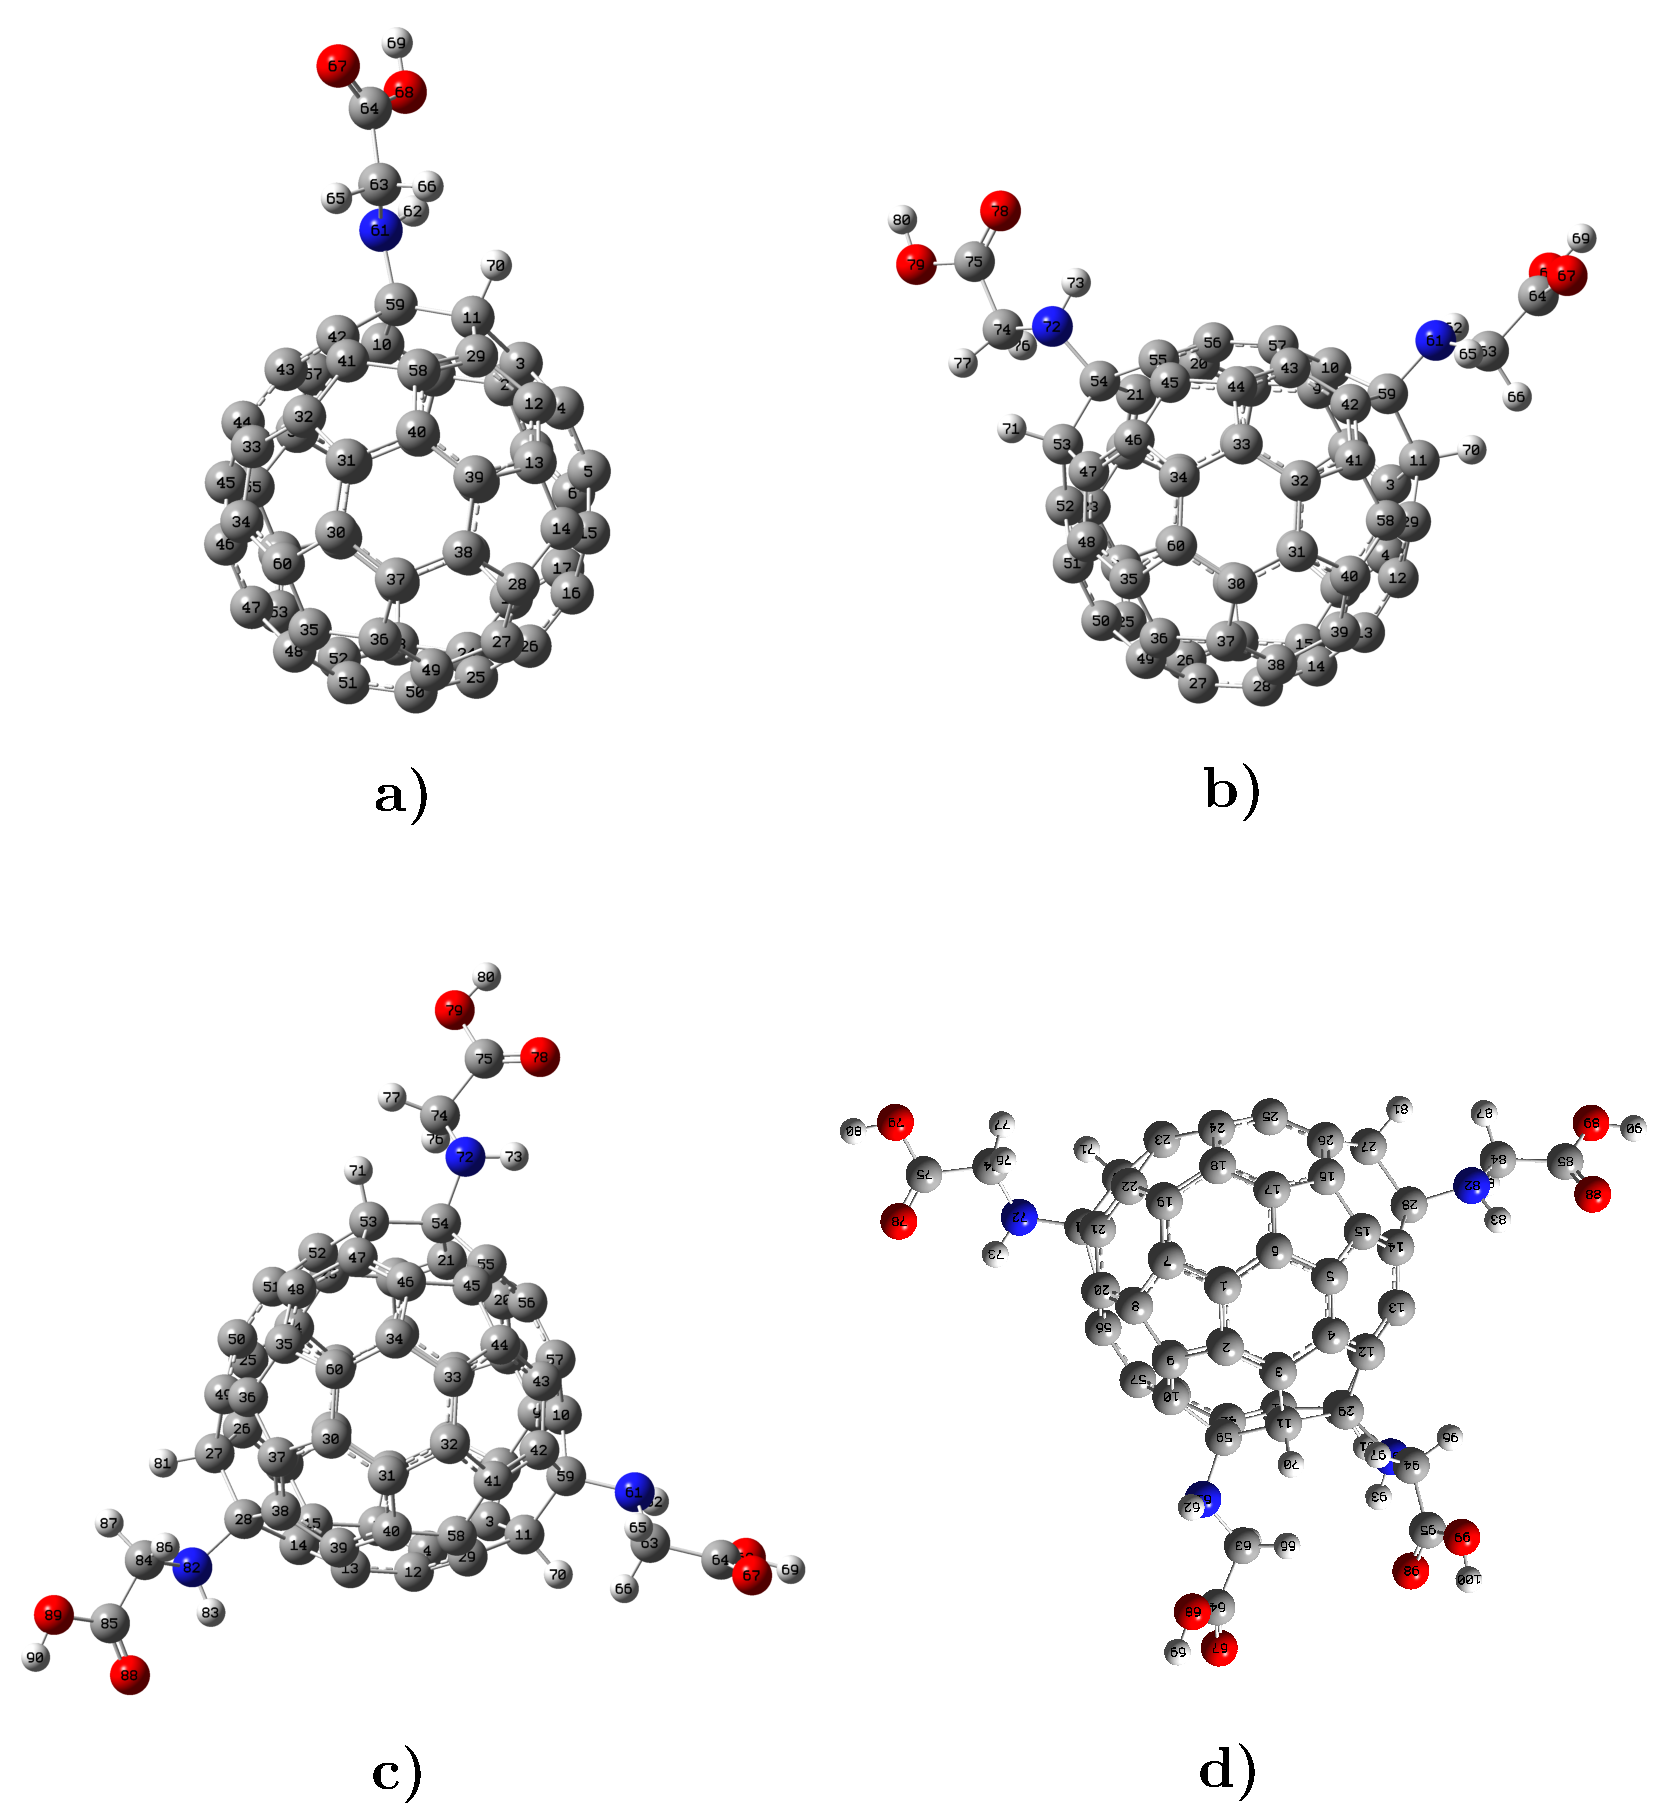
\includegraphics[width=1.0\textwidth]{imagenes/Resu/opt-gly-4.pdf}
      \caption{Estructuras optimizadas de los isómeros evaluados para la segunda adición de glicina al sistema  C\textsubscript{60}(Gly). Los paneles (a)--(d) corresponden a las alternativas estructurales comparadas en esta etapa.}
      \label{fig:isomeros-gly2}
        \end{figure}

        
Para determinar la viabilidad termodinámica y la reactividad de la primera adición de glicina sobre la jaula del C\textsubscript{60}, se llevaron a cabo cálculos de optimización de geometría y análisis de frecuencias vibracionales empleando la teoría del funcional de la densidad (DFT) con el funcional híbrido B3LYP y el conjunto de bases 6-311G(d,p). La ausencia de frecuencias imaginarias en los cálculos confirmó que todas las estructuras corresponden a mínimos locales en la superficie de energía potencial. Adicionalmente, se determinaron las funciones de Fukui para evaluar la reactividad electrofílica y nucleofílica local de la jaula.

Debido a la alta simetría icosaédrica del C\textsubscript{60} prístino, los 60 átomos de carbono son químicamente equivalentes previo a la reacción. Por lo tanto, en todas las propuestas evaluadas la molécula de glicina se ancló sobre el carbono C59, variando la posición de adición del átomo de hidrógeno complementario para mapear la regioquímica del sistema  \textbf{veáse Figura~\ref{fig:isomeros-gly2}}:


\section{Análisis de descriptores de reactividad global (PI y AE)}

Con el propósito de evaluar los cambios en las propiedades electrónicas del fulereno después de su funcionalización con glicina, se analizaron el potencial de ionización (PI) y la afinidad electrónica (AE) del C\textsubscript{60} prístino y del sistema tetrafuncionalizado C\textsubscript{60}(Gly)\textsubscript{4}. Estos parámetros permiten comparar la energía necesaria para remover un electrón y la tendencia energética de cada estructura a aceptar un electrón, respectivamente. Los valores obtenidos se presentan en la Tabla~\ref{tab:energias-referencia}.

\begin{table}[H]
    \centering
    \caption{Potencial de ionización (PI) y afinidad electrónica (AE), en eV, del fulereno C\textsubscript{60} y del aducto C\textsubscript{60}(Gly)\textsubscript{4}.}
    \label{tab:energias-referencia}
    \renewcommand{\arraystretch}{1.15}
    \begin{tabular}{lcc}
        \toprule
        \textbf{Sistema} & \textbf{PI (eV)} & \textbf{AE (eV)} \\
        \midrule
        Fulereno C\textsubscript{60} & 7.608 & 2.454 \\
        C\textsubscript{60}(Gly)\textsubscript{4} & 6.849 & 1.779 \\
        \bottomrule
    \end{tabular}
\end{table}

Como se observa en la Tabla~\ref{tab:energias-referencia}, el potencial de ionización disminuye de 7.608 eV en el C\textsubscript{60} prístino a 6.849 eV en el sistema C\textsubscript{60}(Gly)\textsubscript{4}, lo que representa una diferencia de 0.759 eV. Esta disminución indica que la extracción de un electrón requiere menos energía en el derivado funcionalizado. Por lo tanto, la incorporación de cuatro grupos de glicina modifica las propiedades electrónicas de la jaula y favorece, desde el punto de vista energético, la pérdida de un electrón respecto al fulereno sin funcionalizar.

Por su parte, la afinidad electrónica presenta una disminución de 2.454 a 1.779 eV, equivalente a 0.675 eV. Este resultado indica que el sistema tetrafuncionalizado tiene una menor tendencia energética a aceptar un electrón en comparación con el C\textsubscript{60} prístino. En conjunto, ambos parámetros muestran que la incorporación de glicina modifica la respuesta electrónica del fulereno, disminuyendo tanto la energía necesaria para su ionización como la afinidad por un electrón adicional.

Estos cambios son relevantes debido a que la capacidad de donar o aceptar electrones puede intervenir en procesos de transferencia electrónica asociados con sistemas biológicos. En particular, la disminución del potencial de ionización sugiere que el derivado tetrafuncionalizado podría participar con mayor facilidad en procesos de donación electrónica. Sin embargo, esta característica no permite establecer por sí sola una actividad antioxidante, ya que dicha propiedad también depende de la naturaleza de las especies reactivas, del medio y de los mecanismos involucrados.

De esta manera, los resultados indican que la funcionalización con glicina no solamente modifica la estructura del C\textsubscript{60}, sino también sus propiedades electrónicas globales. Además, la incorporación de grupos funcionales polares, como los grupos amino y carboxilo, introduce nuevos sitios de interacción que podrían influir en su comportamiento en medios acuosos y en el reconocimiento molecular. Para complementar este análisis, se evaluó la distribución del potencial electrostático de los sistemas obtenidos durante las distintas etapas de funcionalización.


\section{Potencial electrostático superficial}

Con la finalidad de analizar cómo cambia la distribución electrostática del fulereno conforme aumenta el número de grupos de glicina, se evaluaron los sistemas C\textsubscript{60}, C\textsubscript{60}(Gly), C\textsubscript{60}(Gly)\textsubscript{2}, C\textsubscript{60}(Gly)\textsubscript{3} y C\textsubscript{60}(Gly)\textsubscript{4}. El análisis se realizó mediante los valores de potencial electrostático obtenidos con el programa Multiwfn. Los resultados promedio correspondientes a cada estructura se presentan en la Tabla~\ref{tab:potencial-electrostatico}.

\begin{table}[H]
    \centering
    \caption{Valores promedio de potencial electrostático para el fulereno C\textsubscript{60} y los sistemas funcionalizados con una a cuatro moléculas de glicina.}
    \label{tab:potencial-electrostatico}
    \renewcommand{\arraystretch}{1.15}
    \begin{tabular}{lc}
        \toprule
        \textbf{Sistema} & \textbf{Potencial electrostático promedio} \\
        \midrule
        Fulereno C\textsubscript{60} & 1.465 \\
        C\textsubscript{60}(Gly) & 0.975 \\
        C\textsubscript{60}(Gly)\textsubscript{2} & 2.289 \\
        C\textsubscript{60}(Gly)\textsubscript{3} & 2.556 \\
        C\textsubscript{60}(Gly)\textsubscript{4} & 6.024 \\
        \midrule
        \textbf{Promedio} & \textbf{2.662} \\
        \bottomrule
    \end{tabular}
\end{table}

Los valores de la Tabla~\ref{tab:potencial-electrostatico} muestran que la incorporación de glicina modifica el potencial electrostático promedio del sistema. El fulereno prístino presenta un valor de 1.465, mientras que la primera adición de glicina produce una disminución hasta 0.975. Sin embargo, a partir de la segunda incorporación se observa un incremento progresivo, con valores de 2.289 y 2.556 para los sistemas con dos y tres grupos de glicina, respectivamente, hasta alcanzar 6.024 en el derivado tetrafuncionalizado.

Este comportamiento indica que la variación del potencial electrostático no es uniforme durante todas las etapas de funcionalización. Aunque la primera adición disminuye el valor promedio, las incorporaciones posteriores producen un desplazamiento hacia valores más positivos. En particular, el sistema C\textsubscript{60}(Gly)\textsubscript{4} presenta el mayor potencial promedio entre las estructuras evaluadas, con un valor aproximadamente cuatro veces superior al del fulereno prístino. Esta diferencia sugiere que la presencia y distribución de los grupos de glicina influyen de manera importante en las características electrostáticas del sistema.

Para examinar con mayor detalle este comportamiento, en la Figura~\ref{fig:esp-promedio} se presenta la distribución de los valores de potencial electrostático asociados con los sitios atómicos de cada estructura. A diferencia de los valores promedio, esta representación permite identificar las regiones que presentan contribuciones positivas y negativas, así como los cambios que ocurren durante las adiciones sucesivas de glicina.

\begin{figure}[H]
    \centering
    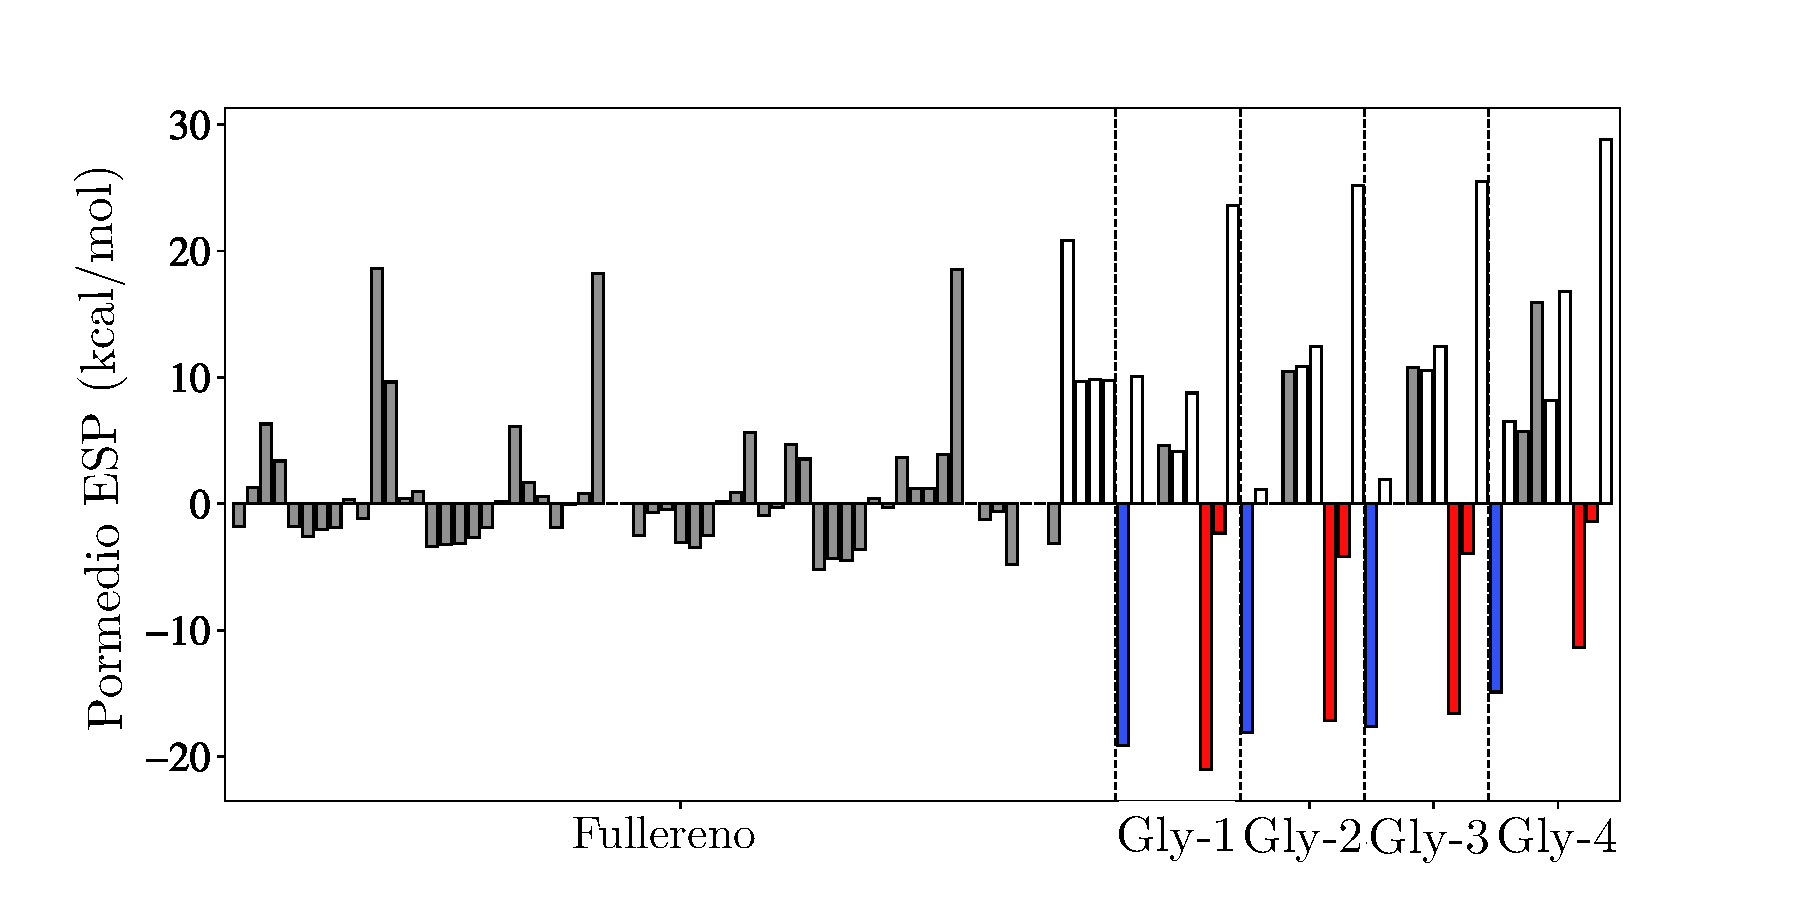
\includegraphics[width=1.0\textwidth]{imagenes/Resu/figure_2.pdf}
    \caption{Distribución de los valores de potencial electrostático asociados con los sitios atómicos del fulereno C\textsubscript{60} y de los sistemas funcionalizados con una a cuatro moléculas de glicina. Las líneas verticales discontinuas separan los sistemas analizados.}
    \label{fig:esp-promedio}
\end{figure}

Como se observa en la Figura~\ref{fig:esp-promedio}, los valores correspondientes a los átomos de carbono del fulereno prístino se distribuyen principalmente alrededor de cero, aunque algunos sitios presentan desviaciones positivas. Después de la incorporación de glicina, la distribución se amplía y aparecen regiones con valores positivos y negativos de mayor magnitud. Este comportamiento se relaciona con la presencia de átomos de distinta electronegatividad y con la redistribución de la densidad electrónica alrededor de los grupos funcionales incorporados.

Los valores más negativos se encuentran principalmente asociados con los átomos de oxígeno y nitrógeno de los sustituyentes, con contribuciones que se aproximan a -20 kcal mol$^{-1}$. Por el contrario, algunos átomos de hidrógeno presentan valores positivos superiores a 20 kcal mol$^{-1}$. Esta diferencia permite distinguir regiones con características electrostáticas opuestas dentro de una misma estructura. Asimismo, se observa que la incorporación sucesiva de glicina aumenta el número de sitios con contribuciones electrostáticas diferenciadas, especialmente en los sistemas con tres y cuatro sustituyentes.

La coexistencia de estas regiones indica que, aunque el potencial promedio aumenta durante las últimas etapas de funcionalización, la superficie molecular no adquiere un carácter uniformemente positivo. Por el contrario, conserva zonas con distinta distribución electrostática, lo que podría favorecer interacciones de diferente naturaleza con otras moléculas. Para observar espacialmente estas regiones, se analizó el mapa de potencial electrostático molecular del sistema C\textsubscript{60}(Gly)\textsubscript{4}, presentado en la Figura~\ref{fig:mep-gly4}.

\begin{figure}[H]
    \centering
    \includegraphics[width=1.0\textwidth]{imagenes/Resu/figure_5.png}
    \caption{Mapa de potencial electrostático molecular del sistema C\textsubscript{60}(Gly)\textsubscript{4} observado desde dos orientaciones. Los colores representan regiones de potencial negativo (rojo), cercano a cero (verde) y positivo (azul).}
    \label{fig:mep-gly4}
\end{figure}

En la Figura~\ref{fig:mep-gly4} se observa que las regiones de potencial electrostático negativo, representadas en rojo, se localizan principalmente alrededor de los átomos de oxígeno de los grupos carboxilo. Por su parte, las regiones positivas, identificadas en azul, se encuentran próximas a determinados átomos de hidrógeno de los sustituyentes. La superficie de la jaula de C\textsubscript{60} conserva principalmente tonalidades verdes, correspondientes a valores cercanos a cero dentro de la escala empleada. Esta distribución confirma que la incorporación de glicina genera una superficie electrostáticamente heterogénea, sin eliminar las características del núcleo carbonoso.

La presencia simultánea de regiones positivas, negativas y cercanas a cero resulta de interés para el reconocimiento molecular, debido a que permite considerar diferentes posibilidades de interacción con una proteína. Las zonas de potencial negativo podrían participar en interacciones con regiones electropositivas o actuar como sitios aceptores de puentes de hidrógeno, mientras que las regiones de potencial positivo podrían favorecer interacciones con grupos electronegativos. Asimismo, la superficie carbonosa del fulereno podría contribuir a contactos de dispersión y a interacciones con regiones poco polares.

En relación con la posible interacción del sistema C\textsubscript{60}(Gly)\textsubscript{4} con proteínas del virus del dengue, estos resultados proporcionan información sobre las características electrostáticas del ligando que podrían intervenir en el reconocimiento molecular. No obstante, la distribución de potencial observada no permite establecer por sí sola la afinidad, la estabilidad ni la especificidad de una interacción con la proteína NS2B-NS3. Para determinar estas características es necesario considerar también la distribución electrostática de la proteína, la geometría del sitio de unión y los resultados de los estudios de acoplamiento molecular.

En conjunto, los resultados muestran que la funcionalización secuencial con glicina modifica tanto las propiedades electrónicas globales como la distribución electrostática superficial del fulereno. La disminución del potencial de ionización y de la afinidad electrónica, junto con la aparición de regiones electrostáticas diferenciadas, indica que la incorporación de los sustituyentes modifica las posibilidades de interacción del sistema. Estas características constituyen una base para analizar posteriormente su comportamiento frente a la diana biológica seleccionada.
\section{Estructura de la proteína NS2B-NS3}  
La proteasa NS2B/NS3 del serotipo 2 del virus del dengue (DENV-2), con una masa molecular de $26.57\ \text{kDa}$, representa un blanco terapéutico primordial por su papel clave en la replicación viral. Al evaluar el modelo en conformación abierta e inactiva reconstruido en sus regiones desordenadas mediante AlphaFold, se observa que la estructura presenta una alta fidelidad conformacional.

En el mapa de Ramachandran se aprecia una distribución óptima de los ángulos diedros ($\phi, \psi$), donde la gran mayoría de los residuos se ubican en zonas energéticamente favorecidas. A partir de esta base estructural, los $100\ \text{ns}$ de dinámica molecular (MD) bajo el campo de fuerzas CHARMM36 reflejan la respuesta conformacional y la estabilidad del sistema en solución acuosa.



%
%\begin{table}[htbp]
%\centering
%\caption{Cuadrantes del Diagrama de Ramachandran}
%\vspace{0.3cm}
%\begin{tabularx}{\textwidth}{p{3cm} p{3.2cm} X}
%\toprule
%\textbf{Cuadrante} & \textbf{Rango de Ángulos} & \textbf{Significado y Estructuras Comunes} \\
%\midrule
%\textbf{Superior izquierdo (NW)} & $\phi$ negativo, $\psi$ positivo & \textbf{La zona más poblada.} Aquí se encuentran las \textbf{láminas beta} ($\beta$-sheets) y las estructuras extendidas. Los aminoácidos están cómodos porque sus cadenas laterales apuntan en direcciones opuestas al esqueleto. \\
%\addlinespace
%\textbf{Inferior izquierdo (SW)} & $\phi$ negativo, $\psi$ negativo & \textbf{Zona de las hélices alfa derechas ($\alpha$-helices).} Es una región altamente favorecida donde la cadena se enrolla de forma natural y compacta. \\
%\addlinespace
%\textbf{Superior derecho (NE)} & $\phi$ positivo, $\psi$ positivo & \textbf{Zona de las hélices alfa izquierdas.} Es una estructura muy rara en proteínas naturales; casi ningún aminoácido del "caso general" puede entrar aquí debido a choques atómicos. \\
%\addlinespace
%\textbf{Inferior derecho (SE)} & $\phi$ positivo, $\psi$ blanco/negativo & \textbf{Zona prohibida casi por completo.} Es energéticamente imposible para casi todos los aminoácidos debido a colisiones frontales extremas entre sus átomos. \\
%\bottomrule
%\end{tabularx}
%\end{table}
%\clearpage

\begin{figure}[H]
    \centering
    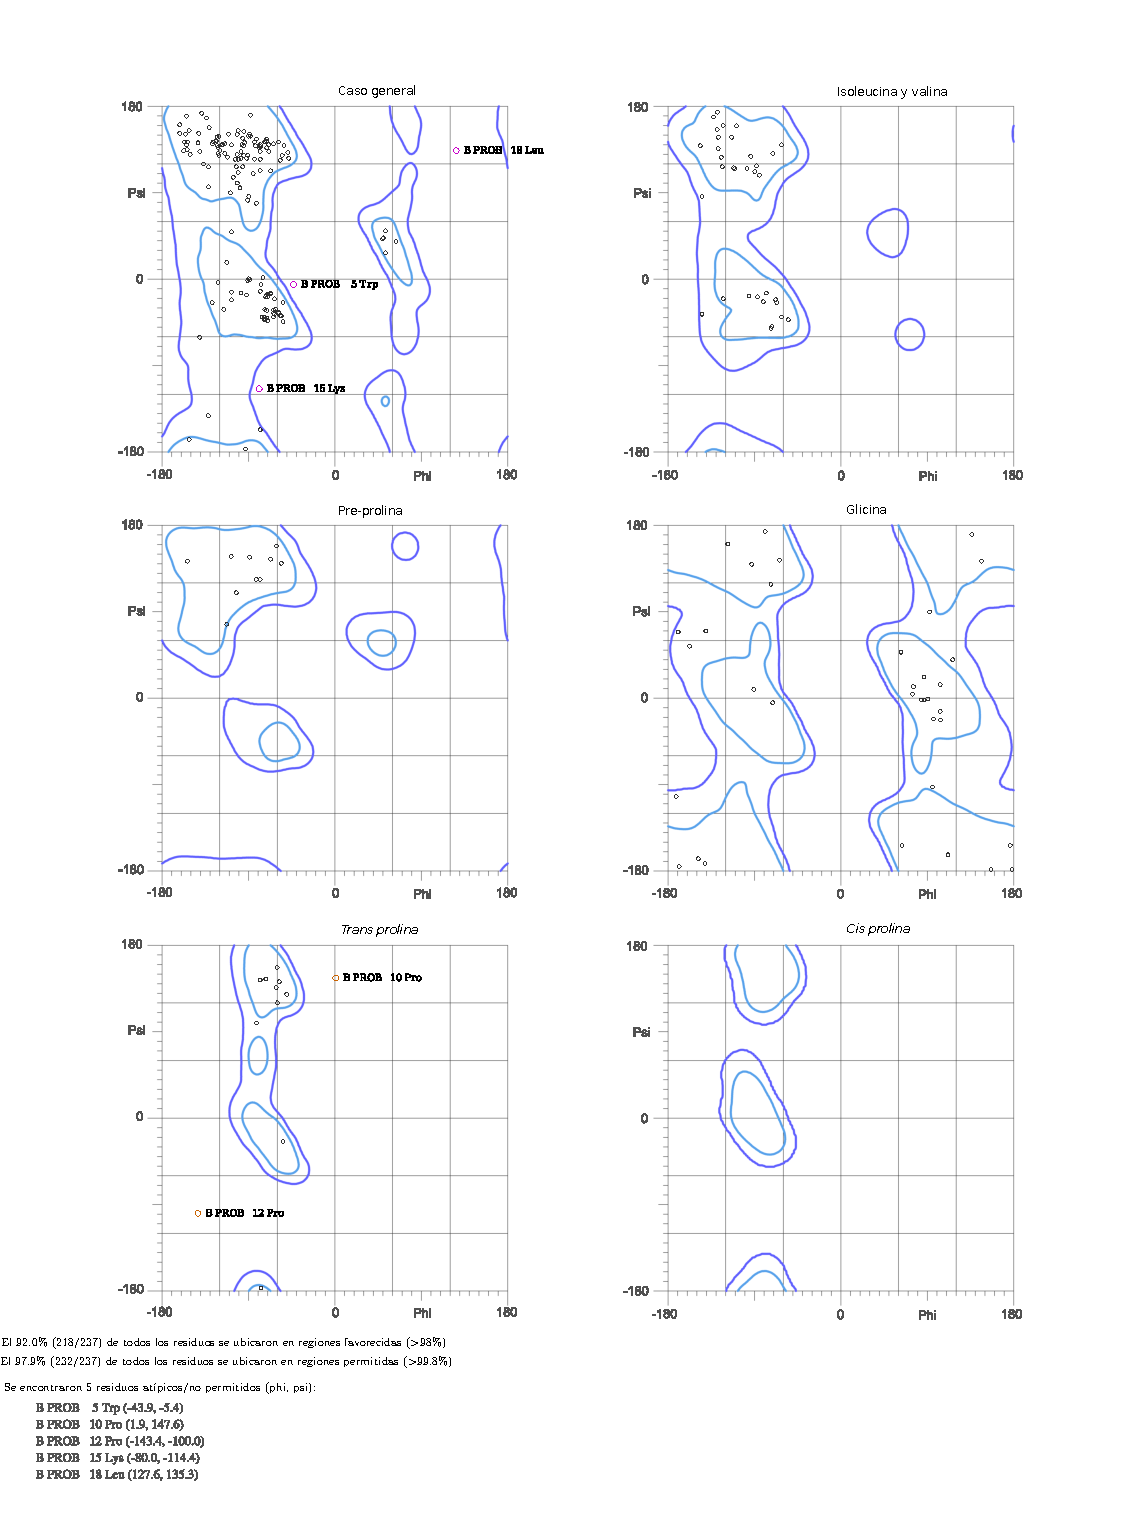
\includegraphics[width=0.95\textwidth]{imagenes/Resu/2FOM_original-rama.pdf}
    \caption{Diagramas de Ramachandran (MolProbity) para la estructura proteica inicial. Evaluación de la calidad estereoquímica del modelo nativo antes de los procesos de minimización de energía.} 
    \label{fig:ramachandra}
\end{figure}
\newpage
El gráfico de Ramachandran constituye una herramienta fundamental para evaluar la calidad estereoquímica de las estructuras proteicas. Mediante la representación de las combinaciones posibles de los ángulos diédricos $\phi$ (phi) y $\psi$ (psi) del esqueleto peptídico, es posible determinar a priori las conformaciones secundarias adoptadas (principalmente $\alpha$-hélices y láminas $\beta$), así como validar la fiabilidad física de la estructura tridimensional.

En la Figura~\ref{fig:ramachandra} se presenta el análisis estereoquímico obtenido con MolProbity para el estado inicial sin la dinamica de la NS2B-NS3. De manera global, el 92.0\% de los residuos (218/237) se ubicaron en regiones favorecidas y el 97.9\% (232/237) en regiones permitidas. Aunque la estructura presenta una calidad geométrica general adecuada, se identificaron 5 residuos atípicos fuera de las regiones conformacionales permitidas (2.1\% de atípicos), representados por sus ángulos de torsión ($\phi$, $\psi$): Trp5 ($-43.9^\circ, -5.4^\circ$), Lys15 ($-80.0^\circ, -114.4^\circ$) y Leu18 ($127.6^\circ, 135.3^\circ$) en el panel general, así como Pro10 ($1.9^\circ, 147.6^\circ$) y Pro12 ($-143.4^\circ, -100.0^\circ$) en la categoría de \textit{trans}-prolina. La presencia de estos residuos fuera de los límites geométricos aceptables evidencia la existencia de impedimentos estéricos o tensiones conformacionales locales en el estado cristalográfico o de partida, las cuales se espera que se relajen durante la fase de minimización y simulación de dinámica molecular.

La diferenciación en los paneles del análisis responde a las particularidades fisicoquímicas y estructurales de los distintos aminoácidos:

\begin{itemize}
    \item \textbf{Caso general y glicina:} El gráfico general contempla los aminoácidos con cadenas laterales estándar. Por el contrario, la glicina se analiza en una parcela independiente debido a que carece de cadena lateral (posee solo un átomo de hidrógeno como radical), lo que le otorga una flexibilidad conformacional significativamente mayor y le permite adoptar combinaciones de ángulos $\phi$ y $\psi$ en regiones que serían prohibidas para el resto de los residuos por impedimento estérico.
    \item \textbf{Isoleucina y valina:} Presentan un espacio conformacional más restringido debido a la ramificación en el carbono beta ($\text{C}_\beta$), situada muy próxima al esqueleto peptídico, lo que limita los grados de libertad rotacionales. En el modelo analizado, la totalidad de los residuos de Isoleucina y Valina se ubicaron dentro de las regiones permitidas.
    \item \textbf{Prolina y pre-prolina:} La prolina posee un anillo de pirrolidina rígido que conecta la cadena lateral con el nitrógeno del enlace amida, fijando fuertemente el ángulo $\phi$ en valores cercanos a $-60^\circ$. Por su parte, las regiones de pre-prolina (residuos inmediatamente anteriores a una prolina) también se ven restringidos por su espacio conformacional por el volumen estérico del anillo subsiguiente. En nuestro sistema, mientras que el grupo de pre-prolina y \textit{cis}-prolina no mostró anomalías, el subgrupo de \textit{trans}-prolina concentró dos de los desfases geométricos identificados (Pro10 y Pro12).
\end{itemize}


\begin{figure}[H]
    \centering
    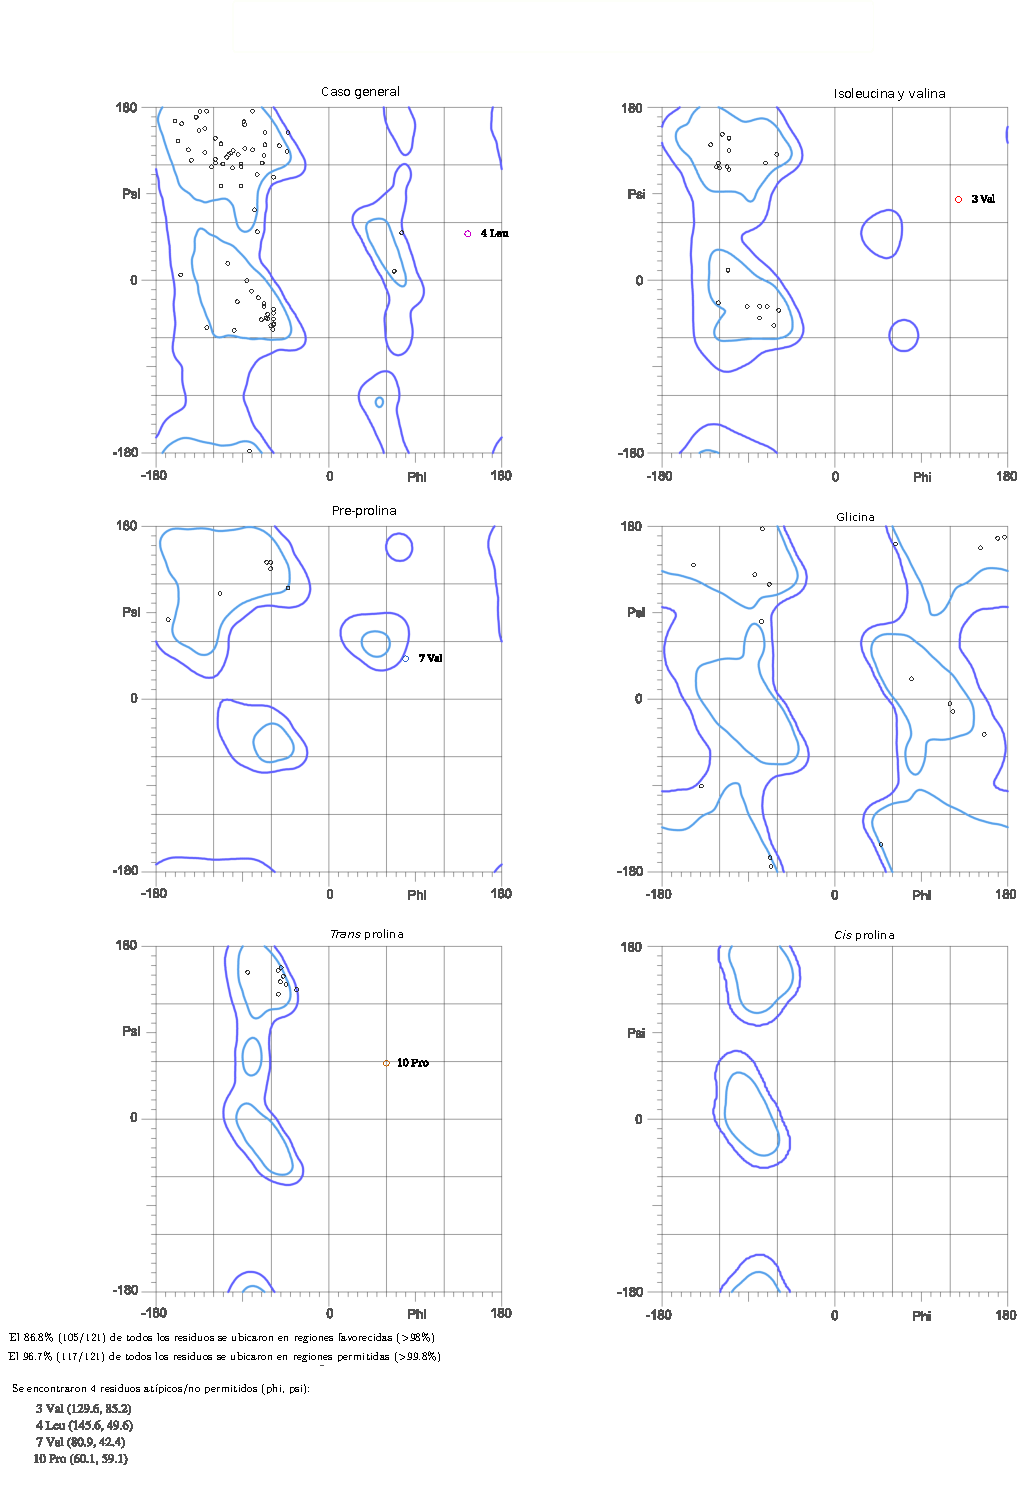
\includegraphics[width=0.85\textwidth]{imagenes/Resu/2FOM_post_npt1-rama.pdf}
    \caption{Diagramas de Ramachandran (MolProbity) tras el equilibrio NPT. Evaluación de la calidad estereoquímica de la estructura proteica al finalizar la etapa de equilibrio isotérmico-isobárico (NPT), previa a la fase de producción de dinámica molecular.} 
    \label{fig:ramachandra-2}
\end{figure}
El análisis de Ramachandran posterior a la etapa de equilibrio en el ensamble isotérmico-isobárico, refleja una clara \textbf{recuperación y relajación estereoquímica} de la estructura proteica tras el impacto inicial de la minimización (Figura~\ref{fig:ramachandra-2}). La proporción de residuos en regiones favorecidas se incrementó del 84.3\% al \textbf{86.8\%} (105/121 residuos), mientras que los residuos en regiones permitidas ascendieron del 92.6\% al \textbf{96.7\%} (117/121 residuos). De forma consistente, el número total de residuos atípicos fuera de los límites geométricos se redujo notablemente de 9 a solo **4 residuos** (3.3\% del total de la estructura recortada).

Esta mejora cuantitativa demuestra que la introducción de la temperatura y la presión durante la fase NPT otorgó la energía térmica suficiente al sistema para superar las trampas cinéticas locales generadas en la minimización, permitiendo que el esqueleto peptídico rotara hacia mínimos de energía conformacional más favorables.

El detalle de los 4 residuos atípicos ($\phi, \psi$) identificados en los distintos cuadrantes es el siguiente:

\begin{itemize}
    \item \textbf{Caso general:} Se registró a \textbf{4 Leu} ($145.6^\circ, 49.6^\circ$) fuera del área permitida, ubicándose en el cuadrante superior derecho (zona de hélices izquierdas no nativas).
    \item \textbf{Isoleucina y valina:} Se identificó a \textbf{3 Val} ($129.6^\circ, 85.2^\circ$) desplazado hacia la región superior derecha fuera del mapa permitido para residuos $\beta$-ramificados.
    \item \textbf{Pre-prolina:} El residuo \textbf{7 Val} ($80.9^\circ, 42.4^\circ$) se mantiene fuera de los límites aceptados, reflejando una restricción torsional impuesta por la cercanía al segmento rico en prolinas.
    \item \textbf{Trans-prolina:} A diferencia de la minimización previa donde se acumulaban cuatro prolinas distorsionadas (Pro8, Pro10, Pro11 y Pro12), tras el equilibrio NPT solo se conserva a \textbf{10 Pro} ($60.1^\circ, 59.1^\circ$) fuera del intervalo permitido. Las demás prolinas relajaron sus ángulos diédricos y retornaron exitosamente a las regiones estereoquímicamente permitidas.
\end{itemize}

Un aspecto estructural relevante es que los 4 residuos fuera de la conformación idónea (Val3, Leu4, Val7 y Pro10) se encuentran agrupados secuencialmente en el extremo N-terminal del fragmento. Esto sugiere que el núcleo de la proteína ha alcanzado una conformación estable y bien empaquetada, quedando la tensión residual concentrada exclusivamente en un bucle o segmento flexible N-terminal. En conclusión, la equilibración NPT1 cumplió de forma efectiva con la reordenación del esqueleto peptídico, preparando un punto de partida físicamente estable para la dinámica de producción.
\subsection{Comportamiento de la estabilidad global y movilidad (RMSD)}

Al analizar la evolución de la raíz de la desviación cuadrática media (RMSD) de los átomos $C\alpha$ Figura~\ref{fig:rmsd-2fom}, se observa un incremento inicial rápido durante los primeros $5\ \text{ns}$ hasta alcanzar $\sim 0.40\ \text{nm}$, lo cual se atribuye a la acomodación y relajación inicial del sistema en el entorno de solvatación.

Entre los $10$ y $40\ \text{ns}$, la trayectoria exhibe un régimen de equilibrio relativo en torno a $0.40 - 0.45\ \text{nm}$. Sin embargo, entre los $45 - 55\ \text{ns}$ y $75 - 85\ \text{ns}$, se detectan fluctuaciones más marcadas que alcanzan picos de hasta $0.65\ \text{nm}$. Estas variaciones no responden a un proceso de desnaturalización, sino a la notable movilidad intrínseca de la proteína en su estado abierto e inactivo, asociada a los reordenamientos del bucle cofactórico de NS2B y del dominio catalítico. La posterior estabilización del RMSD en la franja de $0.40 - 0.45\ \text{nm}$ durante los últimos $15\ \text{ns}$ confirma que el sistema de estabilizo en una región de energía potencial mínima. 

                

\begin{figure}[H]
    \centering
    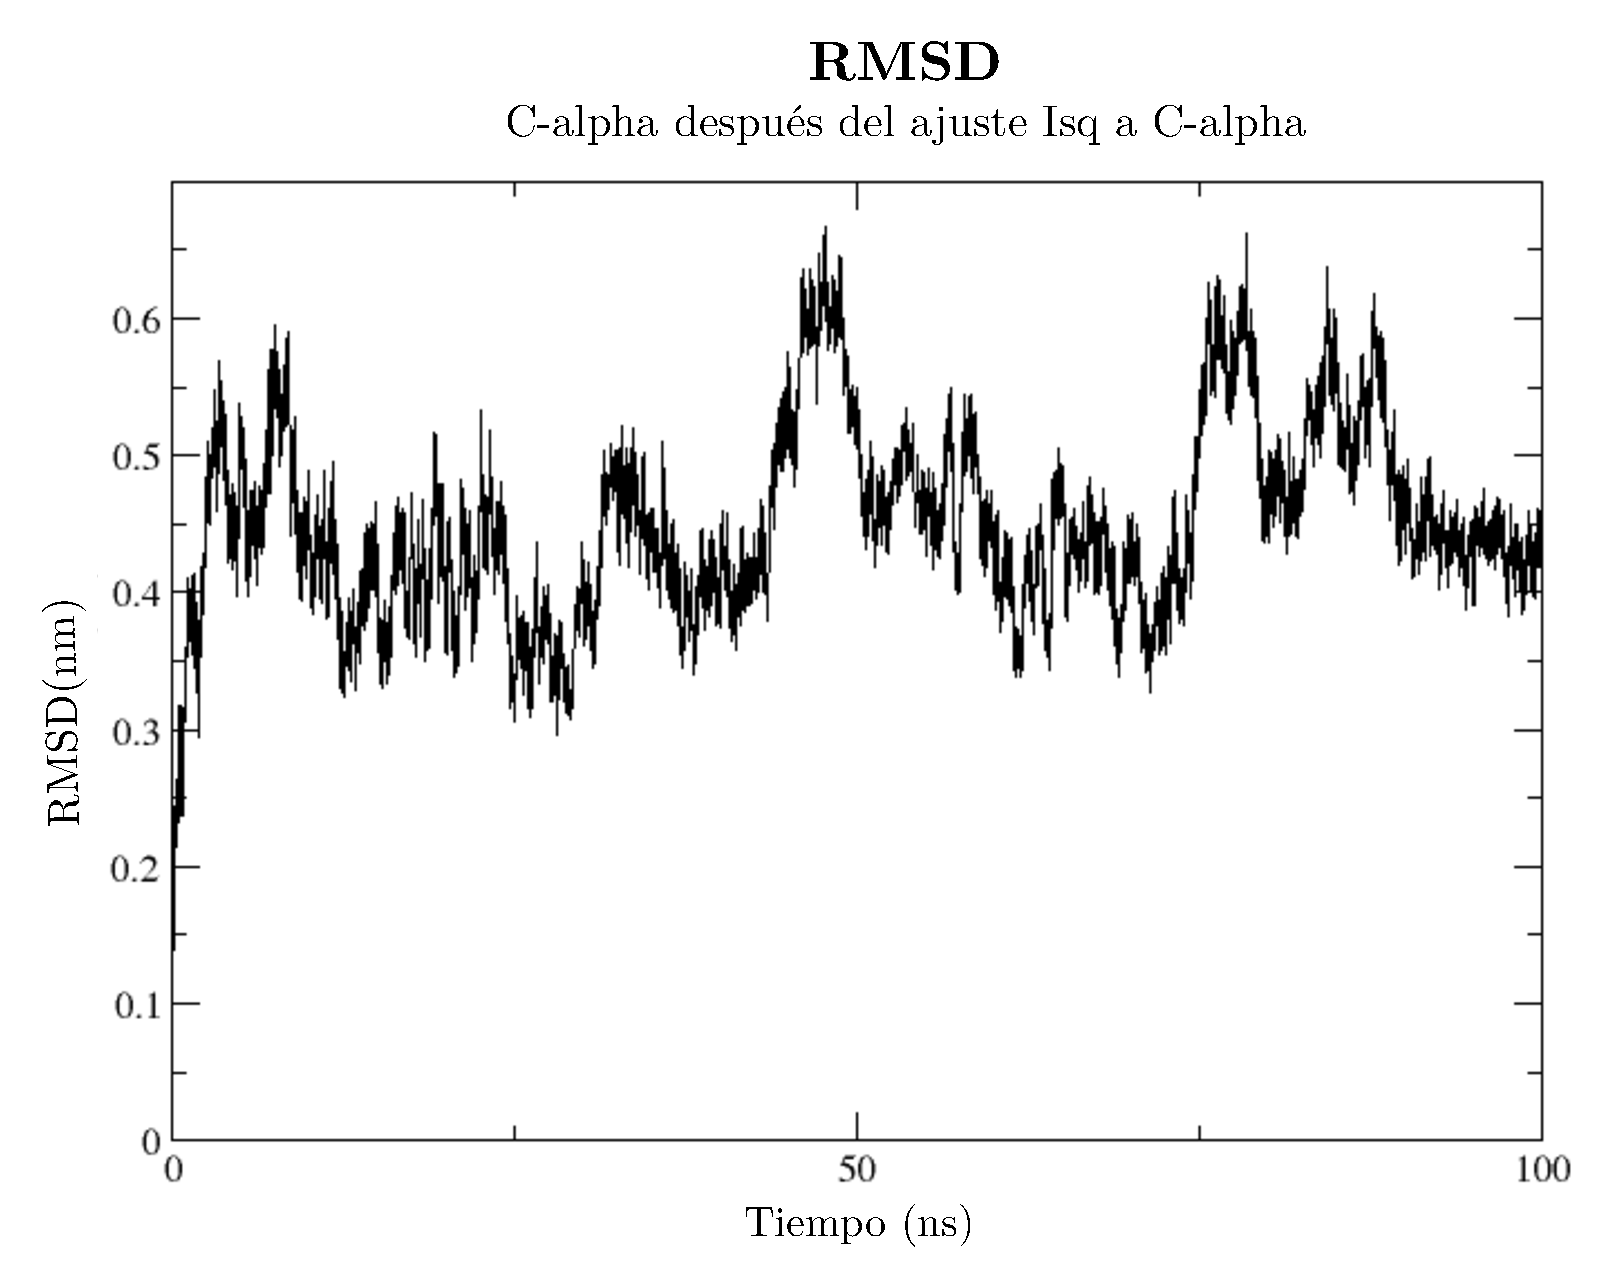
\includegraphics[width=0.82\textwidth]{imagenes/Resu/rmsd-2.pdf}
    \caption{Evolución del RMSD de los átomos C$\alpha$ de la proteína, durante 100 ns de dinámica molecular.}
    \label{fig:rmsd-2fom}
\end{figure}


\subsection{Proceso de compactación y exposición hidrofóbica ($R_g$ y SASA)}

Los perfiles del Radio de Giro ($R_g$) y del Área Superficial Accesible al Solvente (SASA) (Figura~\ref{fig:rg-sasa-2fom}) respaldan esta interpretación y aportan información sobre el comportamiento macroestructural:

\begin{itemize}
    \item \textbf{Radio de giro ($R_g$):} A partir del valor inicial de $1.90\ \text{nm}$, se aprecia una expansión transitoria hasta $1.97\ \text{nm}$ en los primeros $15\ \text{ns}$, producto de la apertura de bucles flexibles. No obstante, a partir del nanosegundo $20$ se identifica una tendencia continua hacia la compactación que alcanza un mínimo de $1.82\ \text{nm}$ hacia los $50\ \text{ns}$, para posteriormente mantenerse constante entre $1.84$ y $1.88\ \text{nm}$. Este comportamiento demuestra que la proteína tiende hacia un empaquetamiento más globular con el paso del tiempo.
    
    \item \textbf{Área accesible al solvente (SASA):} En concordancia con la contracción del $R_g$, se observa una disminución clara en el SASA total desde $\sim 155\ \text{nm}^2$ hasta fluctuar en la franja de $145 - 150\ \text{nm}^2$. Esta reducción refleja la ocurrencia de un colapso hidrofóbico interno que minimiza la exposición de los residuos apolares al solvente.
\end{itemize}
        
\begin{figure}[H]
    \centering
    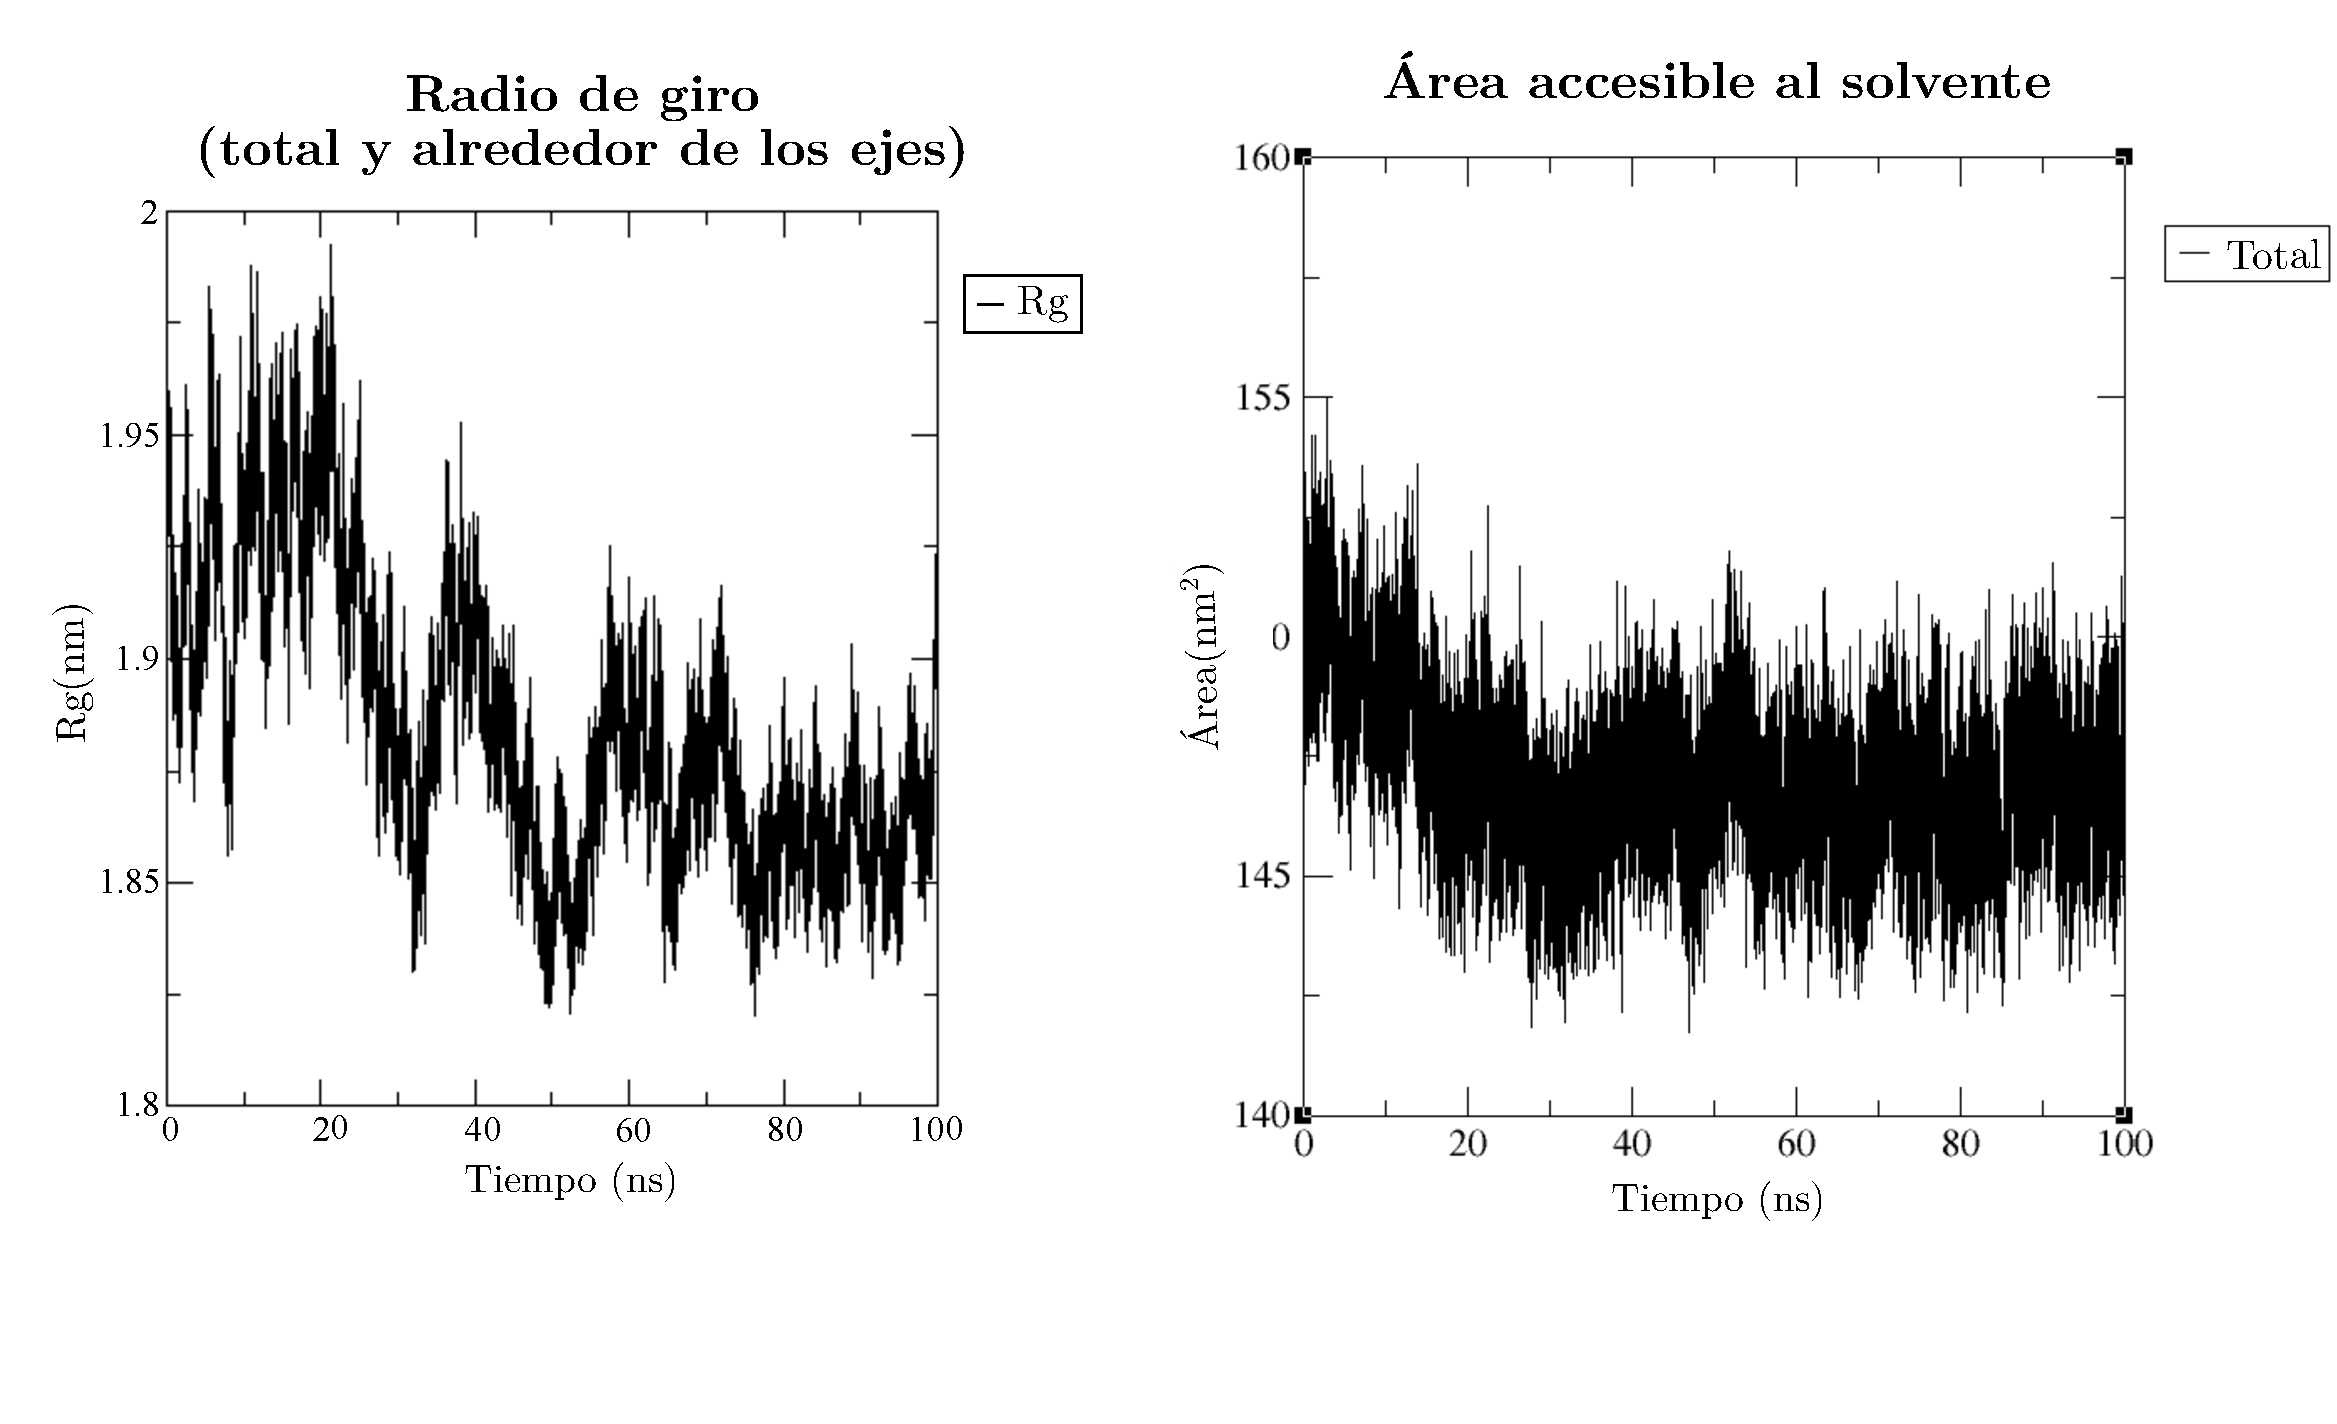
\includegraphics[width=0.95\textwidth]{imagenes/Resu/radio.pdf}
    \caption{Evolución temporal del radio de giro ($R_g$) y del área superficial accesible al solvente (SASA) durante los 100 ns de trayectoria de dinámica molecular.}
    \label{fig:rg-sasa-2fom}
\end{figure} 

\subsection{Dinámica de la red interna de enlaces de hidrógeno}

Al examinar la red de enlaces de hidrógeno intramoleculares (Figura~\ref{fig:hbond-2fom}), se encuentra la explicación molecular a la compactación observada. Se evidencia que la proteasa mantiene de forma constante entre $130$ y $150$ enlaces de hidrógeno internos a lo largo de toda la trayectoria. Destaca un incremento notable en la densidad de estas interacciones entre los $40$ y $60\ \text{ns}$ (con picos de hasta $\sim 165$ contactos), coincidiendo de manera exacta con el mínimo observado en el Radio de Giro ($R_g \approx 1.82\ \text{nm}$).

Este comportamiento demuestra que el fortalecimiento de la red electrostática interna actuó como la fuerza impulsora que consolidó la estructura terciaria frente a la movilidad de los bucles.

En conclusión, la consistencia observada entre la estabilización del RMSD ($\sim 0.42\ \text{nm}$), la reducción del $R_g$ ($1.85\ \text{nm}$), la disminución del SASA ($146\ \text{nm}^2$) y la preservación continua de la red de enlaces de hidrógeno intramoleculares permite concluir que la proteasa DENV-2 en conformación abierta e inactiva alcanza una marcada estabilidad estructural bajo las condiciones simuladas.

\begin{figure}[H]
    \centering
    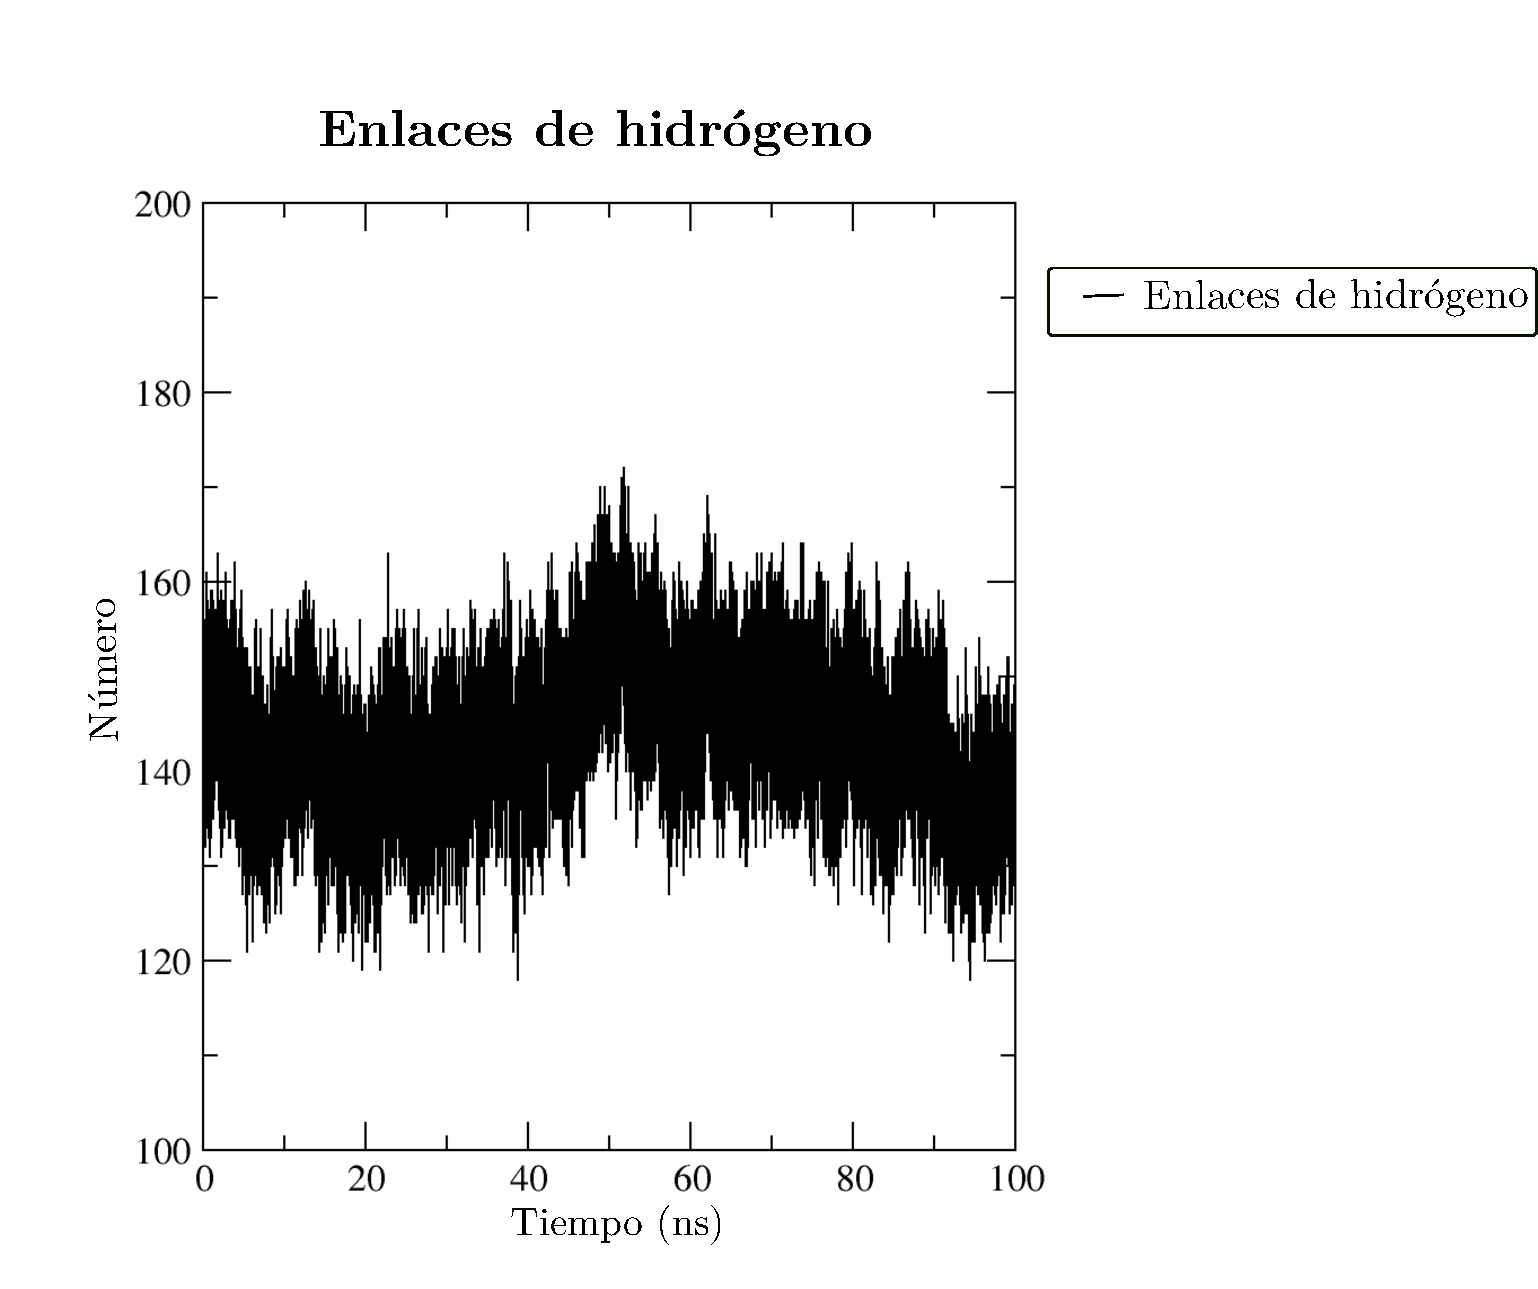
\includegraphics[width=0.70\textwidth]{imagenes/Resu/hidrogeno.pdf}
    \caption{Evolución temporal del número de enlaces de hidrógeno intramoleculares formados en la proteína a lo largo de 100 ns.}
    \label{fig:hbond-2fom}
\end{figure}  


Con el propósito de evaluar la afinidad de unión y el comportamiento conformacional de distintos sistemas de ligandos frente a diferentes regiones de la proteína —incluyendo tanto el sitio ortostérico como posibles sitios alostéricos—, se llevaron a cabo ensayos de acoplamiento molecular (docking) mediante el programa AutoDock Vina. Como ejemplo de estas evaluaciones, en la (Figura~\ref{fig:benzamida-3d}) se muestra la pose conformacional de menor energía obtenida para uno de los sistemas, destacando la red de interacciones no covalentes (como puentes de hidrógeno y contactos de tipo $\pi$) en el sitio de unión. 

\begin{figure}[H]
      \centering
      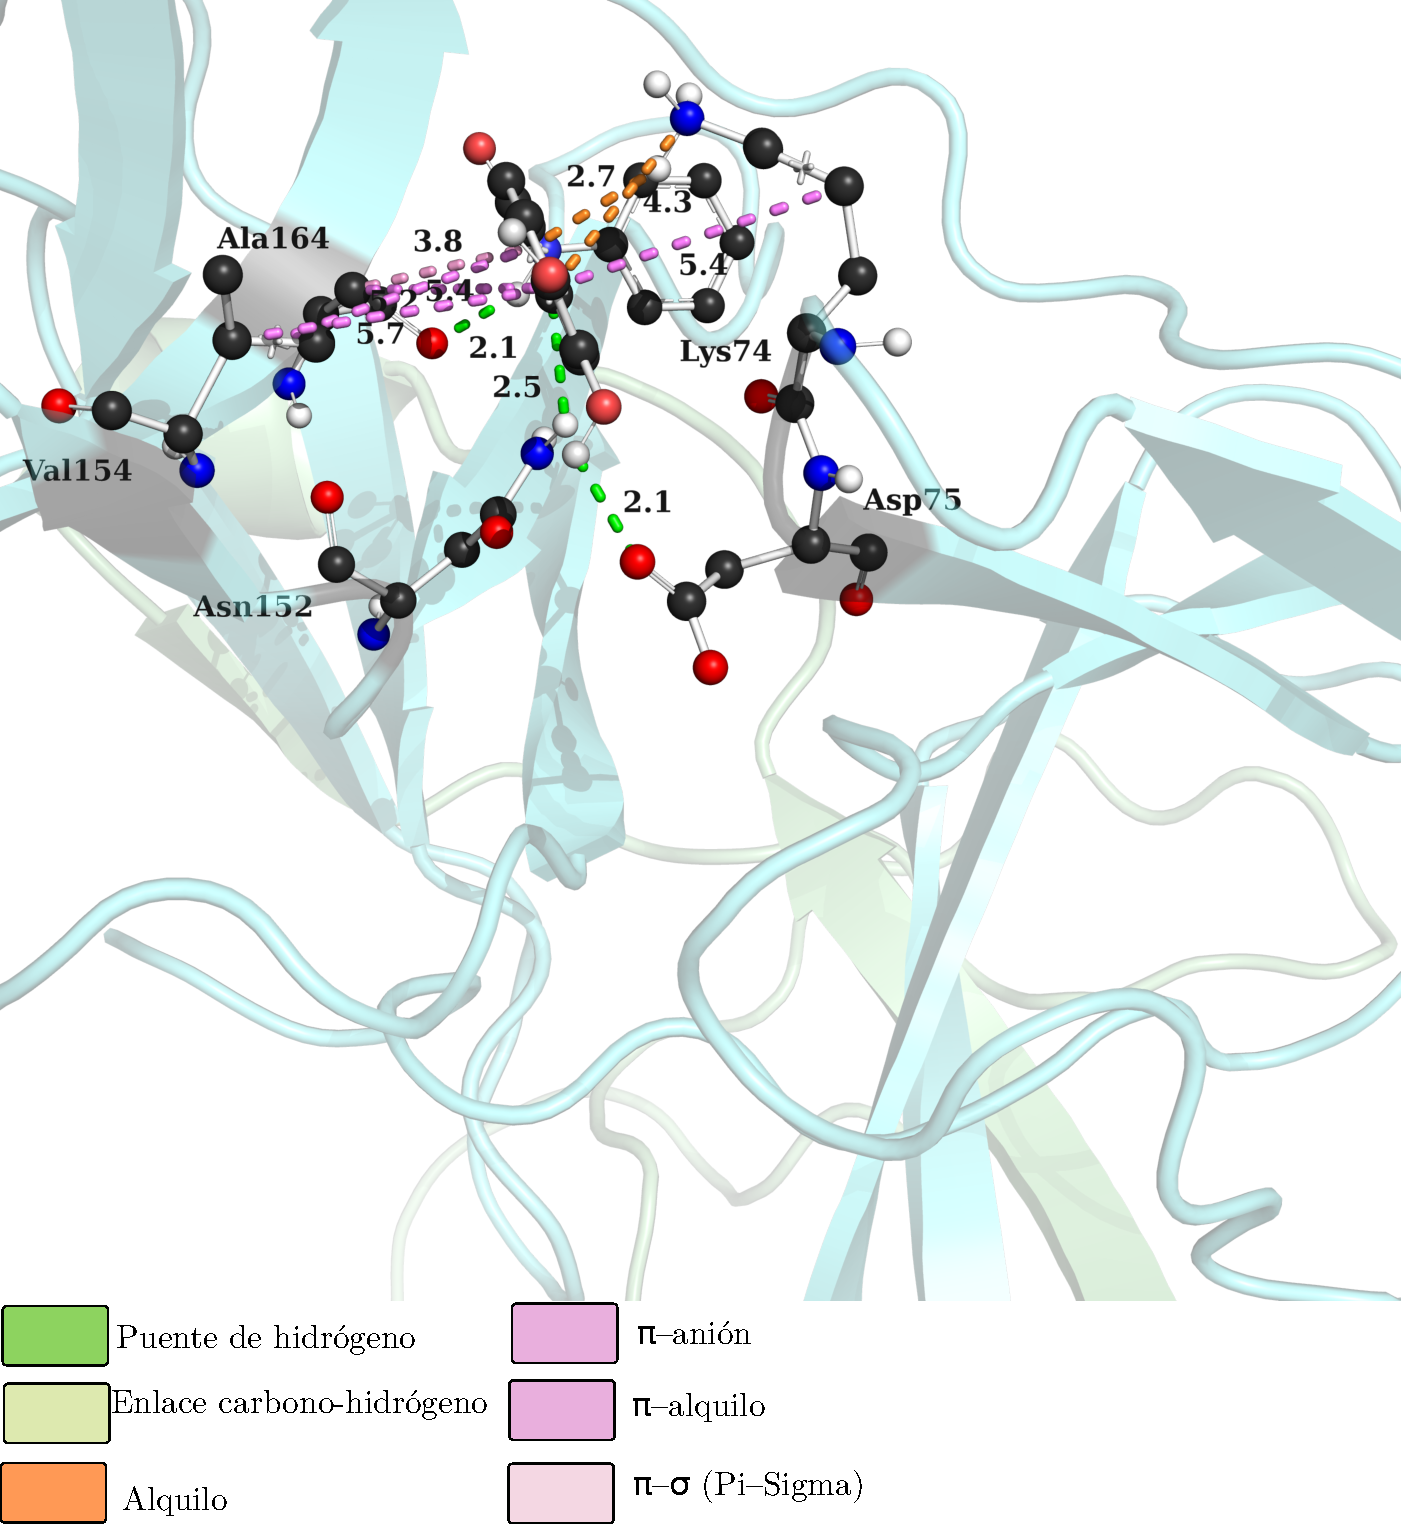
\includegraphics[width=1.0\textwidth]{imagenes/Resu/benza.pdf}
      \caption{Representación del acoplamiento molecular del derivado benzamida en la cavidad alostérica de la proteasa NS2B-NS3.
      Se presentan las distancias de enlace expresadas en (\AA).}
      \label{fig:benzamida-3d}
        \end{figure}

\begin{figure}[H]
      \centering
      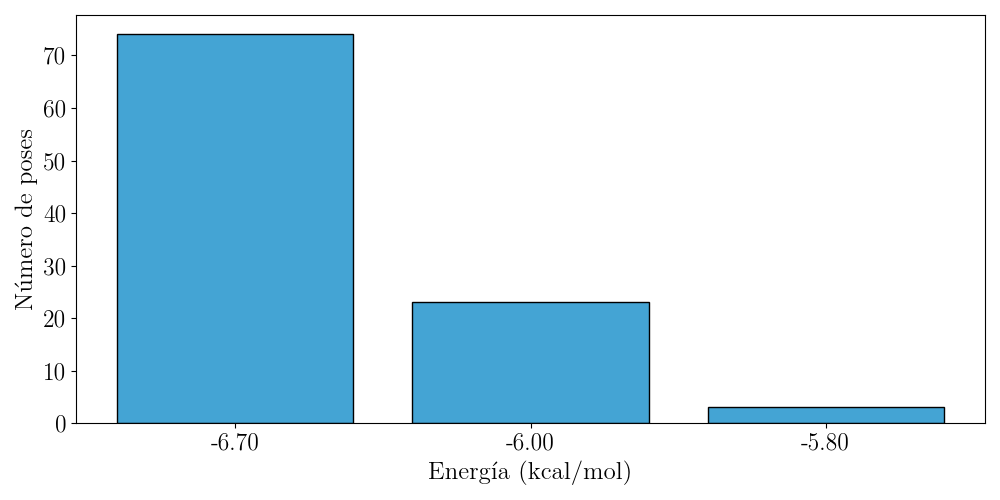
\includegraphics[width=1.0\textwidth]{imagenes/Resu/benza-3.png}
      \caption{Diagrama de contactos del derivado de benzamida con la proteasa NS2B-NS3.}
      \label{fig:benzamida-contactos}
        \end{figure}
        
 \begin{table}[H]
    \centering
    \footnotesize % Tamaño de letra más pequeño para que entre holgadamente
    \setlength{\tabcolsep}{5pt} % Otorga espacio entre columnas para que no se peguen
    \renewcommand{\arraystretch}{1.2}
    \caption{Interacciones no covalentes y distancias de contacto para el acoplamiento del inhibidor alostérico derivado de benzamida en la proteasa de DENV-2.}
    \label{tab:interacciones-2fom}
    \begin{tabular}{llcll}
        \toprule
        \multicolumn{1}{c}{\textbf{\shortstack[c]{Tipo de\\interacción}}} & 
        \multicolumn{1}{c}{\textbf{Residuo}} & 
        \multicolumn{1}{c}{\textbf{\shortstack[c]{Distancia\\(\AA)}}} & 
        \multicolumn{1}{c}{\textbf{\shortstack[c]{Motivo\\estructural}}} & 
        \multicolumn{1}{c}{\textbf{\shortstack[c]{Tipo de\\aminoácido}}} \\
        \midrule
        Puente de hidrógeno & Ala164 & 2.07 & Sitio de unión & Apolar / Hidrofóbico \\
                            & Asn152 & 2.52 & Sitio de unión & Polar no cargado \\
                            & Asp75  & 2.12 & Tríada catalítica & Polar, cargado negativo \\
        \midrule
        $\pi$-Catión        & Lys74  & 2.62 & Bolsillo S1 / Sitio activo & Polar, cargado positivo \\
                            & Lys74  & 4.27 & Bolsillo S1 / Sitio activo & Polar, cargado positivo \\
        \midrule
        Interacción hidrofóbica & Val154 & 4.91 & Bolsillo hidrofóbico & Apolar / Hidrofóbico \\
                                & Val154 & 5.16 & Bolsillo hidrofóbico & Apolar / Hidrofóbico \\
                                & Val154 & 5.40 & Bolsillo hidrofóbico & Apolar / Hidrofóbico \\
        \bottomrule
    \end{tabular}
\end{table}
      Se seleccionó la conformación de menor energía ($-6.00 \text{ kcal/mol}$) por presentar el anclaje mediante puente de hidrógeno con el residuo Gly133 del hueco oxianiónico, permitiendo evaluar mediante dinámica molecular la estabilidad temporal de esta interacción. 

Con un límite de 5.0 y una exhaustividad de 80, se obtuvieron tres grupos: 74 modelos con -6.70 kcal/mol, 3 modelos con -5.80 kcal/mol y 23 modelos con -6.00 kcal/mol. 

Como se observa en el perfil energético de la Figura~\ref{fig:benzamida-contactos}, el acoplamiento molecular exhibió una marcada convergencia conformacional. La conformación de menor energía libre de unión alcanzó un valor de $-6.70\ \text{kcal/mol}$, concentrando un 74\% del total de las poses generadas. Esta distribución sugiere que el modo de unión es una pose termodinámicamente favorable en el bolsillo alostérico.
Al contrastar los contactos atómicos obtenidos (Tabla~\ref{tab:potencial-electrostatico} y Figura~\ref{fig:benzamida-3d}) con los hallazgos reportados en la literatura para inhibidores alostéricos de estructura similar (como el derivado de benzofurano 34e, $\text{IC}_{50} = 0.69\ \mu\text{M}$), se identifican importantes coincidencias estructurales y mecanísticas:

\begin{itemize}
    \item \textbf{Red de puentes de hidrógeno y el ``interruptor molecular'' (\textbf{Asn152}):} En nuestros resultados, el oxígeno del anillo de benzofurano establece un puente de hidrógeno convencional con la cadena lateral de \textbf{Asn152} a una distancia de $2.52\ \text{\AA}$. Este hallazgo es de vital relevancia, ya que la literatura señala a \textbf{Asn152} como un ``interruptor molecular'' clave responsable de mantener a la enzima en su conformación inactiva. Adicionalmente, el grupo hidroxilo del anillo aromático forma un puente de hidrógeno fuerte de $2.12\ \text{\AA}$ con \textbf{Asp75} (perteneciente a la tríada catalítica), mientras que el grupo N--H de la amida interactúa mediante un enlace de hidrógeno de $2.07\ \text{\AA}$ con el esqueleto de \textbf{Ala164}. Esta red tripartita de puentes de hidrógeno ancla firmemente el ligando al sitio de unión.
    
    \item \textbf{Interacciones electrostáticas y $\pi$-catiónicas con \textbf{Lys74}:} La literatura reporta que en derivados como el 34e, la orientación inclinada del núcleo aromático y el carbonilo amídico permite una interacción crítica con \textbf{Lys74}. En nuestros cálculos de \textit{docking}, se confirmó la participación activa de este residuo mediante dos interacciones de tipo $\pi$-catión con el sistema aromático del compuesto a distancias de $2.62\ \text{\AA}$ y $4.27\ \text{\AA}$. Esta atracción electrostática refuerza la fijación del andamio en la entrada del bolsillo S1/alostérico.
    
    \item \textbf{Complementariedad en el subbolsillo hidrofóbico:} El análisis de contactos no polares reveló interacciones de tipo $\pi$-sigma y $\pi$-alquil entre el sistema aromático y el residuo \textbf{Val154} ($4.91\ \text{\AA}$, $5.16\ \text{\AA}$ y $5.40\ \text{\AA}$). Aunque los estudios reportados previamente destacan la inserción lipofílica hacia residuos como \textbf{Leu76}, \textbf{Gly148} e \textbf{Ile165}, el contacto hallado con \textbf{Val154} demuestra una acomodación hidrofóbica equivalente que estabiliza el núcleo aromático dentro de la cavidad no polar.
\end{itemize}

Los datos \textit{in silico} obtenidos respaldan el mecanismo de inhibición alostérica no competitiva previamente sustentado por estudios cinéticos  y de mutagénesis dirigida (T122C). Al alojarse en la cavidad posterior cerca del residuo \textbf{Thr122} e interactuar directamente con la tríada catalítica (\textbf{Asp75}) y los residuos de control conformacional (\textbf{Asn152} y \textbf{Lys74}), el ligando bloquea la flexibilidad funcional requerida para el procesamiento del sustrato poliproteico.

En conjunto, la consistencia entre los valores de energía observados, la baja distancia de los puentes de hidrógeno ($\le 2.52\ \text{\AA}$) y la concordancia con los residuos clave descritos en la literatura confirman la efectividad del núcleo molecular evaluado como un candidato prometedor para el desarrollo de fármacos antivirales selectivos contra DENV-2.
 
 \begin{figure}[H]
      \centering
      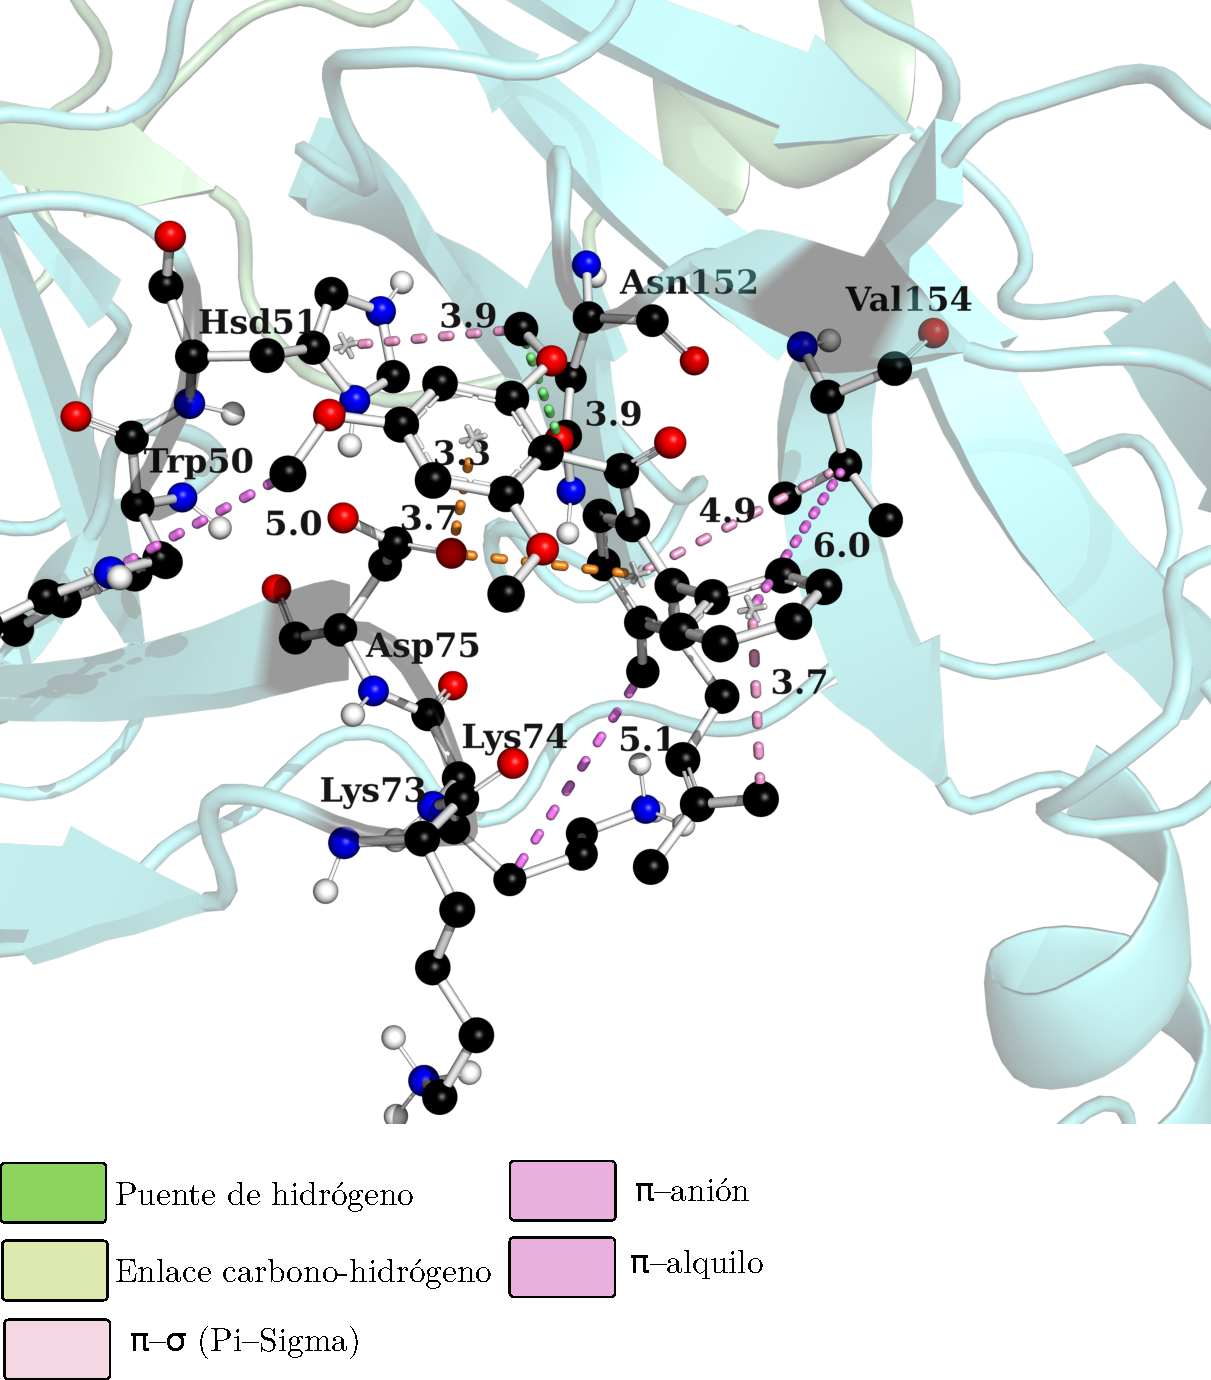
\includegraphics[width=1.0\textwidth]{imagenes/Resu/246.pdf}
      \caption{Representación del acoplamiento molecular del derivado 246DA en la cavidad ortostérica de la proteasa NS2B-NS3. Se presentan las distancias de enlace expresadas en (\AA).}
      \label{fig:246-3d}
        \end{figure}
       
\begin{figure}[H]
      \centering
      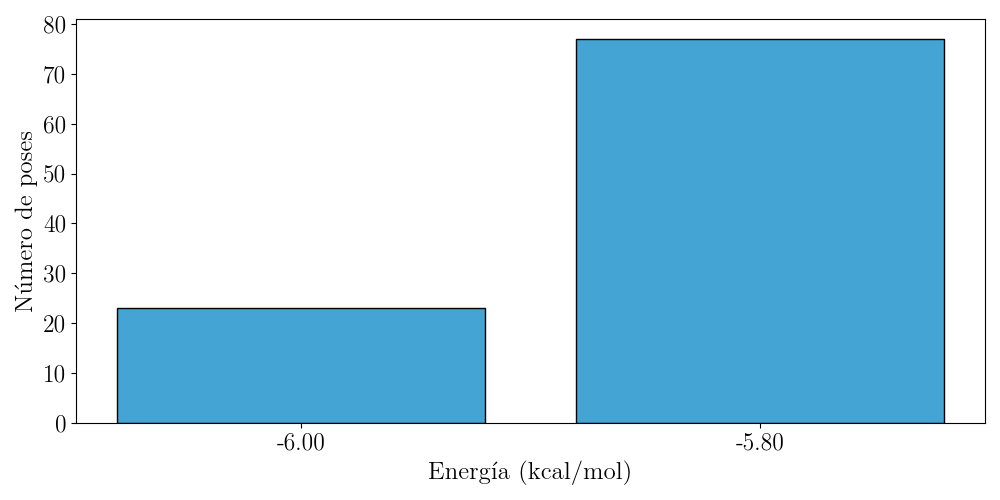
\includegraphics[width=1.0\textwidth]{imagenes/Resu/246-1.png}
      \caption{Diagrama de contactos del compuesto de referencia identificado como 246DA en el archivo de imagen.}
      \label{fig:246-contactos}
        \end{figure}

  \begin{table}[H]
    \centering
    \footnotesize
    \setlength{\tabcolsep}{5pt}
    \renewcommand{\arraystretch}{1.2}
    \caption{Interacciones no covalentes y distancias de contacto para el acoplamiento del inhibidor ortostérico 264DA en la proteína NS2B-NS3.}
    \label{tab:interacciones-pose83}
    \begin{tabular}{llcll}
        \toprule
        \multicolumn{1}{c}{\textbf{\shortstack[c]{Tipo de\\interacción}}} & 
        \multicolumn{1}{c}{\textbf{Residuo}} & 
        \multicolumn{1}{c}{\textbf{\shortstack[c]{Distancia\\(\AA)}}} & 
        \multicolumn{1}{c}{\textbf{\shortstack[c]{Motivo\\estructural}}} & 
        \multicolumn{1}{c}{\textbf{\shortstack[c]{Tipo de\\aminoácido}}} \\
        \midrule
        Enlace de H de carbono & Asn152 & 3.76 & Sitio de unión & Polar no cargado \\
        \midrule
        $\pi$-Anión            & Asp75  & 3.28 & Tríada catalítica & Polar, cargado negativo \\
                               & Asp75  & 3.88 & Tríada catalítica & Polar, cargado negativo \\
        \midrule
        $\pi$-Sigma            & Val154 & 3.07 & Bolsillo hidrofóbico & Apolar / Hidrofóbico \\
                               & Hsd51  & 3.85 & Tríada catalítica & Polar, cargado positivo \\
        \midrule
        Interacción hidrofóbica & Trp50  & 4.03 & Bolsillo hidrofóbico & Apolar / Aromático \\
        (Alquil / $\pi$-Alquil) & Lys74  & 4.42 & Bolsillo S1 / Sitio activo & Polar, cargado positivo \\
                               & Val154 & 4.72 & Bolsillo hidrofóbico & Apolar / Hidrofóbico \\
                               & Val154 & 5.32 & Bolsillo hidrofóbico & Apolar / Hidrofóbico \\
        \bottomrule
    \end{tabular}
\end{table}




El análisis del acoplamiento molecular realizado mediante el programa AutoDock Vina (configurado con una exhaustividad de 80) permitió evaluar la afinidad y el modo de unión del ligando en el sitio catalítico del receptor. A partir de una muestra de 100 poses generadas, el perfil energético reveló la presencia de dos conformaciones principales: un primer grupo de 23 poses con una energía libre de unión de $-6.00\ \text{kcal/mol}$ y un segundo conglomerado (\textit{cluster}) predominante correspondiente a 77 poses con una energía de $-5.80\ \text{kcal/mol}$ (Figura~\ref{fig:246-contactos}).

A pesar de que el primer grupo presentó el valor de energía mínimo absoluto, la selección final del modo de acoplamiento recayó en una de las conformaciones del ligando ortosterico reportado en la literatura como 246DA (perteneciente al \textit{cluster} de $-5.80\ \text{kcal/mol}$). Esta decisión se fundamenta en un criterio estadístico y termodinámico: la representación poblacional del 77\% sugiere una mayor probabilidad de ocurrencia del estado conformacional en equilibrio. Además, la diferencia energética de apenas $\Delta E = 0.2\ \text{kcal/mol}$ entre ambos mínimos se encuentra bien dentro del margen del ruido térmico (a temperatura ambiente), lo que demuestra que ambas poses son energéticamente equivalentes pero la conformación ganadora del inhibidor  es representativa de la microconformación más probable.

La inspección visual y la caracterización de los contactos no covalentes  (Tabla~\ref{tab:interacciones-pose83} y Figura~\ref{fig:246-3d}) permitieron identificar el patrón de interacciones que estabiliza dicho complejo:

\begin{itemize}
    \item \textbf{Enlaces de Carbono-Hidrógeno y contactos polares:} Se observaron interacciones fuertemente estabilizadoras mediadas por enlaces de carbono-hidrógeno, destacando el papel del residuo polar no cargado \textbf{Asn152}. Este residuo actúa como un ancla clave en la cavidad al interaccionar directamente con los átomos de carbono-hidrógeno del ligando a distancias cortas de contacto.
    \item \textbf{Interacciones electrostáticas y relativas a electrones $\pi$:} Se identificaron interacciones del tipo $\pi$-anión y $\pi$-sigma con los residuos de la tríada catalítica y del contorno del sitio activo (\textbf{His51}, \textbf{Asp75} y \textbf{Lys74}), así como contactos hidrofóbicos ($\pi$-alquilo / alquilo) con residuos como \textbf{Val154} y \textbf{Trp50}.
\end{itemize}

Al contrastar nuestros resultados con el estudio de referencia reportado por literatura para el inhibidor sintético 246DA  acoplado en la proteasa NS2B/NS3 del serotipo 2 del virus del dengue, se observa una coincidencia estructural y funcional sobresaliente. En la literatura se reporta que la potencia del compuesto 246DA radica en su capacidad para interaccionar mediante puentes de hidrógeno directos con la tríada catalítica (\textbf{His51}, \textbf{Asp75} y \textbf{Ser135}), a la vez que ocupa el bolsillo hidrofóbico coordinándose con residuos como \textbf{Leu76}, \textbf{Trp83}, \textbf{Ile165} e \textbf{Ile166}. 

Nuestras observaciones reafirman que esta conformación adopta una orientación tridimensional coherente con dicho modelo bioactivo. Aunque nuestro acoplamiento con AutoDock Vina prioriza las fuerzas de van der Waals, electrostáticas y enlaces C--H con residuos como \textbf{Asn152}, \textbf{His51} y \textbf{Asp75}, la conservación del anclaje en los residuos de la tríada catalítica confirma la validez biológica del acoplamiento. Esto sugiere que el complejo obtenido reproduce los requerimientos farmacofóricos necesarios para la inhibición competitiva de la proteasa viral DENV2.
    
\begin{figure}[H]
      \centering
      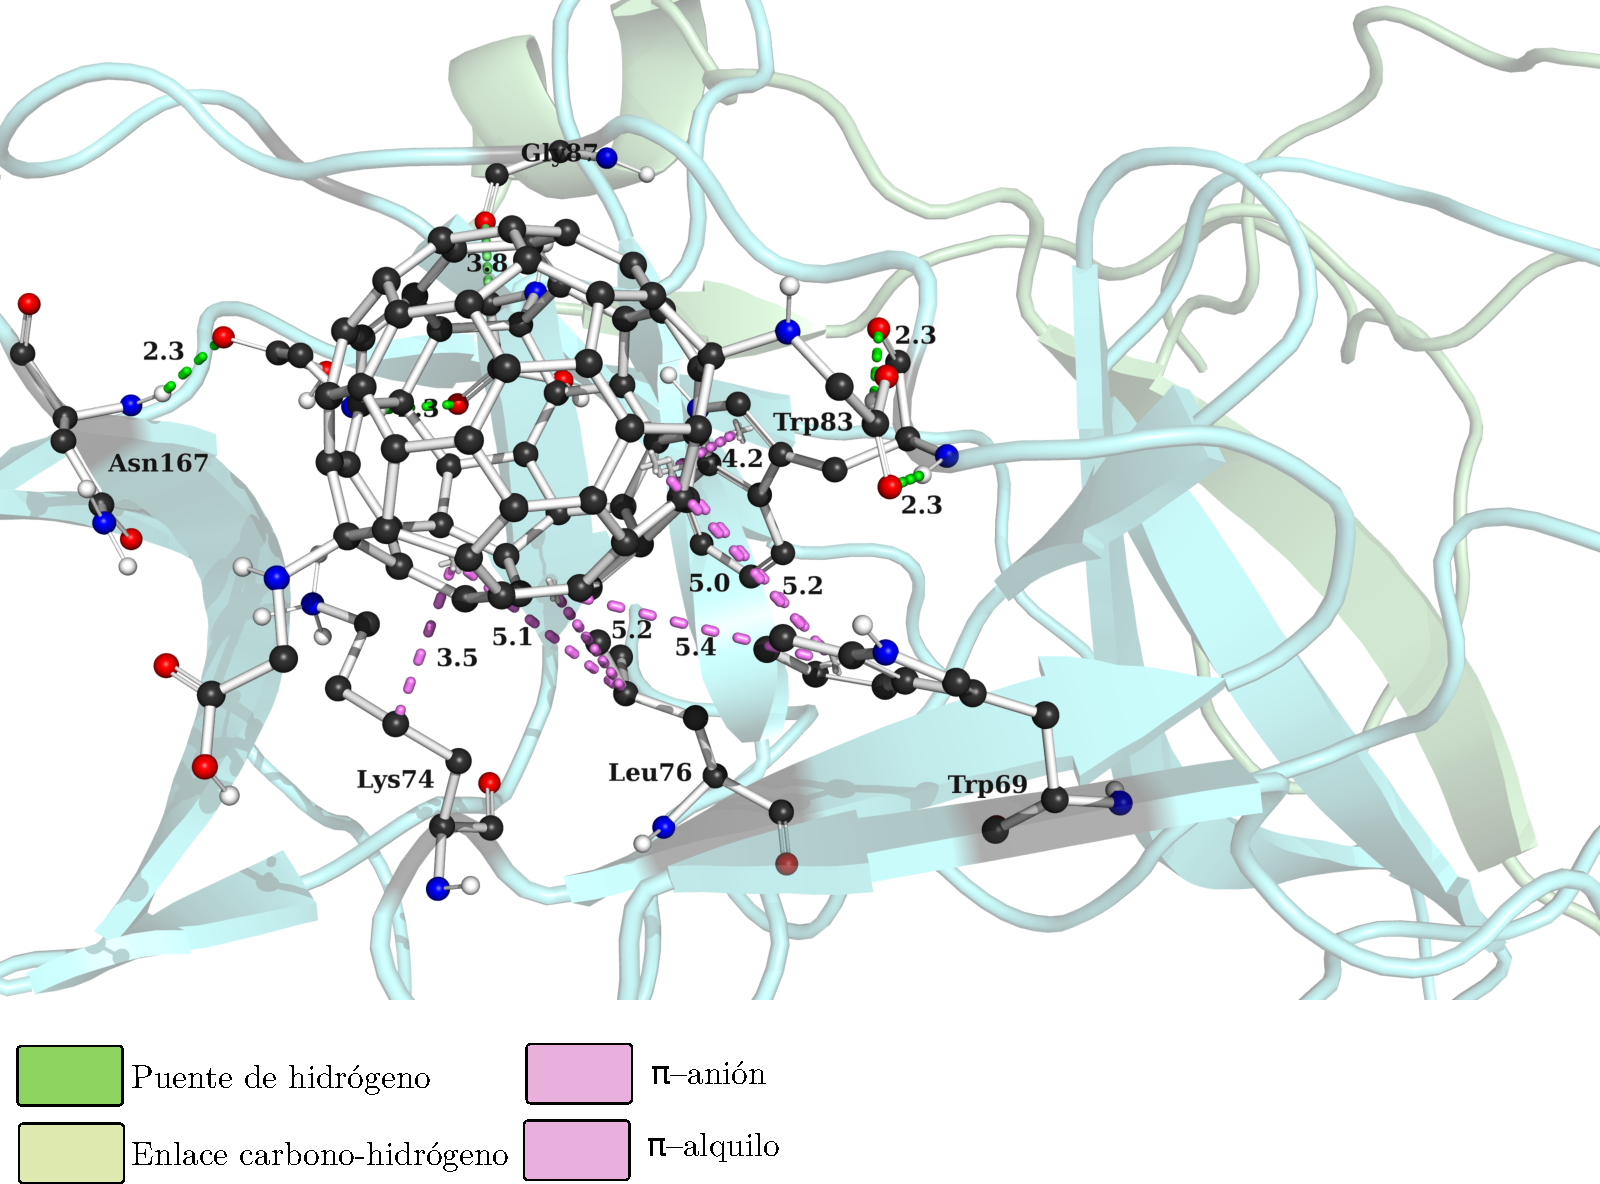
\includegraphics[width=1.0\textwidth]{imagenes/Resu/ciego.pdf}
      \caption{Resultados gráficos del acoplamiento ciego del aducto de fullereno con glicina.}
      \label{fig:ciego-perfil}
        \end{figure}
        
\begin{figure}[H]
      \centering
      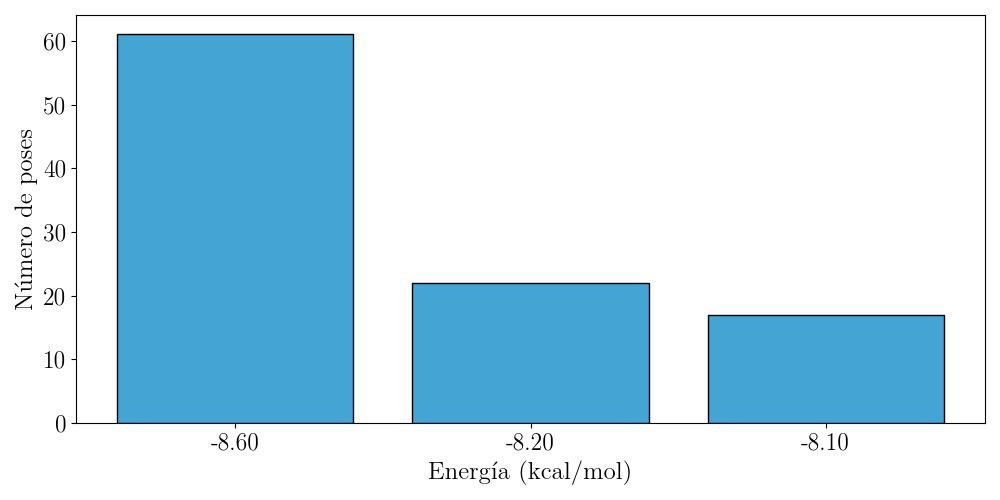
\includegraphics[width=1.0\textwidth]{imagenes/Resu/ciego.png}
      \caption{Diagrama de contactos del acoplamiento ciego del aducto dC\textsubscript{60}(Gly)\textsubscript{4}.}
      \label{fig:ciego-contactos}
        \end{figure}
        
   \begin{table}[H]
    \centering
    \footnotesize
    \setlength{\tabcolsep}{5pt}
    \renewcommand{\arraystretch}{1.2}
    \caption{Interacciones no covalentes y distancias de contacto para el acoplamiento ciego del derivado de fulereno C\textsubscript{60}(Gly)\textsubscript{4} en la proteasa NS2B-NS3.}
    \label{tab:interacciones-pose72}
    \begin{tabular}{llcll}
        \toprule
        \multicolumn{1}{c}{\textbf{\shortstack[c]{Tipo de\\interacción}}} & 
        \multicolumn{1}{c}{\textbf{Residuo}} & 
        \multicolumn{1}{c}{\textbf{\shortstack[c]{Distancia\\(\AA)}}} & 
        \multicolumn{1}{c}{\textbf{\shortstack[c]{Motivo\\estructural}}} & 
        \multicolumn{1}{c}{\textbf{\shortstack[c]{Tipo de\\aminoácido}}} \\
        \midrule
        Puente de hidrógeno & Lys74  & 2.92 & Bolsillo S1 / Sitio activo & Polar, cargado positivo \\
        \midrule
        Enlace de H de carbono & Asp174 & 3.26 & Sitio de unión & Polar, cargado negativo \\
                            & Asn167 & 3.40 & Sitio de unión & Polar no cargado \\
                            & Gly48 & 3.78 & Sitio de unión & Apolar / Neutro \\
        \midrule
        Interacción hidrofóbica & Trp83  & 5.24 & Bolsillo hidrofóbico & Apolar / Aromático \\
        ($\pi$-Alquil) & & & & \\
        \bottomrule
    \end{tabular}
\end{table}
     El análisis del acoplamiento ciego realizado mediante el programa AutoDock Vina permitió evaluar la capacidad de interacción, la afinidad termodinámica y el modo de unión del derivado de fulereno tetraaducto de glicina (C\textsubscript{60}(Gly)\textsubscript{4}) sobre la estructura tridimensional de la proteasa NS2B/NS3 del serotipo 2 del virus del dengue. A partir de un muestreo de 100 poses generadas, el perfil energético reveló una distribución conformacional dividida en tres conglomerados (\textit{clusters}) principales: un primer grupo mayoritario de 61 poses con una energía libre de unión de $-8.60\ \text{kcal/mol}$, seguido de un segundo grupo de 22 poses con $-8.20\ \text{kcal/mol}$ y un tercer grupo de 17 poses con $-8.10\ \text{kcal/mol}$ (Figura~\ref{fig:ciego-contactos}).

La selección del modo de acoplamiento óptimo del C\textsubscript{60}(Gly)\textsubscript{4} recayó en el \textit{cluster} perteneciente al mínimo energético absoluto de $-8.60\ \text{kcal/mol}$. A diferencia de sistemas donde el mínimo energético y la densidad conformacional divergen, en este caso coinciden ambos criterios: la amplia representación poblacional (61\%) demuestra que esta conformación no solo es la más estable termodinómicamente, sino también  en equilibrio más probable durante el proceso de reconocimiento molecular. Asimismo, el valor atrayente de $-8.60\ \text{kcal/mol}$ refleja una afinidad sustancialmente elevada, favorecida por la naturaleza anfifílica del aducto, el cual combina el núcleo hidrofóbico del fulereno C\textsubscript{60} con las cadenas polares de glicina.

La caracterización detallada de los contactos no covalentes efectuada mediante PyMOL y Discovery Studio Visualizer (Tabla~\ref{tab:interacciones-pose72} y Figura~\ref{fig:ciego-perfil}) permitió dilucidar el patrón de interacciones responsables de la estabilización del complejo nanoestructura-proteína:

\begin{itemize}
    \item \textbf{Puentes de hidrógeno convencionales:} Se identificó un puente de hidrógeno fuerte entre el grupo carboxilo/amino de las cadenas de glicina del ligando y el residuo \textbf{Lys74} a una distancia de $2.92\ \text{\AA}$. Este contacto en el subsitio S1 / entorno del sitio activo actúa como un ancla electrostática y polar determinante para la orientación del aducto.
    \item \textbf{Enlaces de hidrógeno no convencionales (C--H):} Se detectaron interacciones estabilizadoras débiles tipo $\text{C--H}\cdots\text{O/N}$ con los residuos \textbf{Asp174} ($3.26\ \text{\AA}$), \textbf{Asn167} ($3.40\ \text{\AA}$) y \textbf{Gly48} ($3.78\ \text{\AA}$), las cuales contribuyen a fijar los sustituyentes de glicina a lo largo del contorno de la cavidad de unión.
    \item \textbf{Interacciones hidrofóbicas ($\pi$-Alquil):} El núcleo aromático de la esfera de fulereno establece contactos lipofílicos de tipo $\pi$-alquilo con el residuo aromático \textbf{Trp83} a una distancia de $5.24\ \text{\AA}$, acomodándose adecuadamente dentro del bolsillo hidrofóbico de la proteasa.
\end{itemize}

Al contrastar estos resultados con la literatura reportada para aductos de fulereno-glicina (C\textsubscript{60}(Gly)), se constata una consistencia notable con las propiedades fisicoquímicas y de unión a proteínas descritas experimentalmente. En estudios previos se ha demostrado mediante calorimetría de titulación isotérmica (ITC) que los aductos de C\textsubscript{60}(Gly) presentan una elevada constante de asociación con proteínas séricas humanas, impulsada principalmente por fuerzas hidrofóbicas y solvatación favorable, sin generar efectos citotóxicos ni genotóxicos significativos. De manera análoga, nuestros resultados \textit{in silico} confirman que el C\textsubscript{60}(Gly)\textsubscript{4} posee la versatilidad estructural para insertarse en la cavidad catalítica de la proteasa DENV2, acoplándose simultáneamente al subsitio S1 (\textbf{Lys74}) y al bolsillo hidrofóbico (\textbf{Trp83}).

En conjunto, la conservación de estos anclajes clave y la alta afinidad calculada sugerirían que el acoplamiento ciego logra ocluir estéricamente el sitio activo de la proteasa NS2B/NS3, validando la hipótesis de que el derivado C\textsubscript{60}(Gly)\textsubscript{4} se comporta como un potencial inhibidor competitivo o nano-plataforma bioactiva contra el virus del dengue serotipo 2.
        
\begin{figure}[H]
      \centering
      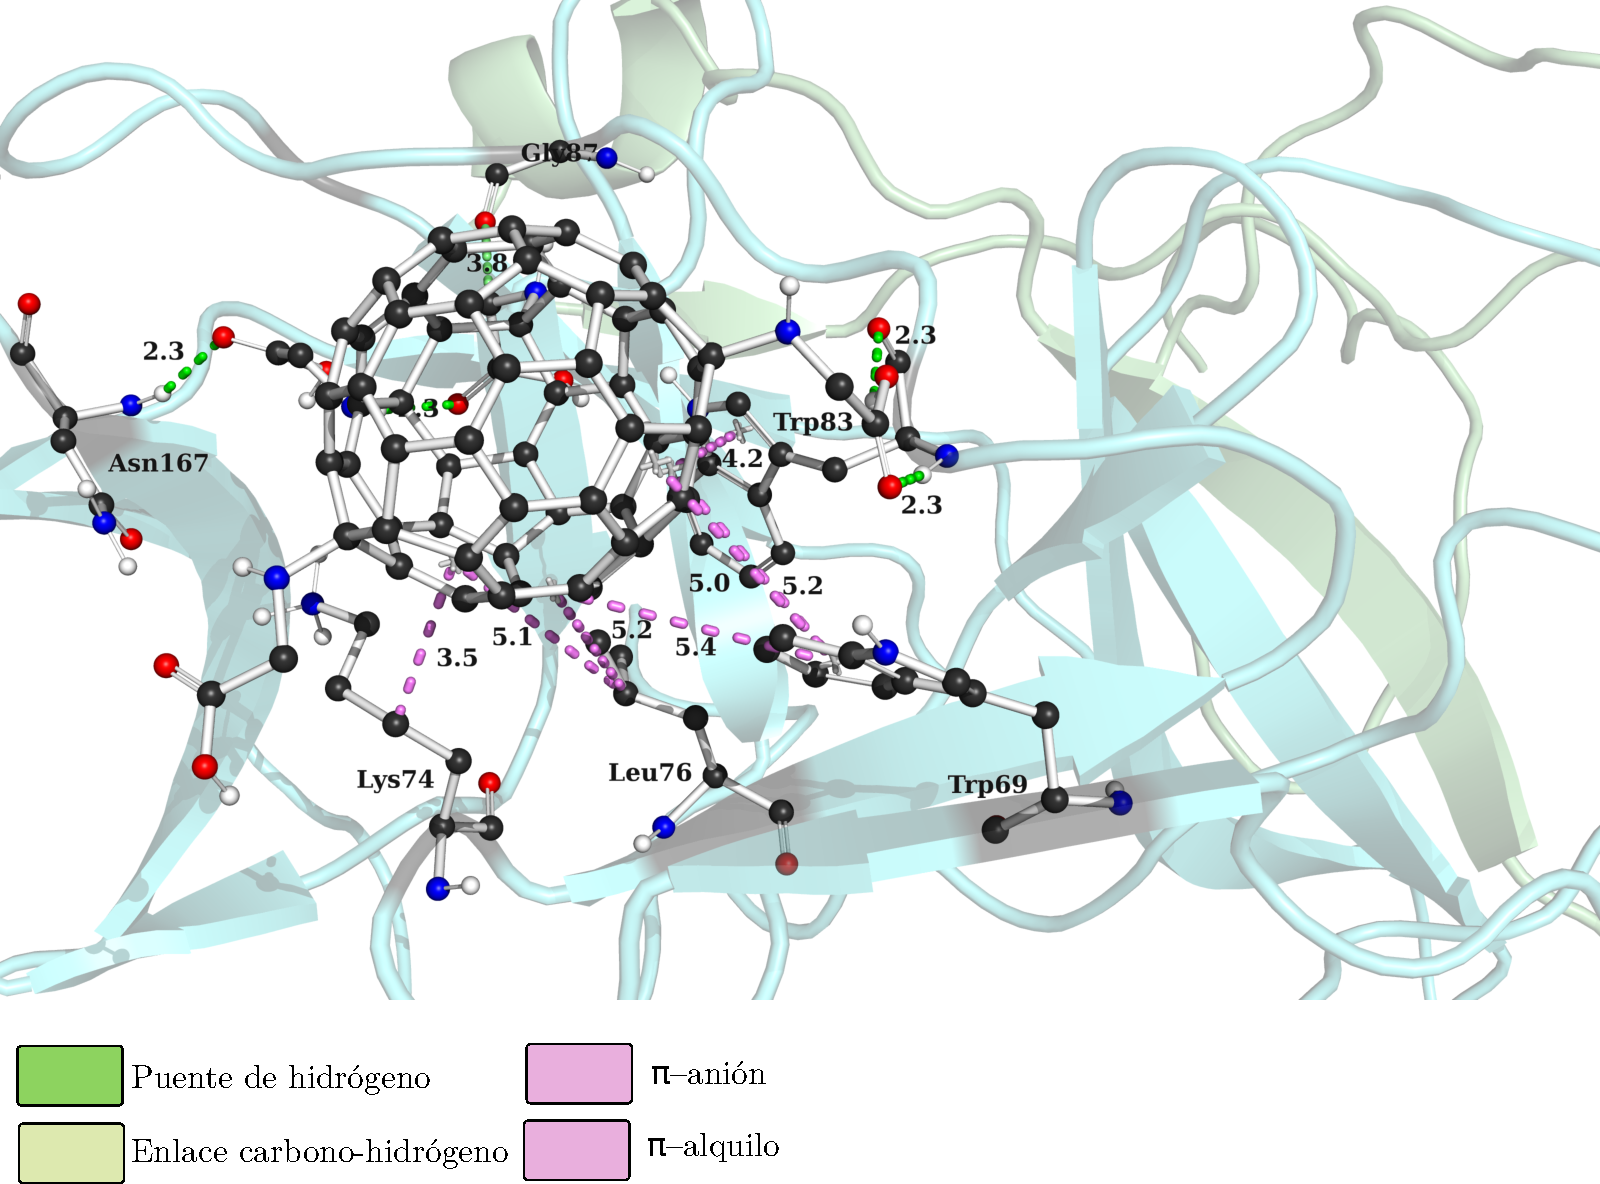
\includegraphics[width=1.0\textwidth]{imagenes/Resu/repor-c60.pdf}
      \caption{Resultados gráficos del acoplamiento dirigido del C\textsubscript{60}(Gly)\textsubscript{4} a la región alostérica.}
      \label{fig:alosterico-perfil}
        \end{figure}

\begin{figure}[H]
      \centering
      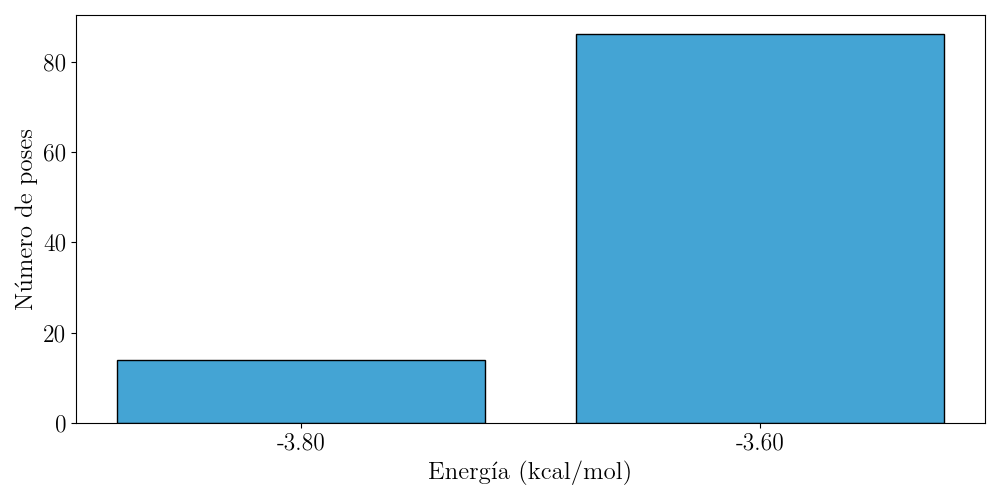
\includegraphics[width=1.0\textwidth]{imagenes/Resu/alo-resu-c60.png}
      \caption{Diagrama de contactos del aducto en la región alostérica.}
      \label{fig:alosterico-contactos}
        \end{figure}
        
 \begin{table}[H]
    \centering
    \footnotesize
    \setlength{\tabcolsep}{5pt}
    \renewcommand{\arraystretch}{1.2}
    \caption{Interacciones no covalentes y distancias de contacto para el acoplamiento del derivado de fulereno C\textsubscript{60}(Gly)\textsubscript{4} en la proteasa NS2B-NS3.}
    \label{tab:interacciones-pose61}
    \begin{tabular}{llcll}
        \toprule
        \multicolumn{1}{c}{\textbf{\shortstack[c]{Tipo de\\interacción}}} & 
        \multicolumn{1}{c}{\textbf{Residuo}} & 
        \multicolumn{1}{c}{\textbf{\shortstack[c]{Distancia\\(\AA)}}} & 
        \multicolumn{1}{c}{\textbf{\shortstack[c]{Motivo\\estructural}}} & 
        \multicolumn{1}{c}{\textbf{\shortstack[c]{Tipo de\\aminoácido}}} \\
        \midrule
        Puente de hidrógeno & Asn167 & 2.34 & Sitio de unión & Polar no cargado \\
                            & Trp83  & 2.32 & Bolsillo hidrofóbico & Apolar / Aromático \\
        \midrule
        Enlace de H de carbono & Gly87  & 3.67 & Sitio de unión & Apolar / Neutro \\
        \midrule
        Interacción hidrofóbica & Leu76  & 4.78 & Bolsillo hidrofóbico & Apolar / Hidrofóbico \\
        (Alquil / $\pi$-Alquil) & Trp69  & 5.22 & Bolsillo hidrofóbico & Apolar / Aromático \\
                                & Lys74  & 6.12 & Bolsillo S1 / Sitio activo & Polar, cargado positivo \\
        \bottomrule
    \end{tabular}
\end{table}       
\subsection{Evaluación del acoplamiento alostérico del derivado C\textsubscript{60}(Gly)\textsubscript{4}}

El análisis del acoplamiento molecular dirigido hacia el bolsillo alostérico de la proteasa NS2B/NS3 se llevó a cabo bajo los mismos parámetros de exhaustividad 80 para evaluar la capacidad del aducto C\textsubscript{60}(Gly)\textsubscript{4} de actuar como un inhibidor alostérico en el sitio reportado para moléculas pequeñas como las benzamidas. A partir del muestreo de 100 poses generadas, el perfil energético Figura~\ref{fig:alosterico-perfil} mostró una distribución conformacional altamente homogénea pero con valores de afinidad moderados: un grupo de 14 poses con una energía libre de unión de $-3.80\ \text{kcal/mol}$ y un conglomerado predominantemente mayoritario correspondiente a 86 poses con una energía de $-3.60\ \text{kcal/mol}$.

La selección del modo de acoplamiento al sitio alostérico reportado recayó en el \textit{cluster} perteneciente al grupo de mínima energía de $-3.80\ \text{kcal/mol}$. La diferencia energética entre ambos mínimos ($\Delta G = 0.20\ \text{kcal/mol}$) se encuentra holgadamente contenida dentro del margen del ruido térmico ($k_B T \approx 0.60\ \text{kcal/mol}$ a temperatura ambiente, lo que demuestra que ambas poblaciones representan microconformaciones equivalentes en rápido equilibrio termodinámico a lo largo de la entrada de la cavidad alostérica.

La caracterización visual y atómica de las interacciones no covalentes Tabla~\ref{tab:interacciones-pose61} y Figura~\ref{fig:alosterico-perfil}) permitió identificar el patrón de estabilización de la:

\begin{itemize}
    \item \textbf{Puentes de hidrógeno convencionales:} Se observaron dos puentes de hidrógeno fuertes mediados por los sustituyentes de glicina del aducto con la cadena lateral de \textbf{Asn167} ($2.34\ \text{\AA}$, polar no cargado) y con el residuo aromático \textbf{Trp83} ($2.32\ \text{\AA}$), fijando las cadenas polares externas en el contorno del sitio alostérico.
    \item \textbf{Enlaces de hidrógeno de carbono (C--H):} Se identificó un contacto débil tipo $\text{C--H}\cdots\text{O/N}$ entre el esqueleto del ligando y el residuo \textbf{Gly87} a una distancia de $3.67\ \text{\AA}$.
    \item \textbf{Interacciones hidrofóbicas (Alquil / $\pi$-Alquil):} La esfera carbonosa del fulereno interacciona mediante contactos lipofílicos con los residuos \textbf{Leu76} ($4.78\ \text{\AA}$) y \textbf{Trp69} ($5.22\ \text{\AA}$) en el subbolsillo hidrofóbico, además de mantener un contacto de tipo alquilo/electrostático extendido con \textbf{Lys74} ($6.12\ \text{\AA}$).
\end{itemize}

\subsection{Análisis comparativo entre el derivado de fulereno y el inhibidor alostérico (benzamida/benzofurano)}
\begin{enumerate}
    \item \textbf{Superioridad energética e incremento de afinidad:}
    El derivado de benzamida presenta una estabilidad y afinidad termodinámica superior al alcanzar una energía libre de unión de $-6.70\text{ kcal/mol}$ (con poses de hasta $-5.80\text{ kcal/mol}$), superando notoriamente la afinidad moderada de $-3.60\text{ kcal/mol}$ (con un límite de $-3.80\text{ kcal/mol}$) registrada por el aducto C\textsubscript{60}(Gly)\textsubscript{4}, lo que evidencia un acoplamiento significativamente menos favorable en la cavidad alostérica por parte del fulereno.

    \item \textbf{Conservación y ampliación del farmacóforo catalítico:}
    Mientras que el derivado de benzamida logra un anclaje directo con el residuo de la tríada catalítica Asp75 mediante un puente de hidrógeno corto ($2.12\text{ \AA}$) e interacciones clave con Ala164 ($2.07\text{ \AA}$), Asn152 ($2.52\text{ \AA}$) y Lys74 ($\pi$-catión a $2.62\text{ \AA}$), el C\textsubscript{60}(Gly)\textsubscript{4} no establece contacto directo con la tríada catalítica, limitando su red de puentes de hidrógeno a interacciones externas mediante sus brazos de glicina con Asn167 ($2.34\text{ \AA}$) y Trp83 ($2.32\text{ \AA}$).

    \item \textbf{Acomodación en el bolsillo lipofílico:}
    Al ser una molécula pequeña y compacta, la benzamida se acomoda profundamente dentro de la cavidad alostérica, logrando un empaquetamiento optimizado con Val154 ($4.91\text{ -- }5.40\text{ \AA}$). En contraste, el núcleo esférico y voluminoso del C\textsubscript{60}(Gly)\textsubscript{4} le impide penetrar al fondo del bolsillo, manteniéndose en una disposición más periférica donde su estabilidad depende de interacciones hidrofóbicas dispersas ($\pi$-alquilo) con Leu76 ($4.78\text{ \AA}$), Trp69 ($5.22\text{ \AA}$) y Lys74 ($6.12\text{ \AA}$).
\end{enumerate}


\begin{figure}[H]
      \centering
      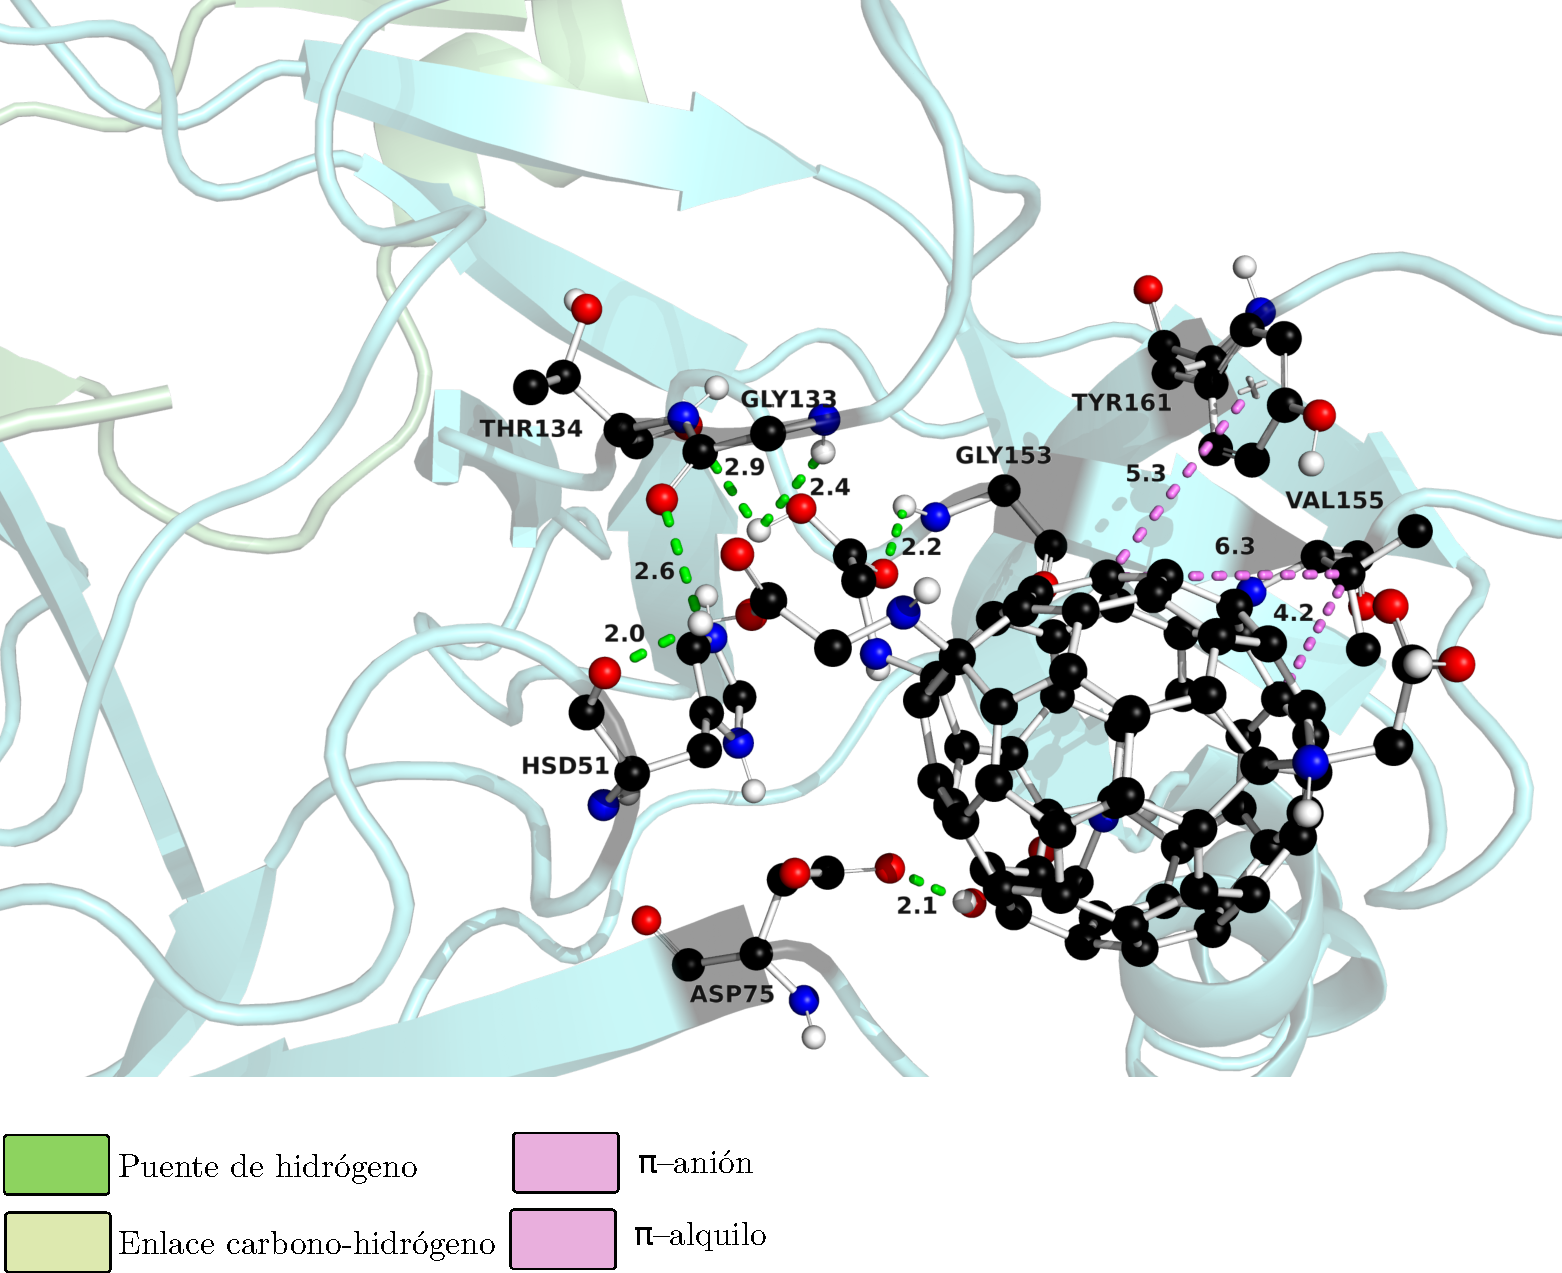
\includegraphics[width=1.0\textwidth]{imagenes/Resu/orto-1.pdf}
      \caption{Resultados gráficos del acoplamiento dirigido a la región ortostérica del  C\textsubscript{60}(Gly)\textsubscript{4}.}
      \label{fig:ortosterico-perfil-2}
        \end{figure}

\begin{figure}[H]
      \centering
      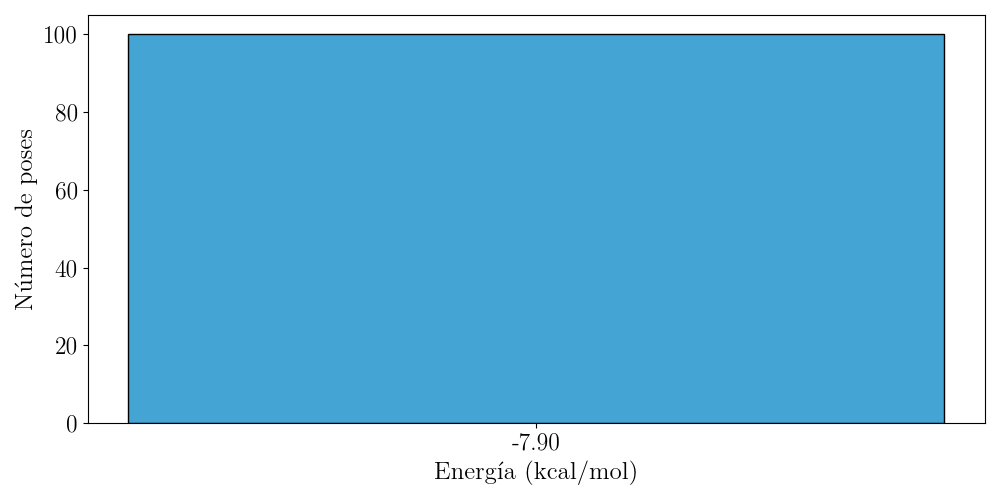
\includegraphics[width=1.0\textwidth]{imagenes/Resu/orto-c60.png}
      \caption{Diagrama de contactos del aducto en la región ortostérica.}
      \label{fig:ortosterico-contactos}
        \end{figure}


\begin{table}[H]
    \centering
    \footnotesize
    \setlength{\tabcolsep}{5pt}
    \renewcommand{\arraystretch}{1.2}
    \caption{Interacciones no covalentes y distancias de contacto para el acoplamiento del derivado de fulereno C\textsubscript{60}(Gly)\textsubscript{4} ortostérico en la proteasa NS2B-NS3.}
    \label{tab:interacciones-pose1}
    \begin{tabular}{llcll}
        \toprule
        \multicolumn{1}{c}{\textbf{\shortstack[c]{Tipo de\\interacción}}} & 
        \multicolumn{1}{c}{\textbf{Residuo}} & 
        \multicolumn{1}{c}{\textbf{\shortstack[c]{Distancia\\(\AA)}}} & 
        \multicolumn{1}{c}{\textbf{\shortstack[c]{Motivo\\estructural}}} & 
        \multicolumn{1}{c}{\textbf{\shortstack[c]{Tipo de\\aminoácido}}} \\
        \midrule
        Puente de hidrógeno & Hsd51  & 2.05 & Tríada catalítica & Polar, cargado positivo \\
                            & Asp75  & 2.83 & Tríada catalítica & Polar, cargado negativo \\
                            & Gly133 & 2.07 & Hueco oxianiónico & Apolar / Neutro \\
                            & Thr134 & 2.63 & Sitio de unión & Polar no cargado \\
                            & Gly153 & 2.15 & Sitio de unión & Apolar / Neutro \\
        \midrule
        Interacción hidrofóbica & Val155 & 4.02 & Bolsillo hidrofóbico & Apolar / Hidrofóbico \\
        (Alquil / $\pi$-Alquil) & Tyr161 & 4.72 & Bolsillo hidrofóbico & Polar neutro / Aromático \\
                                & Tyr161 & 5.24 & Bolsillo hidrofóbico & Polar neutro / Aromático \\
        \bottomrule
    \end{tabular}
\end{table}
El análisis del acoplamiento molecular dirigido al sitio activo ortostérico de la proteasa NS2B/NS3 del serotipo 2 del virus del dengue  demostró una afinidad termodinámica excepcional y un patrón de reconocimiento molecular altamente específico para el aducto C\textsubscript{60}(Gly)\textsubscript{4}. A partir de una muestra de 100 poses generadas mediante AutoDock Vina exhaustividad de 80, el perfil energético Figura~\ref{fig:ortosterico-contactos} exhibió un comportamiento conformacional extraordinario: el 100\% de las poses generadas convergieron en un único conglomerado energéticamente homogéneo con una energía libre de unión  de $-7.90\ \text{kcal/mol}$.

Esta convergencia poblacional del 100\% representa un pozo de energía potencial único y profundamente estable dentro del sitio catalítico, eliminando cualquier ambigüedad conformacional. La selección del modo de unión óptimo recayó en un único \textit{cluster}, el cual ejemplifica el estado en equilibrio dominante y termodinómicamente favorecido en la cavidad ortostérica.


La caracterización tridimensional de las interacciones no covalentes efectuada en PyMOL y Discovery Studio Visualizer (Tabla~\ref{tab:interacciones-pose1} y Figura~\ref{fig:ortosterico-perfil-2}) permitió dilucidar la red de contactos que estabilizan el complejo nanoestructura-proteína:

\begin{itemize}
    \item \textbf{Puentes de hidrógeno convencionales y anclaje catalítico:} Se identificó una densa red de puentes de hidrógeno de corta distancia ($\le 2.83\ \text{\AA}$) coordinados por las cadenas laterales del tetraaducto de glicina:
    \begin{itemize}
        \item Interacción directa con los residuos de la tríada catalítica \textbf{Hsd51} ($2.05\ \text{\AA}$) y \textbf{Asp75} ($2.83\ \text{\AA}$), bloqueando los centros nucleofílico y de transferencia protónica de la enzima.
        \item Formación de un puente de hidrógeno fuerte con el residuo \textbf{Gly133} ($2.07\ \text{\AA}$), perteneciente al \textit{hueco oxianiónico}, un elemento estructural crítico involucrado en la estabilización del estado de transición durante la catálisis peptídica.
        \item Contactos polares adicionales con \textbf{Gly153} ($2.15\ \text{\AA}$) y \textbf{Thr134} ($2.63\ \text{\AA}$), reforzando el posicionamiento del ligando en el contorno del sitio activo.
    \end{itemize}
    
    \item \textbf{Interacciones hidrofóbicas en el bolsillo ortostérico ($\text{Alquil} / \pi\text{-Alquil}$):} La esfera de fulereno se acomoda holgadamente en la cavidad apolar mediante interacciones de tipo $\pi$-alquilo con el residuo hidrofóbico \textbf{Val155} ($4.02\ \text{\AA}$) y contactos aromáticos dobles con la cadena lateral de \textbf{Tyr161} a distancias de $4.72\ \text{\AA}$ y $5.24\ \text{\AA}$.
\end{itemize}

\subsection{Contraste comparativo con el inhibidor reportado 246DA}

Al comparar el desempeño del C\textsubscript{60}(Gly)\textsubscript{4} en este sitio ortostérico con el inhibidor sintético de referencia reportado en la literatura, el compuesto 246DA, se identifican ventajas estructurales y bioenergéticas de gran relevancia:

\begin{enumerate}
    \item \textbf{Superioridad energética e incremento de afinidad:} El aducto C\textsubscript{60}(Gly)\textsubscript{4} alcanza una energía de unión de $-7.90\ \text{kcal/mol}$, superando notoriamente la afinidad calculada para el compuesto 246DA ($-5.80\ \text{a}\ -6.00\ \text{kcal/mol}$). Esto representa una ganancia termodinámica de $\Delta G \approx -1.90\ \text{kcal/mol}$ a favor del derivado de fulereno, atribuible a la capacidad del núcleo de C\textsubscript{60}(Gly) de maximizar la superficie de contacto hidrofóbica en combinación con los cuatro brazos polares de glicina.
    
    \item \textbf{Conservación y ampliación del farmacóforo catalítico:} Mientras que el inhibidor 246DA interactúa convencionalmente con la tríada catalítica (\textbf{His51}, \textbf{Asp75} y \textbf{Ser135}), el C\textsubscript{60}(Gly)\textsubscript{4} no solo preserva el anclaje directo con \textbf{Hsd51} ($2.05\ \text{\AA}$) y \textbf{Asp75} ($2.83\ \text{\AA}$), sino que además se ancla directamente al hueco oxianiónico (\textbf{Gly133}, $2.07\ \text{\AA}$). La oclusión simultánea de la tríada catalítica y del hueco oxianiónico sugiere un mecanismo de inhibición competitiva sumamente efectivo que previene el acceso de cualquier sustrato proteico.
    
    \item \textbf{Acomodación en el bolsillo lipofílico:} En lugar de la coordinación periférica observada en 246DA con residuos como \textbf{Leu76} o \textbf{Ile165}, el C\textsubscript{60}(Gly)\textsubscript{4} establece un empaquetamiento hidrofóbico optimizado mediante interacciones $\pi$-alquilo con \textbf{Val155} y \textbf{Tyr161}, validando la complementariedad volumétrica entre la cavidad y la nanoestructura esférica.
\end{enumerate}

La convergencia absoluta de las 100 poses en $-7.90\ \text{kcal/mol}$, sumada al bloqueo simultáneo de la tríada catalítica (\textbf{Hsd51}/\textbf{Asp75}) y del \emph{hueco oxianiónico} (\textbf{Gly133}) a distancias $\le 2.07\ \text{\AA}$, demuestra que el derivado C\textsubscript{60}(Gly)\textsubscript{4}  actúa como un candidato inhibidor competitivo ortostérico de alta potencia, superando los parámetros termodinámicos del fármaco de referencia 246DA contra la proteasa del dengue serotipo 2.


\begin{figure}[H]
    \centering
    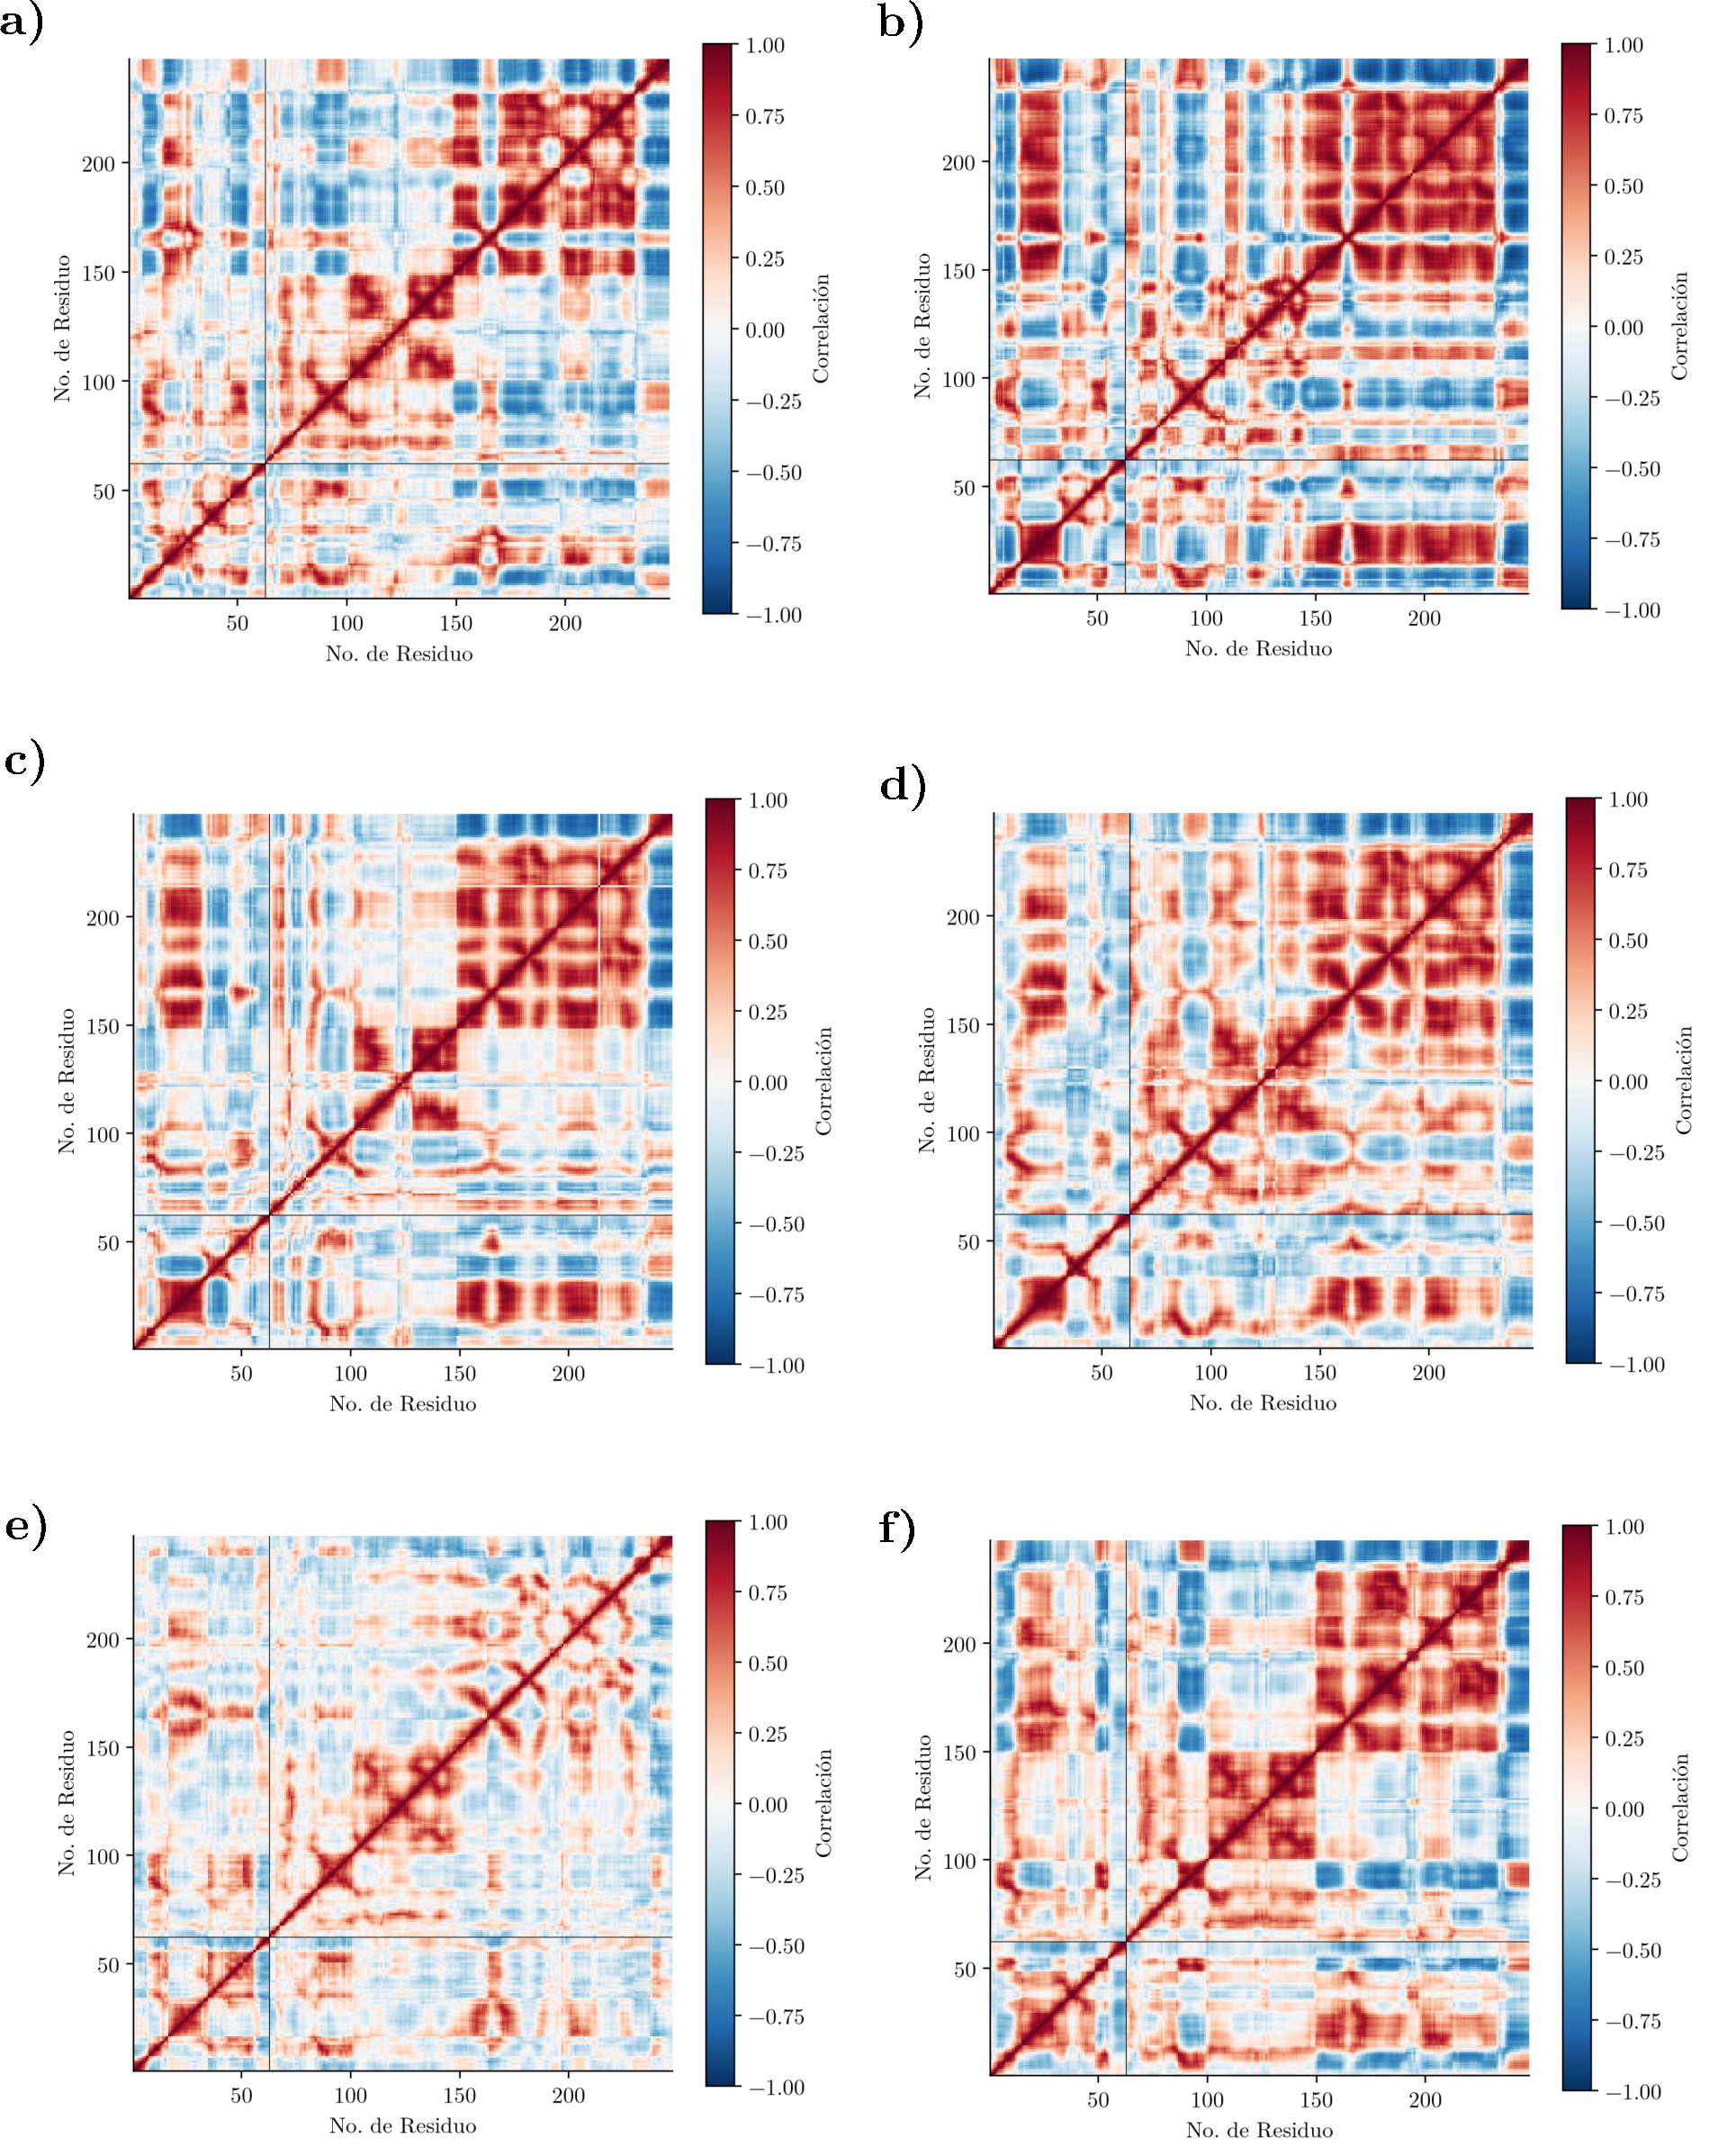
\includegraphics[width=0.90\textwidth]{imagenes/Resu/dccm.pdf}
    \caption{Evolución temporal del número de enlaces de hidrógeno intramoleculares formados en la proteína a lo largo de 100 ns.\textbf{a)} Sitio alostérico con el ligando C$_{60}$(Gly)$_{4}$; 
\textbf{b)} sitio alostérico con el ligando benzamida; 
\textbf{c)} sitio ortostérico con el ligando C$_{60}$(Gly)$_{4}$; 
\textbf{d)} sitio ortostérico con el ligando 246DA; 
\textbf{e)} acoplamiento ciego
\textbf{f)} proteína en su conformación nativa (estado inactivo abierto).}
    \label{fig:DDCM}
\end{figure}   

\newpage


\subsection*{Análisis de correlación cruzada dinámica:  alostérico C\textsubscript{60}(Gly)\textsubscript{4} vs. NS2B-NS3}

Al comparar la matriz de correlación cruzada dinámica (DCCM) de la alostérico C\textsubscript{60}(Gly)\textsubscript{4} frente al \textbf{NS2B-NS3}, se observa una elevada conservación de la topología dinámica global de la proteína. Ambas matrices exhiben tres dominios principales de movimiento coordinado (correlación positiva, a lo largo de la diagonal principal:

\begin{itemize}
    \item \textbf{Región 1 a 50:} Presenta un bloque de correlación positiva bien definido. En Alostérico C\textsubscript{60}(Gly)\textsubscript{4}, esta región mantiene la misma coherencia de movimiento que en el estado Apo, mostrando una marcada anticorrelación con el bloque C-terminal (residuos $150$--$220$). Este patrón contrapuesto refleja un movimiento colectivo de tipo ``bisagra'' o apertura/cierre entre ambos dominios.
    
    \item \textbf{Región 50 a 100:} En el estado Apo de NS2B-NS3 se aprecia una fuerte correlación intra-dominio ($0.50$ a $1.00$). En Alostérico C\textsubscript{60}(Gly)\textsubscript{4}, este bloque rojo se mantiene, aunque con una ligera redistribución de la intensidad de las correlaciones secundarias. Esta sutil variación sugiere una modulación local de la flexibilidad inducida por la presencia del ligando en la cavidad.
    
    \item \textbf{Región 150 a 240:} Constituye el dominio correlacionado más extenso y rígido de la estructura. En alostérico C\textsubscript{60}(Gly)\textsubscript{4} se conserva la integridad de este bloque concertado, observándose únicamente ligeras reducciones en las bandas de anticorrelación periféricas con respecto al segmento $50$--$100$ en comparación con el estado Apo.
\end{itemize}

\textbf{Interpretación:} La preservación del patrón de correlación en Alostérico C\textsubscript{60}(Gly)\textsubscript{4}indica que la unión del ligando en este modo de acoplamiento no altera ni desestabiliza los movimientos esenciales ni la comunicación alostérica nativa del receptor. Las pequeñas fluctuaciones observadas corresponden a la acomodación conformacional local del bolsillo catalítico/de unión ante el ligando, manteniendo la estabilidad macroestructural observada en el estado libre.

\subsection*{Análisis de correlación cruzada dinámica: acoplamiento ciego vs estado de la proteína NS2B-NS3}

A diferencia de lo observado en la Pose 61, la comparación de la \textbf{Pose 72} frente al \textbf{estado Apo pareado} revela una alteración drástica en el patrón global de correlación. La matriz de la Pose 72 exhibe una pérdida generalizada de intensidad en los bloques correlacionados y anticorrelacionados, pasando a estar dominada por regiones neutras de color blanco y tonos claros, lo cual evidencia un desacoplamiento dinámico significativo:

\begin{itemize}
    \item \textbf{Región 1 a 50:} Muestra una marcada atenuación del bloque de correlación positiva en comparación con el estado Apo, reduciéndose a valores débiles ($0.00$ a $0.50$). Asimismo, las bandas de anticorrelación hacia el extremo C-terminal pierden su definición nativa.
    
    \item \textbf{Región 50 a 100:} En lugar del bloque fuertemente coordinado característico de la proteína libre, la Pose 72 presenta parches muy dispersos de baja correlación ($0.00$ a $0.50$) mezclados con amplias zonas neutras, lo que señala la interrupción de la movilidad coordinada en este segmento.
    
    \item \textbf{Región 100 a 150:} Se observan únicamente focos aislados de correlación ($0.00$ a $0.75$) restringidos a la diagonal. Prevalecen las zonas de anticorrelación neutra o débil ($0.00$ a $-0.25$), indicando que la fluctuación de estos aminoácidos se vuelve predominantemente independientes.
    
    \item \textbf{Región 150 a 240:} Aunque conserva cierta coherencia local muy cerca de la diagonal principal ($0.00$ a $0.50$), la Pose 72 carece de los bloques continuos intensos y de las bandas de anticorrelación globales característicos del estado Apo libre.
\end{itemize}

\textbf{Interpretación:} El modo de unión en el acoplamiento ciego (genera un impacto profundo en la dinámica interna del receptor. La sustitución de los bloques coordinados por regiones de correlación nula ($0.00$) demuestra que la presencia del ligando en esta postura desacopla los movimientos colectivos esenciales de la proteína. En consecuencia, los residuos adquieren una movilidad estocástica e independiente, interrumpiendo la comunicación alostérica nativa observada en el estado Apo.

\subsection*{Análisis de correlación cruzada dinámica: ortostérico con el ligando C$_{60}$(Gly)$_{4}$  vs. estado de la proteína NS2B-NS3}

Al analizar la matriz de correlación cruzada dinámica (DCCM) del ligando C$_{60}$(Gly)$_{4}$;  en comparación con el \textbf{estado Apo de la proteína NS2B-NS3}, se aprecia una notable conservación de la arquitectura dinámica nativa, caracterizada por la presencia de dominios fuertemente consolidados tanto en correlación positiva  como en anticorrelación:

\begin{itemize}
    \item \textbf{Región 1 a 50:} Muestra una sólida correlación positiva intra-dominio ($0.50$ a $1.00$), prácticamente idéntica al estado Apo. Destaca una intensa banda de anticorrelación en azul oscuro  con respecto al bloque C-terminal (residuos $150$--$220$), confirmando un movimiento coordinado opuesto (mecanismo de ``bisagra'') que se mantiene fuertemente acoplado en esta pose.
    
    \item \textbf{Región 50 a 100:} Exhibe un bloque compacto de correlación positiva muy definido ($0.50$ a $1.00$) a lo largo de la diagonal principal. A diferencia del desacoplamiento visto en la conformación del C$_{60}$(Gly)$_{4}$-ciego , en el ligando C$_{60}$(Gly)$_{4}$ la comunicación interna de este dominio se preserva íntegramente, conservando sus fronteras de correlación bien delimitadas.
    
    \item \textbf{Región 150 a 240:} Constituye el dominio más rígido y concertado de la proteína, alcanzando valores de correlación cercanos a $1.00$ (rojo intenso). Además, muestra zonas de anticorrelación cruzada muy nítidas con respecto a los dominios N-terminales, lo que evidencia una respuesta estructural rígida y altamente coordinada ante la dinámica del sistema.
\end{itemize}

\textbf{Interpretación:} El complejo ligando C$_{60}$(Gly)$_{4}$ demuestra conservar la red de comunicación y los modos de vibración esenciales característicos del estado libre (Apo). La nitidez y ligera acentuación de las bandas de anticorrelación sugieren que este modo de acoplamiento del ligando no solo respeta la dinámica global del receptor, sino que promueve una mayor estabilización de los movimientos concertados de cierre y apertura entre dominios.

\subsection*{Análisis de correlación cruzada dinámica: ortostérico con el ligando 246DA  vs. estado de la proteína NS2B-NS3}

Al analizar la matriz de correlación cruzada dinámica (DCCM) del ligando 246DA en comparación con el \textbf{estado Apo pareado}, se observa un patrón altamente estructurado con una distribución de correlaciones muy similar a la del estado libre, conservando los modos de movimiento esenciales de la proteína. Sin embargo, la Pose 03 se distingue por presentar un mayor contraste y nitidez en las bandas de correlación y anticorrelación con respecto al estado Apo libre:

\begin{itemize}
    \item \textbf{Región 1 a 50:} Muestra una sólida correlación positiva intra-dominio. En comparación con el estado Apo, esta Pose exhibe una definición más nítida y acentuada en las regiones de anticorrelación  hacia los residuos C-terminales, confirmando una clara sincronización en dirección opuesta (mecanismo de tipo ``bisagra'').
    
    \item \textbf{Región 50 a 100:} Presenta un bloque compacto de correlación positiva bien delimitado a lo largo de la diagonal principal. Este segmento se encuentra delimitado por franjas de anticorrelación ($0.00$ a $-0.50$), lo que evidencia que la interacción con el ligando en la Pose 03 confiere una mayor definición estructural y confinamiento dinámico a este dominio con respecto a la proteína libre.
    
    \item \textbf{Región 150 a 240:} Constituye el dominio más rígido y fuertemente coordinado de la estructura, alcanzando intensidades de correlación positiva muy elevadas (rojo oscuro). La Pose 03 resalta por consolidar este bloque C-terminal con mayor fuerza que el estado Apo, mostrando además bandas de anticorrelación extremadamente marcadas en relación con los dominios N-terminales.
\end{itemize}

\textbf{Interpretación:} El ligando 246DA induce una estabilización acentuada en la proteína, promoviendo una respuesta dinámica caracterizada por una mayor rigidez en el dominio C-terminal y un acoplamiento más fuerte en los movimientos colectivos de apertura y cierre. Aunque se aprecian ligeras zonas de difuminación neutra  en la periferia de la diagonal principal correspondientes a fluctuaciones locales independientes, la firma dinámica global demuestra que el ligando 246DA optimiza y consolida la red de comunicación alostérica nativa de la macromolécula.

\subsection*{Análisis de correlación cruzada dinámica: alostérico con el ligando de benzamida;  vs. estado de la proteína NS2B-NS3}

El ligando benzamida destaca por presentar el mayor grado de acoplamiento y sincronización colectiva entre todas las posturas evaluadas. En comparación con el estado de la proteína apo-NS2B-NS3, la matriz del ligando benzamida exhibe un drástico incremento en la intensidad y extensión tanto de las correlaciones positivas  como de las anticorrelaciones , reduciendo significativamente las regiones neutras o independientes:

\begin{itemize}
    \item \textbf{Región 1 a 50:} Muestra un bloque intra-dominio fuertemente correlacionado en rojo intenso ($0.50$ a $1.00$). Presenta bandas de anticorrelación cruzada extremadamente marcadas en azul oscuro  con respecto a la región C-terminal ($150$--$240$), lo que evidencia un movimiento concertado opuesto sumamente acoplado y definido.
    
    \item \textbf{Región 50 a 100:} Exhibe un bloque de correlación positiva muy compacto y saturado a lo largo de la diagonal principal ($0.50$ a $1.00$). A diferencia del estado apo-NS2B-NS3, las franjas de anticorrelación que delimitan este segmento se vuelven más gruesas y continuas, reflejando una interacción rígida y coordinada con el resto del entramado proteico.
    
    \item \textbf{Región 150 a 240:} Constituye el bloque rígido más extenso y consolidado de la estructura, alcanzando valores de correlación cercanos a $1.00$ de manera prácticamente uniforme. Este dominio actúa como un bloque macroestructural altamente cohesivo que se desplaza en dirección opuesta a los dominios N-terminales con la máxima coherencia del sistema.
\end{itemize}

\textbf{Interpretación:} Maximiza la red de comunicación alostérica y la correlación de movimientos a larga distancia dentro del receptor. Este modo de acoplamiento del ligando promueve un hiper-acoplamiento dinámico que rigidiza los dominios principales y acentúa con gran claridad los modos colectivos nativos de apertura y cierre (mecanismo de bisagra), funcionando como un potente estabilizador de la dinámica global de la proteína.

\subsection*{Inhibición del $C_{60}\text{-(Gly)}_4$}

El análisis comparativo de las matrices de correlación cruzada dinámica (DCCM) entre los controles de referencia y los modos de acoplamiento del derivado $C_{60}\text{-(Gly)}_4$ permite deducir el comportamiento mecanístico de la macromolécula frente a la inhibición ortostérica y alostérica:

\begin{enumerate}
    \item \textbf{Inhibición alostérica (compuesto benzamida):} La interacción del $C_{60}\text{-(Gly)}_4$ en la cavidad alostérica reportada para la benzamida (Pose 61) exhibe una topología dinámica análoga a la del inhibidor alostérico de referencia (Pose 01) y a la del estado Apo pareado. La preservación de los bloques de correlación y de las bandas de anticorrelación inter-dominio confirma que el ligando se acomoda eficazmente en el sitio alostérico sin perturbar los modos colectivos nativos ni la estabilidad global del receptor.

    \item \textbf{Inhibición ortostérica (compuesto 246DA):} El acoplamiento en el sitio activo ortostérico induce una acentuación en la nitidez de las correlaciones y anticorrelaciones cruzadas, comportamiento que mimetiza la respuesta generada por el inhibidor ortostérico de referencia en la estructura de la proteína. Este perfil evidencia un empaquetamiento rígido del dominio C-terminal y la consolidación del mecanismo de apertura/cierre (bisagra), respaldando la capacidad del $C_{60}\text{-(Gly)}_4$ para actuar como un inhibidor ortostérico altamente efectivo.

    \item \textbf{Especificidad del acoplamiento ciego:}
 La pérdida generalizada de coherencia dinámica caracterizada por la atenuación de las bandas de correlación y la prevalencia de regiones neutras demuestra que la unión inespecífica del $C_{60}\text{-(Gly)}_4$ desacopla la comunicación alostérica nativa. Este contraste resalta la relevancia topológica de los sitios ortostérico y alostérico específicos, los cuales son indispensables para inducir una respuesta conformacional funcionalmente relevante.
\end{enumerate}

\textbf{Conclusión General:} El derivado $C_{60}\text{-(Gly)}_4$ demuestra una notable dualidad inhibitoria, siendo capaz de estabilizar la dinámica macroestructural de la proteína tanto en la cavidad ortostérica como en la alostérica mediante firmas de correlación equiparables a los fármacos/controles de referencia (246DA y benzamida, respectivamente).

\begin{figure}[H]
    \centering
    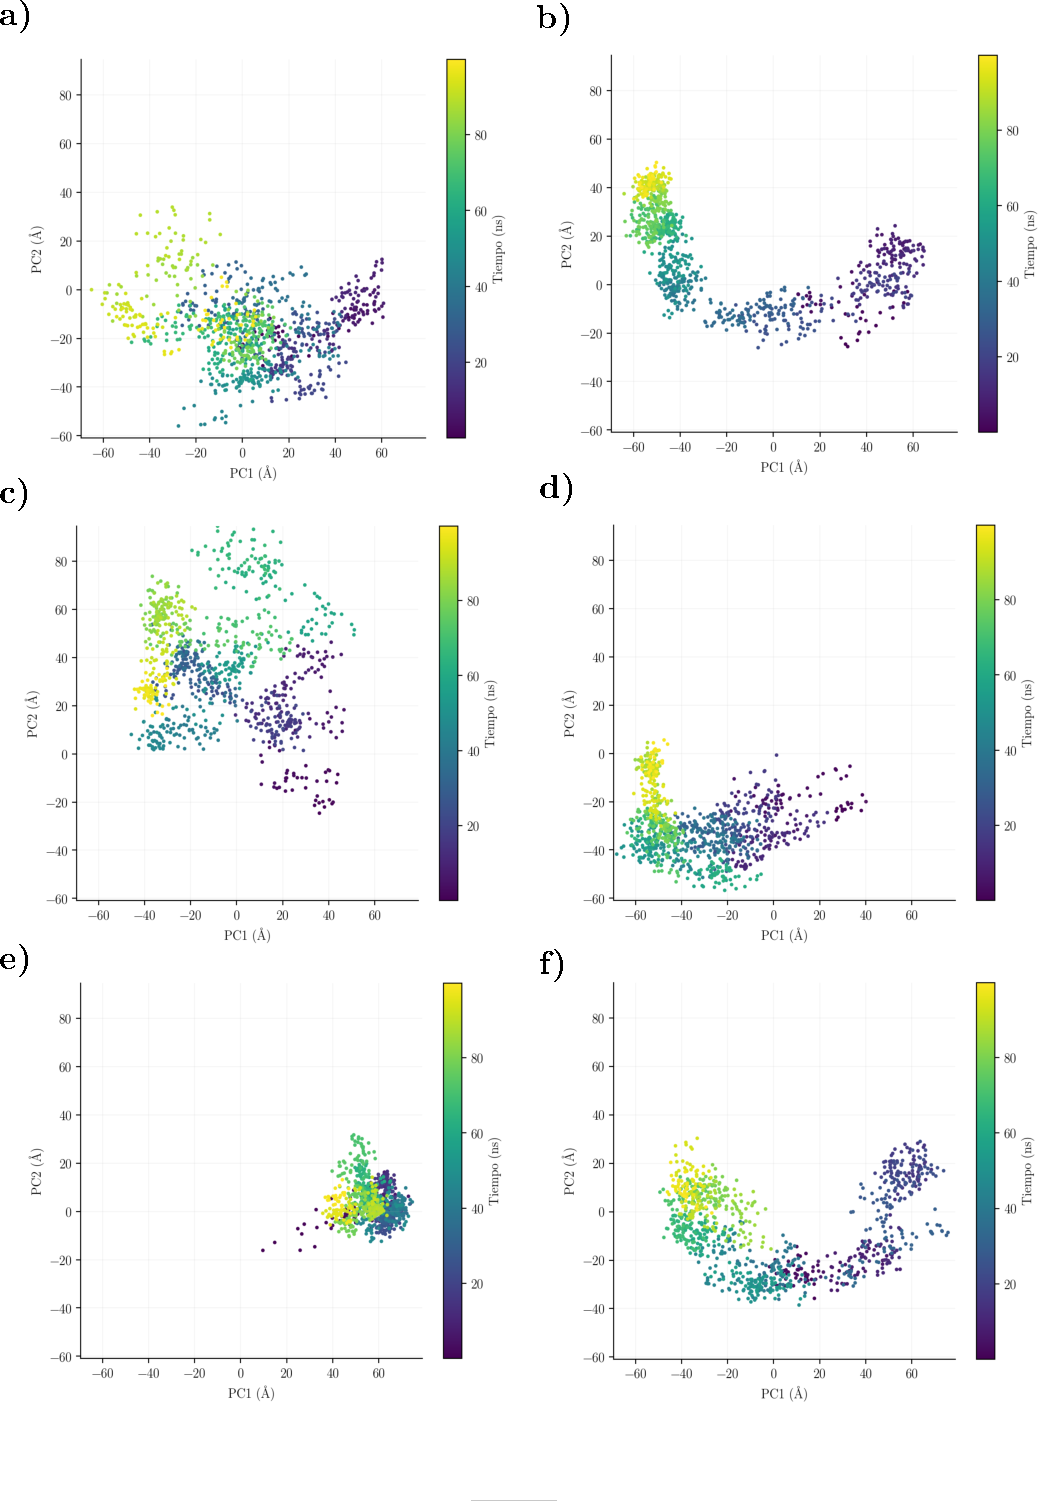
\includegraphics[width=0.80\textwidth]{imagenes/Resu/pca-common.pdf}
   \caption{\textbf{Evolución temporal del espacio conformacional (PCA común).} 
\textbf{a)} sitio alostérico con el ligando C$_{60}$(Gly)$_{4}$; 
\textbf{b)} sitio alostérico con un derivado de benzamida; 
\textbf{c)} sitio ortostérico con el ligando C$_{60}$(Gly)$_{4}$; 
\textbf{d)} sitio ortostérico con el ligando 246DA; 
\textbf{e)} acoplamiento ciego
\textbf{f)} proteína en su conformación nativa (estado inactivo abierto).}
    \label{fig:PCA-common}
\end{figure}   

En la Figura~\ref{fig:PCA-common} se presenta el análisis de componentes principales compartidos (PCA Common) proyectado a lo largo de 100~ns de simulación para los seis sistemas evaluados (paneles a--f). El eje $X$ representa el primer componente principal ($PC1$), el cual describe el modo colectivo de movimiento de mayor amplitud estructural (como transiciones globales de apertura o cierre). Por su parte, el eje $Y$ corresponde al segundo componente principal ($PC2$), que captura el segundo modo de movimiento colectivo ortogonal e independiente a $PC1$. La escala cromática representa la evolución temporal de la trayectoria, transitando desde el tiempo inicial (0~ns, morado/azul) hasta el tiempo final (100~ns, amarillo).

El sistema alostérico $\text{C}_{60}(\text{Gly})_4$ (\textbf{a}) muestra una amplia dispersión conformacional, iniciando en valores positivos de $PC1$ ($\approx 60\text{ \AA}$) y desplazándose hacia regiones de $PC2 \approx 30\text{ \AA}$ en los tiempos finales de simulación. Aunque el sistema muestra cierta estabilidad al final de la trayectoria, la presencia del compuesto promueve un comportamiento dinámico y fluctuante. En contraste, el sistema alostérico benzamida (\textbf{b}) exhibe una transición conformacional altamente direccionada en forma de arco, la cual inicia en $PC1 \approx 50\text{ \AA}$ y evoluciona de manera continua hasta alcanzar valores de $PC2 \approx 40\text{ \AA}$. Esta trayectoria sugiere que, si bien la estructura mantiene un comportamiento dinámico, transita hacia un estado final bien definido y estable.

Por otro lado, el sistema otostérico $\text{C}_{60}(\text{Gly})_4$ (\textbf{c}) presenta una variación conformacional sustancial en ambos componentes, alcanzando valores de $PC2$ inusualmente elevados ($\approx 40\text{ a }80\text{ \AA}$) entre los 50 y 100~ns. Esto indica que el ligando acoplado al sitio otostérico induce perturbaciones estructurales severas y modos de movimiento no explorados por los demás sistemas. En contraste, el ligando ortostérico 246DA (\textbf{d}) evoluciona progresivamente desde $PC1$ positivo hacia regiones de $PC1$ negativo y $PC2$ entre $-20$ y $-40\text{ \AA}$, evidenciando una dinámica estructural coordinada y con menor amplitud de fluctuación.

El sistema de restricción (\textbf{e}, Ciego) se mantiene confinado en una región sumamente acotada del espacio vectorial ($PC1 \approx 0\text{ \AA}$, $PC2 \approx 0\text{ \AA}$) durante los 100~ns, lo que confirma una drástica pérdida de flexibilidad y la incapacidad de explorar el espacio conformacional. Finalmente, la proteína libre (\textbf{f}, Apo 2FOM) despliega una transición amplia e intrínseca desde $PC1 \approx 50\text{ \AA}$ hasta $PC1 \approx -40\text{ \AA}$, representando el patrón de movilidad natural del sistema en ausencia de ligandos.

Al comparar la influencia de los compuestos frente al estado apoproteico (\textbf{f}), se observa que el sistema alostérico benzamida (\textbf{b}) y el ortostérico 246DA (\textbf{d}) son los que mejor conservan una dinámica ordenada y estable. Por el contrario, los derivados de $\text{C}_{60}(\text{Gly})_4$ (\textbf{a} y \textbf{c}) introducen fluctuaciones atípicas o dispersiones mayoritarias, demostrando que la naturaleza química y la ubicación del sitio de unión (alostérico vs. otostérico/ortostérico) modulan de forma diferenciada el paisaje dinámico de la macromolécula.


\begin{figure}[H]
    \centering
    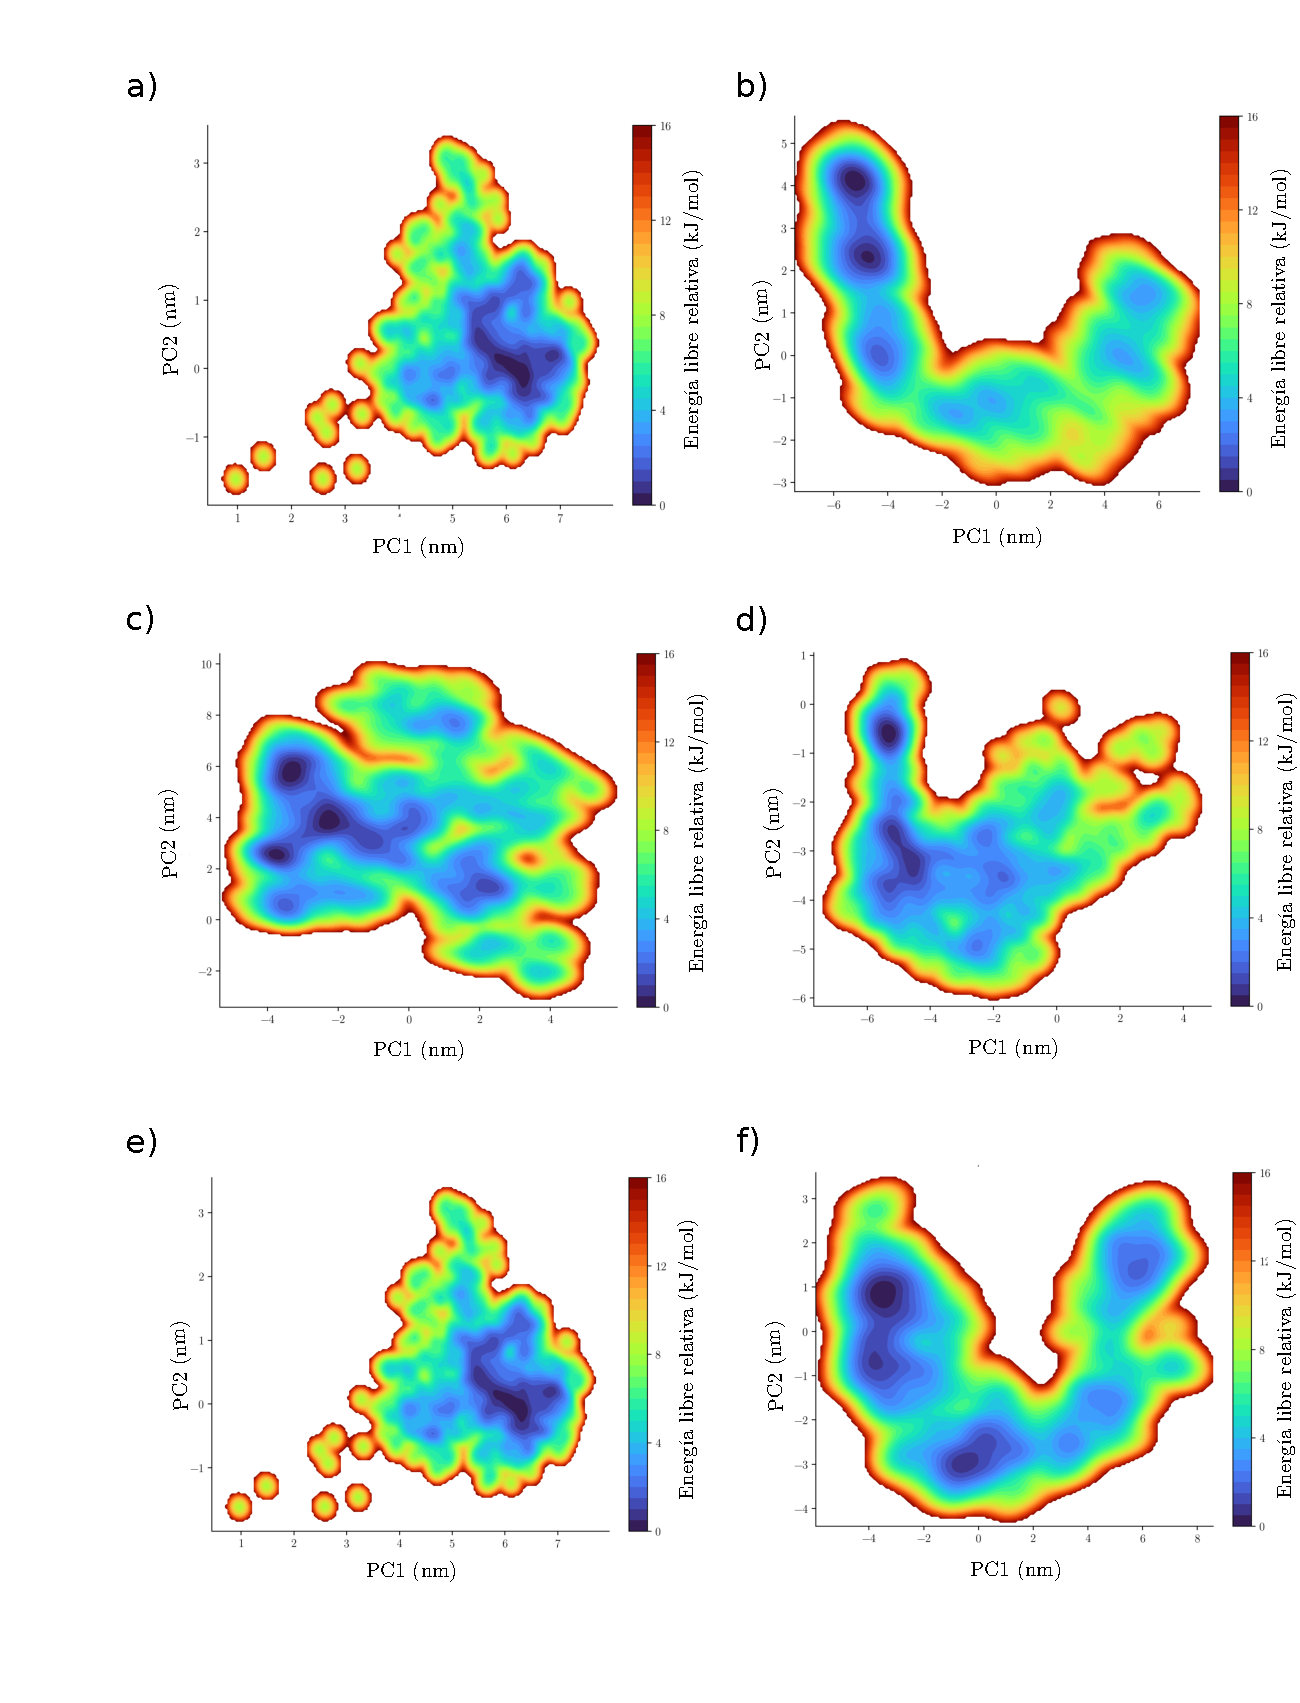
\includegraphics[width=0.90\textwidth]{imagenes/Resu/fel.pdf}
    \caption{\textbf{Paisaje de energía libre (FEL) en el espacio conformacional.} 
\textbf{a)} sitio alostérico con el ligando C$_{60}$(Gly)$_{4}$; 
\textbf{b)} sitio alostérico con el ligando de benzamida; 
\textbf{c)} sitio ortostérico con el ligando C$_{60}$(Gly)$_{4}$; 
\textbf{d)} sitio ortostérico con el ligando 246DA; 
\textbf{e)} acoplamiento ciego
\textbf{f)} proteína en su conformación nativa (estado inactivo abierto).}
   
    \label{fig:pca-fel}
\end{figure} 

En la Figura~\ref{fig:pca-fel} se muestra el paisaje de energía libre (FEL, por sus siglas en inglés) proyectado sobre el plano cartesiano PC1 vs. PC2 para los seis sistemas estudiados (paneles a--f). A diferencia de la representación temporal, el mapa de FEL evalúa la estabilidad termodinámica y la probabilidad poblacional de las conformaciones exploradas durante la simulación. La barra de color representa la energía libre relativa ($\Delta G$), medida en $\text{kJ/mol}$, calculada mediante la relación de Boltzmann. Las zonas azul oscuro corresponden a los valles o pozos de mínima energía ($\Delta G = 0.0\text{ kJ/mol}$), representando los estados conformacionales más estables y termodinámicamente favorecidos. Por su parte, las regiones cian, verdes y amarillas representan pendientes de mayor costo energético ($\Delta G \approx 4.0\text{ a }12.0\text{ kJ/mol}$), delimitadas por un límite superior de $16.0\text{ kJ/mol}$.

El estado apoproteico de referencia (\textbf{f}, NS2B-NS3) presenta un paisaje energético multimodal de amplia extensión, caracterizado por dos pozos principales de mínima energía: uno ubicado en el cuadrante superior izquierdo ($\text{PC1} \approx -4.0\text{ nm}$, $\text{PC2} \approx 0.8\text{ nm}$) y otro en la región inferior ($\text{PC1} \approx -1.0\text{ nm}$, $\text{PC2} \approx -2.8\text{ nm}$), acompañados por una cuenca secundaria accesible en el extremo derecho ($\text{PC1} \approx 5.5\text{ nm}$, $\text{PC2} \approx 1.5\text{ nm}$). Este perfil refleja la plasticidad estructural intrínseca de la proteína libre en su estado abierto inactivo (2FOM), la cual transita entre múltiples mínimos de energía separados por barreras energéticas moderadas.

En contraposición, el sistema de control (\textbf{e}, Ciego) exhibe un pozo de energía altamente concentrado y delimitado alrededor de $\text{PC1} \approx 6.0\text{ nm}$ y $\text{PC2} \approx 0.0\text{ nm}$, junto con pequeñas poblaciones discretas transitorias a valores menores de PC1 ($\text{PC1} \approx 1.0\text{--}3.5\text{ nm}$). Esto confirma que la restricción conformacional responde a un atrapamiento termodinámico en un pozo de elevada estabilidad local.

La incorporación de los distintos compuestos modula substancialmente la topografía del paisaje energético:

\begin{itemize}
    \item \textbf{Alostérico $\text{C}_{60}(\text{Gly})_4$ (a):} Muestra un pozo de mínima energía bien focalizado en $\text{PC1} \approx 6.0\text{ nm}$ y $\text{PC2} \approx 0.0\text{ nm}$, acompañado de pequeños microestados poblados de forma discontinua en la región de menor PC1 ($\text{PC1} \approx 1.0\text{--}3.5\text{ nm}$, $\text{PC2} \approx -1.5\text{ nm}$). Esta topografía indica un estado de equilibrio fuertemente desplazado hacia un único mínimo dominante.
    
    \item \textbf{Alostérico benzamida (b):} Es el sistema que despliega una reorganización del paisaje en forma de canal continuo en, conectando dos cuencas energéticas principales: un valle vertical alargado en la región izquierda ($\text{PC1} \approx -5.0\text{ nm}$) con múltiples mínimos locales ($\text{PC2} \approx 0.5\text{ nm}$, $2.5\text{ nm}$ y $4.0\text{ nm}$), y una cuenca secundaria en el extremo derecho ($\text{PC1} \approx 5.0\text{ nm}$, $\text{PC2} \approx 1.5\text{ nm}$). La existencia de este canal accesible demuestra que el ligando induce y estabiliza el equilibrio entre conformaciones funcionales discretas.
    
    \item \textbf{Ortostérico $\text{C}_{60}(\text{Gly})_4$ (c):} Provoca un desplazamiento drástico del pozo de mínima energía hacia coordenadas de PC2 elevadas ($\text{PC1} \approx -2.5\text{ a }-4.0\text{ nm}$, $\text{PC2} \approx 3.5\text{ a }6.0\text{ nm}$), con expansiones que alcanzan hasta $\text{PC2} \approx 10.0\text{ nm}$. La dispersión del pozo sugiere que la voluminosa estructura del fullereno en el sitio activo desestabiliza la conformación nativa y fuerza al complejo a explorar un espacio conformacional de mayor entropía.
    
    \item \textbf{Ortostérico 246DA (d):} Presenta una concentración dominante de la densidad poblacional en la región de PC1 negativo ($\text{PC1} \approx -5.5\text{ a }-3.5\text{ nm}$, $\text{PC2} \approx -0.5\text{ a }-3.5\text{ nm}$). Este pozo profundo y delimitado evidencia que el compuesto ortostérico estabiliza prioritariamente una conformación específica compacta, restringiendo la exploración conformacional hacia valores positivos de PC1.
\end{itemize}




\begin{figure}[H]
    \centering
    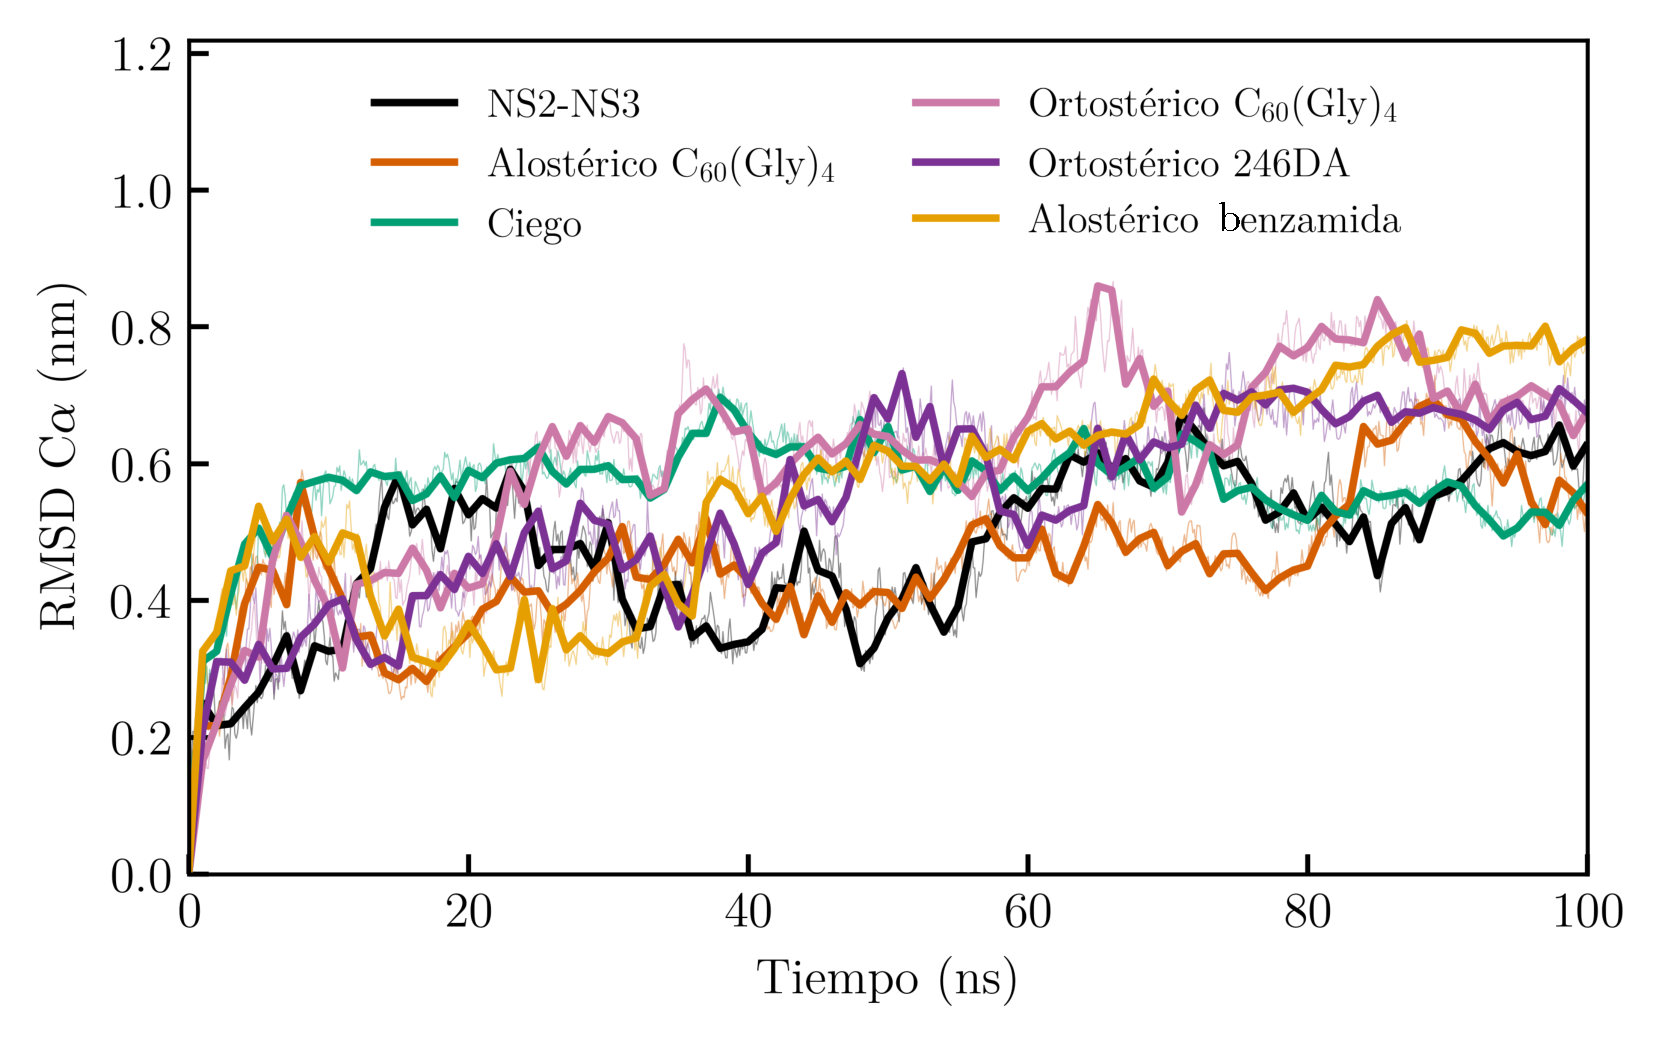
\includegraphics[width=0.7\textwidth]{imagenes/Resu/rmsd_ca.pdf}
    \caption{Evolución temporal de la desviación cuadrática media (RMSD) de los átomos C$\alpha$ del complejo enzimático NS2B-NS3 en estado libre (\textit{Apo}) y acoplado a los distintos inhibidores durante 100 ns de simulación.}
    \label{fig:RMSD}
\end{figure}   
Se evaluó la estabilidad estructural global del complejo enzimático NS2B-NS3 y sus respectivos complejos proteína-ligando mediante el cálculo de la desviación cuadrática media (RMSD) de los átomos C$\alpha$ a lo largo de 100 ns de simulación. (Figura~\ref{fig:RMSD}).

Durante los primeros 10 ns, todos los sistemas mostraron una fase inicial de relajación estructural en medio acuoso. A partir de los 15 ns, se observó una divergencia marcada en los perfiles de RMSD, lo que refleja respuestas conformacionales específicas dependientes del sitio de unión y del tipo de ligando acoplado. En general, los valores relativamente elevados de RMSD observados en todos los sistemas ($\ge 0.55\text{ nm}$) se justifican por el estado abierto e inactivo inicial del molde 2FOM, en el cual la región C-terminal del cofactor NS2B posee una alta flexibilidad intrínseca al no estar empaquetada sobre el centro activo.

La forma libre (\textit{Apo}-NS2B-NS3) mantuvo valores fluctuantes moderados ($0.35\text{--}0.45\text{ nm}$) hasta los 50 ns, momento en el cual experimentó un incremento progresivo hasta estabilizarse cerca de los $0.60\text{ nm}$. Este comportamiento refleja la transición conformacional y exploración del espacio de fases de la región flexible de NS2B, la cual busca estados estables en ausencia de un ligando que promueva el cierre del sitio activo.

En cuanto a los complejos evaluados:
\begin{itemize}
    \item El sistema \textbf{Ortostérico $C_{60}(\text{Gly})_4$} presentó los valores de RMSD más elevados ($\sim 0.75\text{--}0.85\text{ nm}$), lo que sugiere una reorganización severa del bolsillo catalítico y de las regiones adyacentes para dar cabida a la voluminosa estructura del ligando.
    \item Los complejos \textbf{alostérico benzamida} y \textbf{ortostérico 246DA} exhibieron fluctuaciones intermedias-altas, alcanzando un régimen estable entre $0.60$ y $0.75\text{ nm}$.
    \item El complejo acoplado en el sitio \textbf{Ciego} mostró un rápido ajuste inicial en los primeros 15 ns, manteniendo posteriormente una meseta notablemente estable alrededor de los $0.55\text{--}0.60\text{ nm}$.
    \item El complejo \textbf{Alostérico $C_{60}(\text{Gly})_4$} mostró un comportamiento singular con una contracción conformacional entre los 20 y 50 ns (descendiendo hasta $\sim 0.35\text{ nm}$), consistente con un proceso de empaquetamiento y ajuste inducido hacia un estado más compacto antes de alcanzar su equilibrio final ($\sim 0.60\text{ nm}$).
\end{itemize}

A pesar de las diferencias en la magnitud de la desviación, todos los perfiles alcanzaron un estado de meseta fluctuante a partir de los 60 ns hasta el final de la simulación, confirmando la convergencia estructural de los sistemas hacia nuevos mínimos de energía metaestables partiendo de la conformación abierta de la proteina NS2B-NS3.

\begin{figure}[H]
    \centering
    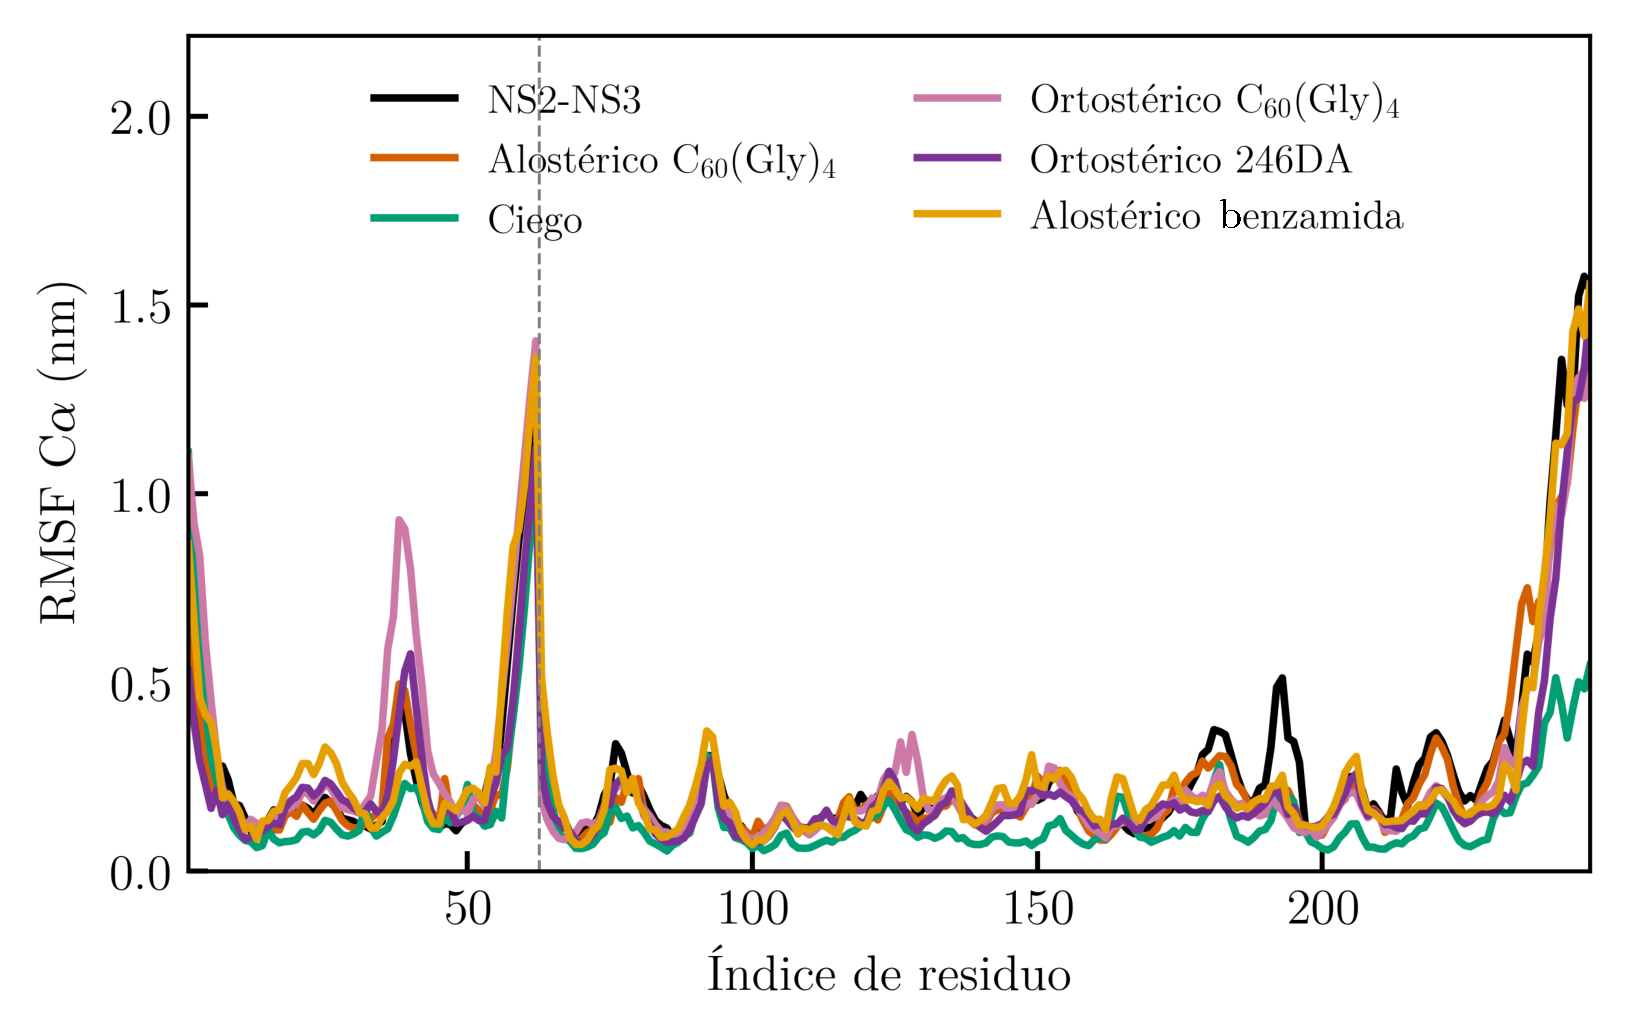
\includegraphics[width=0.7\textwidth]{imagenes/Resu/rmsf_ca.pdf}
    \caption{Perfil de fluctuación cuadrática media (RMSF) por residuo para los átomos C$\alpha$ del complejo enzimático NS2B-NS3 en estado libre (\textit{Apo}) y acoplado a los distintos inhibidores durante 100 ns de simulación.}
    \label{fig:RMSF}
\end{figure}   

Para comprender las variaciones estructurales observadas en el RMSD, se analizó la movilidad local por residuo mediante el cálculo de la fluctuación cuadrática media (RMSF) de los átomos C$\alpha$ a lo largo de los 100 ns de simulación (Figura~\ref{fig:RMSF}). La línea vertical discontinua ($\sim$residuo 62) delimita el cofactor flexible NS2B (residuos 1--62) del dominio catalítico de la proteasa NS3 (residuos 63--250) del complejo heterodimérico NS2B-NS3.

En la cadena del cofactor NS2B, se observan dos zonas de alta movilidad. Alrededor del residuo 40, la unión del ligando \textbf{Ortostérico $C_{60}(\text{Gly})_4$} indujo un incremento notable en las fluctuaciones (1.0 nm), contrastando con la rigidez impuesta por el complejo \textbf{Ciego} (0.3 nm). Posteriormente, en la región $C$-terminal del cofactor (residuo 62), todos los sistemas mostraron un pico máximo de fluctuación (1.4-1.5 nm), lo que confirma la elevada movilidad intrínseca de esta zona.

En contraste, el dominio catalítico NS3 (residuos 63--220) mantuvo un núcleo estructural altamente estable, con valores de RMSF por debajo de 2 nm. No obstante, se identificó una diferencia funcional clave en la región de bucles comprendida entre los residuos 180 y 190: mientras que la proteína libre (\textit{Apo}-NS2B-NS3 línea negra) presentó un pico de movilidad de 0.5 nm, la formación de los complejos con ligando estabilizó este bucle, reduciendo el RMSF a valores 0.25 nm. Finalmente, el extremo $C$-terminal ($>$230 residuos) mostró la flexibilidad esperada en una región no estructurada, alcanzando 1.5 nm en la forma \textit{Apo} y en el complejo Alostérico, mientras que el sistema Ciego restringió significativamente esta movilidad a 0.55 nm.

Estos perfiles demuestran que el elevado RMSD global analizado previamente no obedece a una desnaturalización de la enzima, sino a la flexibilidad intrínseca del cofactor NS2B y de las extremidades terminales, mientras que la presencia de los ligandos ejerce un efecto estabilizador directo sobre los bucles del sitio activo en el dominio NS3.

\begin{figure}[H]
    \centering
    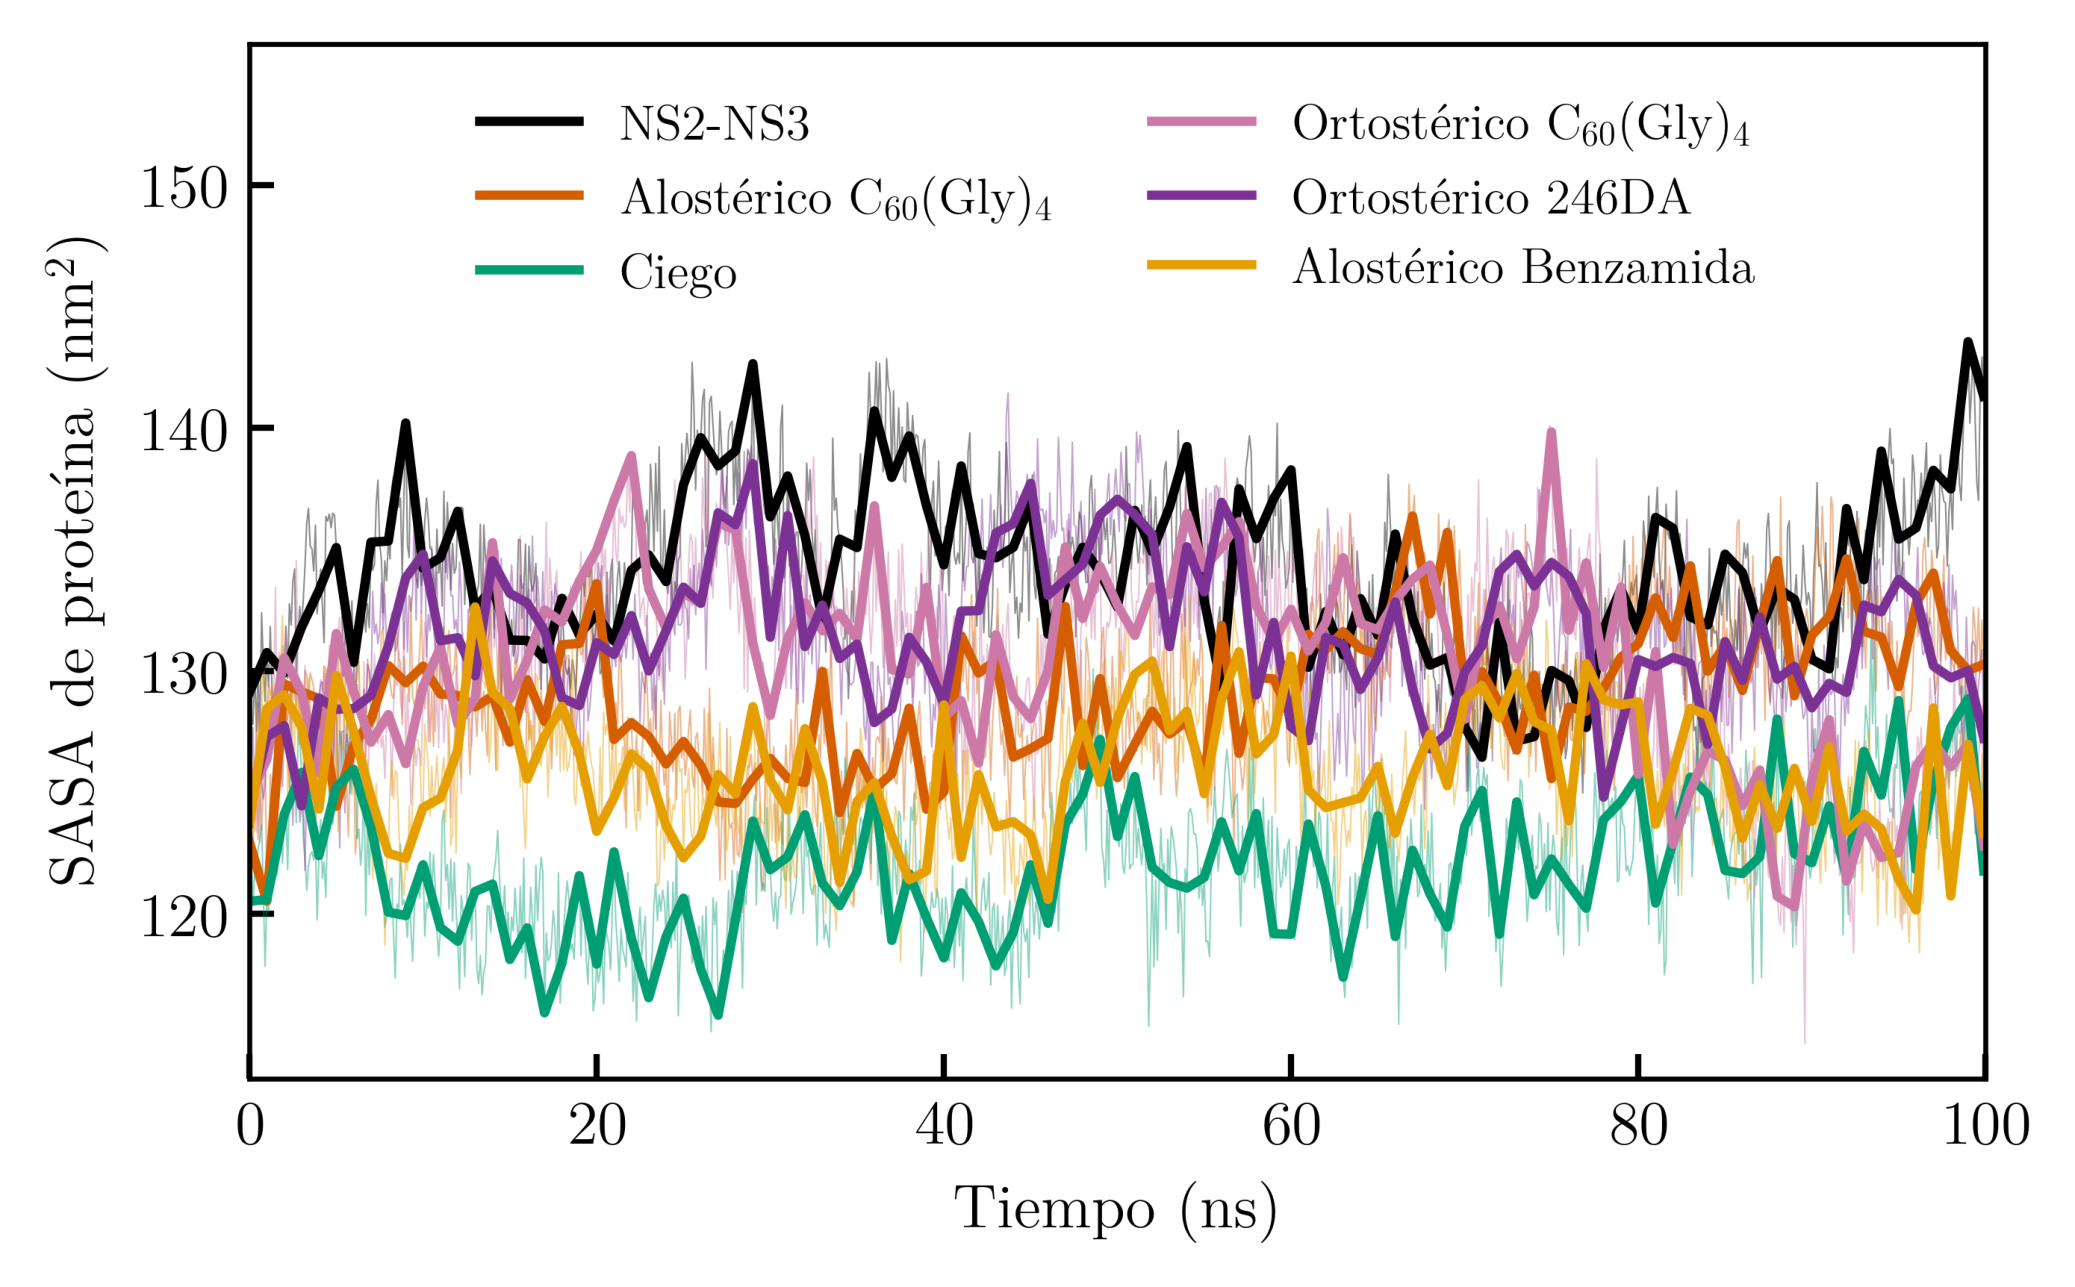
\includegraphics[width=0.6\textwidth]{imagenes/Resu/SASA.pdf}
    \caption{Evolución temporal del área de superficie accesible al solvente (SASA, en $\text{nm}^2$) para el complejo total (arriba), los ligandos (centro) y la proteína (abajo) a lo largo de 100 ns de simulación, tomando como referencia la proteasa NS2B-NS3.}
    \label{fig:sasa}
\end{figure}   
Para evaluar el grado de empaquetamiento estructural y el nivel de exposición al entorno acuoso, se calculó el área de superficie accesible al solvente (SASA, expresado en $\text{nm}^2$) durante los 100 ns de simulación para la proteína, los ligandos y los complejos totales (Figura~\ref{fig:sasa}).

El análisis del SASA de la proteína (panel inferior) muestra que la forma libre (\textbf{NS2-NS3}, línea negra) mantiene sostenidamente los valores más altos de exposición al solvente ($\sim 130\text{--}143\text{ nm}^2$) a lo largo de la trayectoria. Este comportamiento es coherente con el estado abierto e inactivo de la proteína NS2B-NS3, donde la elevada flexibilidad intrínseca del cofactor NS2B le permite fluctuar libremente en la interfaz acuosa sin empaquetarse de forma rígida sobre el dominio catalítico. 

Por el contrario, la acoplación de los distintos compuestos induce grados variables de aminoácidos hidrofobicos que se encuentran en contacto con el agua y compactación en la macromolécula:
\begin{itemize}
    \item El sistema de control \textbf{Ciego} (línea verde) exhibe la mayor reducción en el SASA proteico, fluctuando de forma notablemente estable entre $118$ y $126\text{ nm}^2$. Esta marcada disminución refleja un colapso o empaquetamiento conformacional que obstruye la superficie de la proteína respecto al agua.
    \item Los sistemas \textbf{Alostérico $\text{C}_{60}(\text{Gly})_4$} (naranja) y \textbf{Alostérico benzamida} (amarillo) muestran valores intermedios-bajos de SASA proteico ($\sim 122\text{--}132\text{ nm}^2$), confirmando que la modulación en el sitio alostérico favorece un estado ligeramente más compacto que el apoproteico.
    \item Los complejos ortostéricos \textbf{Ortostérico $\text{C}_{60}(\text{Gly})_4$} (rosa) y \textbf{Ortostérico 246DA} (morado) registran fluctuaciones iniciales altas ($\sim 130\text{--}140\text{ nm}^2$), seguidas de un descenso moderado hacia los 60 ns ($\sim 130\text{ nm}^2$), coincidiendo con la fase de estabilización previamente observada en el RMSD.
\end{itemize}

El comportamiento individual de los ligandos (panel central) revela diferencias críticas respecto a su acomodo en los bolsillos de unión:
\begin{itemize}
    \item El compuesto \textbf{Alostérico benzamida} (línea amarilla) presenta los valores de SASA más reducidos de todo el estudio ($\sim 0.5\text{--}1.5\text{ nm}^2$). Esto demuestra que la benzamida queda profundamente sepultada dentro de la cavidad alostérica, sufriendo un obstrucción casi completa frente al solvente.
    \item El ligando \textbf{Ortostérico 246DA} (línea morada) exhibe una alta exposición durante los primeros 55 ns ($\sim 5.0\text{--}5.5\text{ nm}^2$), la cual decae posteriormente a $\sim 4.0\text{ nm}^2$. Este cambio temporal evidencia un proceso de ajuste inducido donde el compuesto se reacomoda hacia el interior del sitio activo a partir de los 60 ns.
    \item Los derivados de fullereno \textbf{Alostérico $\text{C}_{60}(\text{Gly})_4$} y \textbf{Ortostérico $\text{C}_{60}(\text{Gly})_4$} mantienen una exposición moderada y constante ($\sim 3.5\text{--}4.5\text{ nm}^2$), lo que responde a la voluminosa esfera de carbono y las cadenas de glicina que permanecen parcialmente expuestas al solvente exterior.
\end{itemize}

Finalmente, el SASA total del complejo (panel superior) combina los efectos de empaquetamiento proteico y protuberancia del ligando, observándose que todos los sistemas convergen a perfiles estables a partir de los 60 ns. En conjunto, estos resultados corroboran que la unión de los inhibidores reduce la superficie expuesta de la proteasa NS2B-NS3, estabilizando estados conformacionales con un empaquetamiento superior al de la forma apoproteica.

 
\begin{figure}[H]
    \centering
    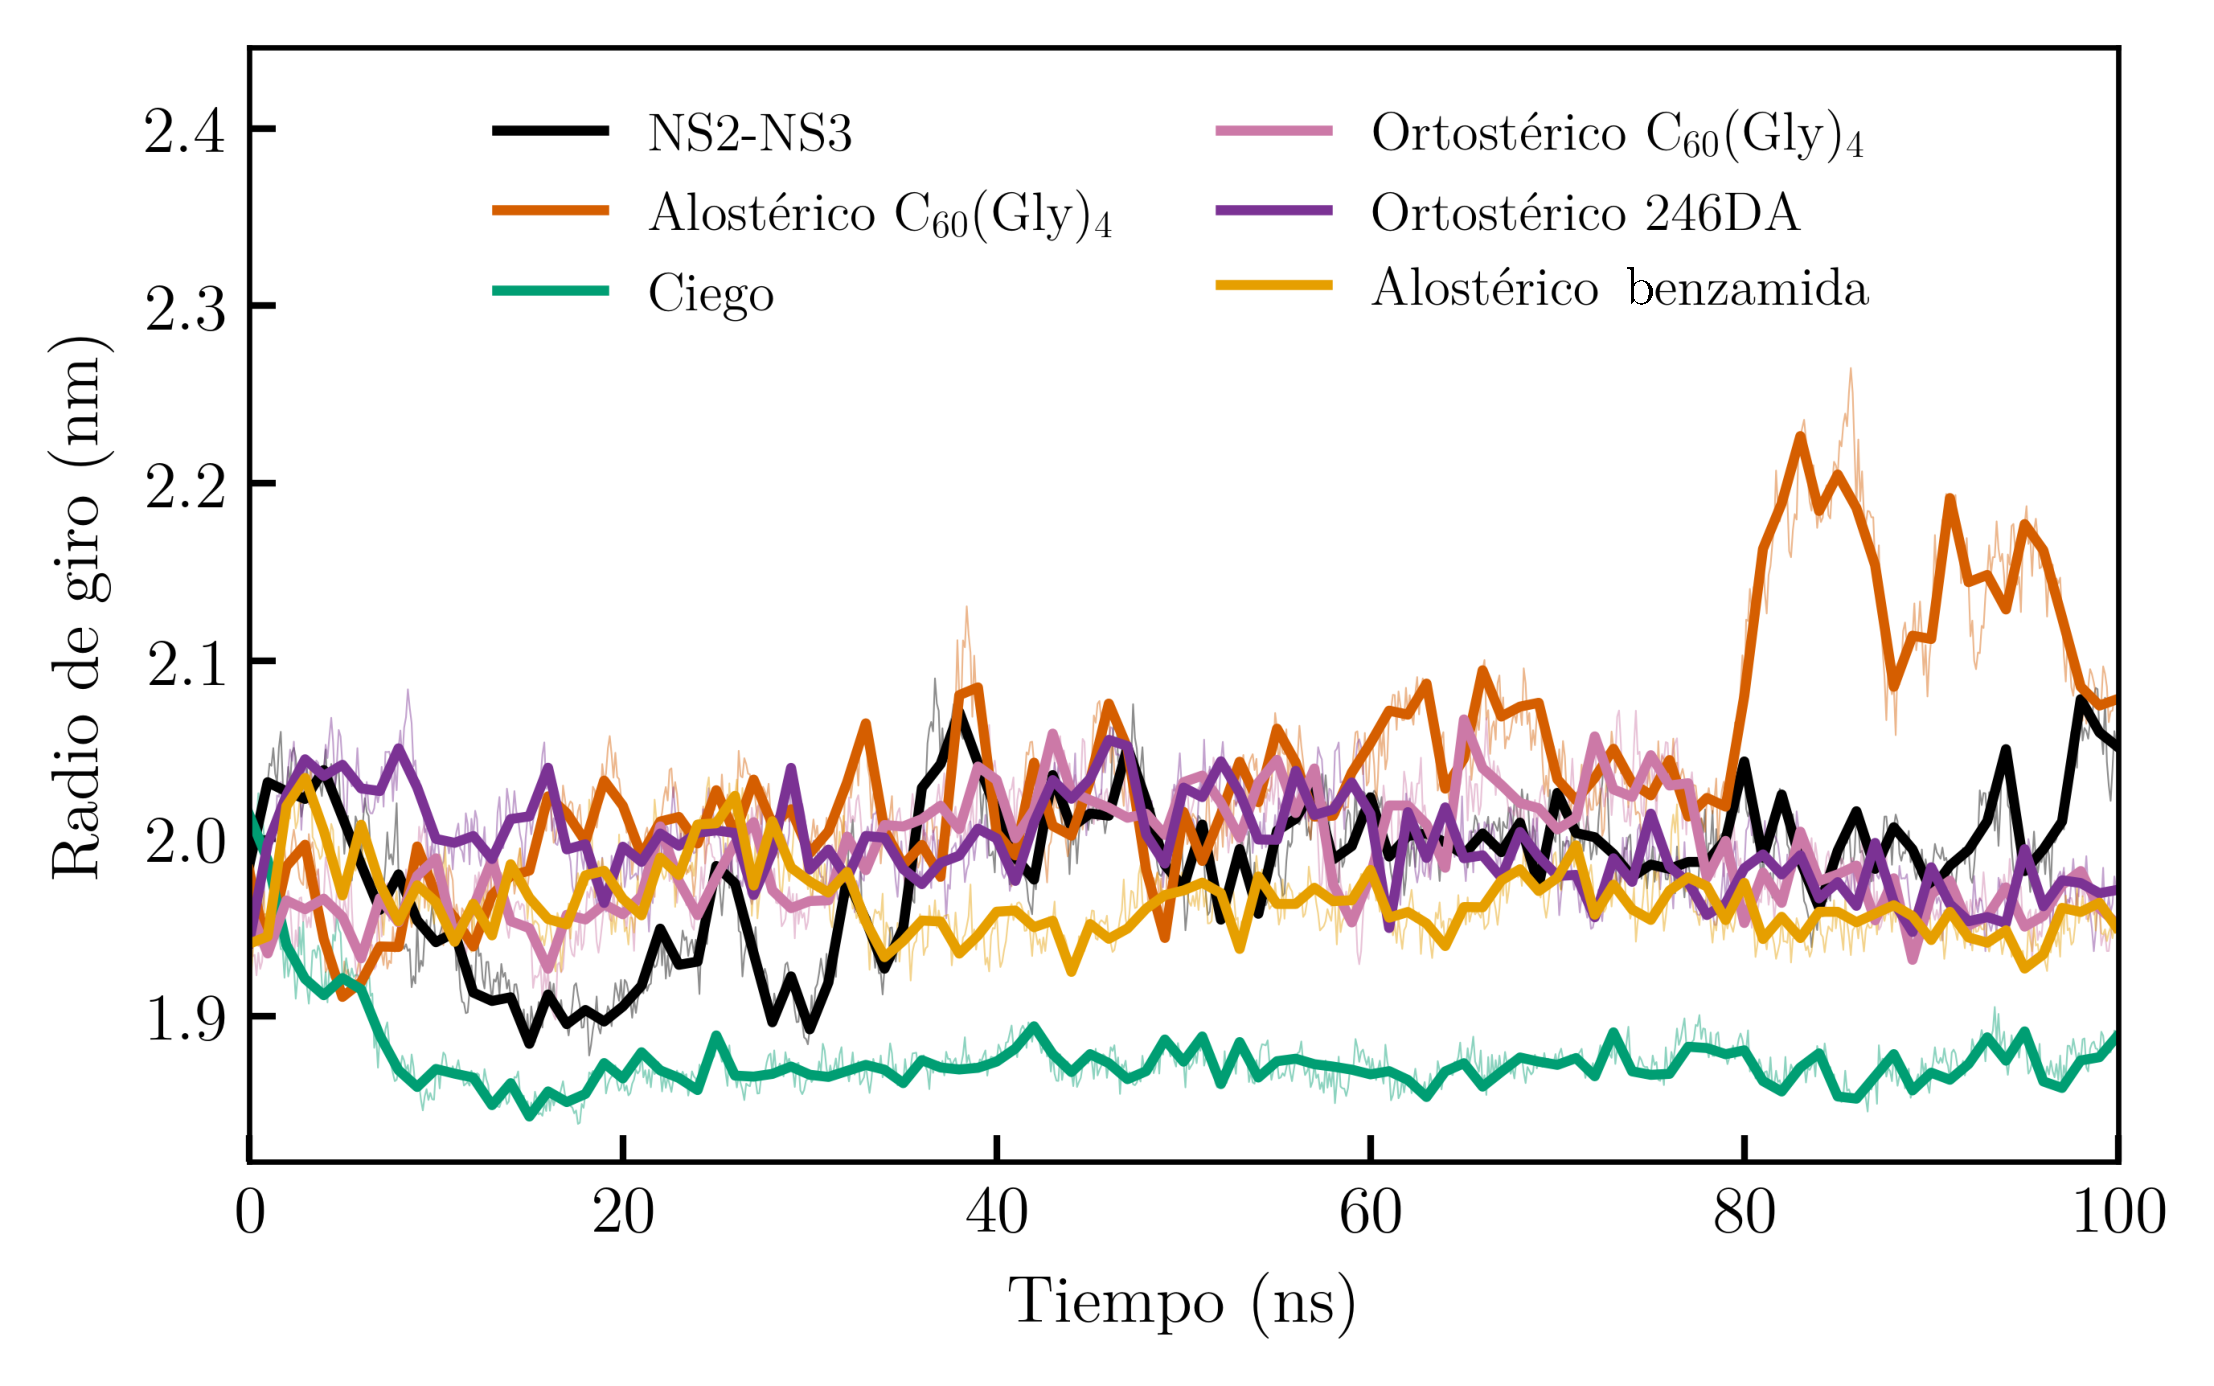
\includegraphics[width=0.7\textwidth]{imagenes/Resu/radio_giro.pdf}
    \caption{Evolución temporal del radio de giro en la proteína a lo largo de 100 ns.}
    \label{fig:RG}
\end{figure}   

En la Figura~\ref{fig:RG} se presenta la evolución temporal del radio de giro ($R_g$) a lo largo de 100 ns de simulación para la proteína libre (\textit{apo}, NS2B-NS3) y sus complejos con diversos ligandos.

Para la proteína libre (NS2B-NS3), el $R_g$ inicia en aproximadamente 2.0~nm y experimenta un descenso gradual durante los primeros 20--40~ns hasta alcanzar valores cercanos a 1.9~nm, lo cual refleja un incremento en la compacidad estructural y una menor extensión espacial. Posteriormente, el sistema se estabiliza de los 50 a los 80~ns, para finalmente presentar un incremento acentuado en el $R_g$ hacia los 90--100~ns (superando los 2.1~nm), lo que sugiere una transición hacia una conformación más abierta y flexible.

Al evaluar los complejos con inhibidores ortostéricos (\textit{Ortostérico $\text{C}_{60}\text{(Gly)}_4$} y \textit{Ortostérico 246DA}), se observa un perfil estructural bastante similar entre ambos. Tras pequeñas fluctuaciones durante los primeros 10~ns, ambos sistemas se estabilizan dentro de un rango de $R_g$ comprendido entre 1.9 y 2.0~nm, manteniendo la compacidad de la proteína libre sin inducir cambios conformacionales drásticos.

Por otro lado, los sistemas alostéricos exhiben comportamientos marcadamente contrapuestos:
\begin{itemize}
    \item El complejo \textbf{Alostérico benzamida} muestra la mayor estabilidad conformacional del conjunto, conservando un valor de $R_g$ sumamente constante (~2.0~nm) durante prácticamente toda la trayectoria.
    \item En contraste, el complejo \textbf{Alostérico $\text{C}_{60}$} presenta una clara alteración estructural hacia los 80~ns, donde el $R_g$ aumenta drásticamente hasta alcanzar valores cercanos a 2.25~nm. Este incremento marcado evidencia una pérdida de compacidad global y una mayor extensión espacial, consistente con un desdoblamiento parcial o una apertura conformacional de la proteína.
\end{itemize}

Finalmente, el sistema \textbf{Ciego} muestra un comportamiento peculiar y sumamente estable: mantiene los valores de $R_g$ más bajos de toda la simulación (alrededor de 1.85--1.90~nm) con fluctuaciones mínimas a lo largo de los 100~ns. Esta disminución sostenida respecto a la proteína libre indica que la interacción en este sitio promueve una mayor compacidad e induce un empaquetamiento estructural más denso.

\subsection{Conclusión}


